%	Begin the book
\begin{document}

% Copyright 2018-2023 Pietro Prandini
%
% This file is part of GuitarHub.
%
% GuitarHub is free software: you can redistribute it and/or modify
% it under the terms of the GNU General Public License as published by
% the Free Software Foundation, either version 3 of the License, or
% (at your option) any later version.
%
% GuitarHub is distributed in the hope that it will be useful,
% but WITHOUT ANY WARRANTY; without even the implied warranty of
% MERCHANTABILITY or FITNESS FOR A PARTICULAR PURPOSE.  See the
% GNU General Public License for more details.
%
% You should have received a copy of the GNU General Public License
% along with GuitarHub.  If not, see <https://www.gnu.org/licenses/>.

\begin{titlepage}
	\vspace*{\stretch{6}}
	\begin{center}
		{\sffamily\huge\bfseries GuitarHub\par}
	\end{center}
	\vspace*{\stretch{1}}
	\begin{center}
		{\ttfamily\scshape\Large A Guitar Chords and Lyrics Booklet\par}
	\end{center}
	\vspace*{\stretch{9}}
	\begin{center}
		
\includegraphics[scale=0.3]{img/GitHub-Mark-64px}\\ % GitHub picture
		{\ttfamily\footnotesize \href{https://github.com/PietroPrandini/GuitarHub}{https://github.com/PietroPrandini/GuitarHub}\par}
		\medskip
		\qrcode[hyperlink,height=1.5cm]{https://github.com/PietroPrandini/GuitarHub}
	\end{center}
	\vspace*{\stretch{2}}
\end{titlepage}
 % Front page
% Copyright 2018-2021 Pietro Prandini
%
% This file is part of GuitarHub.
%
% GuitarHub is free software: you can redistribute it and/or modify
% it under the terms of the GNU General Public License as published by
% the Free Software Foundation, either version 3 of the License, or
% (at your option) any later version.
%
% GuitarHub is distributed in the hope that it will be useful,
% but WITHOUT ANY WARRANTY; without even the implied warranty of
% MERCHANTABILITY or FITNESS FOR A PARTICULAR PURPOSE.  See the
% GNU General Public License for more details.
%
% You should have received a copy of the GNU General Public License
% along with GuitarHub.  If not, see <https://www.gnu.org/licenses/>.

\vspace*{\stretch{3}}
\begin{center}
	{\textit{\textbf{This booklet is written by free (as in freedom) interpretations of the contributors.}}}\par
\end{center}
\vspace*{\stretch{2}}
\begin{center}
	\textbf{A special thanks to:}
	\begin{itemize}
	\item {\textit{\rmfamily Kevin Hamlen}}, author of the \href{http://songs.sourceforge.net/}{\textit{songs package}} and technical supporter, he has provided the package that is used by the project and he has given fast problems' solution;
	\item {\textit{\rmfamily Paweł Andrejczuk}}, english supporter, he has improved the english text;
	\item {\textit{\rmfamily Anna Libardi}}, licence consultant, she has given some useful informations;
	\item {\textit{\rmfamily Maria Zardini}}, ecological supporter, she has recycled the tests' paper;
  \item all the \href{https://github.com/PietroPrandini/GuitarHub/graphs/contributors}{other contributors}.
\end{itemize}

\end{center}
\vspace*{\stretch{2}}
\begin{center}
	{\textit{\footnotesize{A full list of the other contributors is available on \href{https://github.com/PietroPrandini/GuitarHub/graphs/contributors}{https://github.com/PietroPrandini/GuitarHub/graphs/contributors}}}}\par
%\medskip
%\qrcode[hyperlink,height=1.5cm]{https://github.com/PietroPrandini/GuitarHub/graphs/contributors}
\end{center}
\vspace*{\stretch{10}}
\begin{center}
	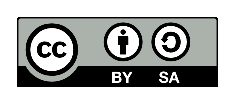
\includegraphics[scale=0.5]{img/cc-by-sa_88x31} \par
	{\footnotesize{This work is licensed under the Creative Commons Attribution-ShareAlike 4.0 International License. To view a copy of this license, visit \href{http://creativecommons.org/licenses/by-sa/4.0/}{http://creativecommons.org/licenses/by-sa/4.0/} or send a letter to Creative Commons, PO Box 1866, Mountain View, CA 94042, USA.}}\par
\medskip
\qrcode[hyperlink,height=1.5cm]{http://creativecommons.org/licenses/by-sa/4.0/}
\end{center}
\vspace*{\stretch{1}}
\newpage
 % Licence page
% Copyright 2018-2022 Pietro Prandini
% 
% This file is part of GuitarHub.
% 
% GuitarHub is free software: you can redistribute it and/or modify
% it under the terms of the GNU General Public License as published by
% the Free Software Foundation, either version 3 of the License, or
% (at your option) any later version.
% 
% GuitarHub is distributed in the hope that it will be useful,
% but WITHOUT ANY WARRANTY; without even the implied warranty of
% MERCHANTABILITY or FITNESS FOR A PARTICULAR PURPOSE.  See the
% GNU General Public License for more details.
% 
% You should have received a copy of the GNU General Public License
% along with GuitarHub.  If not, see <https://www.gnu.org/licenses/>.

\vspace*{\stretch{5}}
\section*{Preface}
The primary aim of this project is to create a printable guitar chords booklet for everyone.\par
\medskip
This booklet provides a lot of possibilities: you can update it with new songs without reprinting the whole book,
you can share this booklet with your friends, you can use it for bringing the music to every street of the world, or rather, you can become a GuitarHub hero.\par
\medskip
Thank you for using this booklet.\par
\smallskip
Thank you for sharing it.\par
\smallskip
Thank you for becoming a GuitarHub hero.\par
\bigskip
\begin{flushright}
	{\small{\textit{The first author of this booklet,}}}\par
	\medskip
	{\large{\textit{\rmfamily Pietro Prandini}}}\par
\end{flushright}
\vspace*{\stretch{12}}
\newpage

% Copyright 2018-2023 Pietro Prandini
%
% This file is part of GuitarHub.
%
% GuitarHub is free software: you can redistribute it and/or modify
% it under the terms of the GNU General Public License as published by
% the Free Software Foundation, either version 3 of the License, or
% (at your option) any later version.
%
% GuitarHub is distributed in the hope that it will be useful,
% but WITHOUT ANY WARRANTY; without even the implied warranty of
% MERCHANTABILITY or FITNESS FOR A PARTICULAR PURPOSE.  See the
% GNU General Public License for more details.
%
% You should have received a copy of the GNU General Public License
% along with GuitarHub.  If not, see <https://www.gnu.org/licenses/>.

\section*{Considerations}
This book is meant mainly for the guitar players who would like to have a chords book that is updated periodically without the loss of formatting and any other related problems.\par
It is highly recommended to print the content of this booklet and put it in a ring notebook - when a new song is added you can print it out and place it in a desired location. In order to avoid inconsistencies when adding the new songs to your collection, the pages are not labeled with any numbers. You can, for example, order the songs alphabetically.\par

\section*{Features}
\begin{itemize}
\item The booklet is available to be printed at once, including all the songs till date and then you can expand it by adding the newly released songs without the necessity to reprint the whole booklet;
\item the format of a single page is ISO A5 which supports the idea of  portability;
\item creating songs with musical note names in both absolute and solfege systems and providing the lyrics at the same time;
\item easy and automatic transposition of the chords;
\item ability to add your favourite songs;
\item the book is licensed by a Free Culture License;
\item support for creating songs;
\item support for generating the booklets.
\end{itemize}

\section*{How to have a copy}
See \href{https://github.com/PietroPrandini/GuitarHub}{https://github.com/PietroPrandini/GuitarHub}

\begin{center}
  \qrcode[hyperlink,height=1.5cm]{https://github.com/PietroPrandini/GuitarHub}
\end{center}
\newpage


%	Indexes
\checkodd
%\showindex[2]{Chords}{chords}
%\showindex[2]{Canti per la Liturgia, per le Celebrazioni e per la Preghiera}{chiesa}
%\showindex[2]{Jukebox}{jukebox}
%\showindex[2]{Christmas}{christmas}

%	Showing the lists of the songs
%{\makeatletter\def\SB@ellipspread#1#2{\begin{flushleft}- #1\par\end{flushleft}}\showindex[2]{Chords}{chords}}
{\makeatletter\def\SB@ellipspread#1#2{- #1\hspace*{\fill}\par}\showindex[2]{Canti per la Liturgia, per le Celebrazioni e per la Preghiera\\\tiny{ \filemodprintdate{"tex/songsChapters/chiesa.tex"} }}{chiesa}}
{\makeatletter\def\SB@ellipspread#1#2{- #1\hspace*{\fill}\par}\showindex[2]{Jukebox\\\tiny{ \filemodprintdate{"tex/songsChapters/jukebox.tex"} }}{jukebox}}
{\makeatletter\def\SB@ellipspread#1#2{- #1\hspace*{\fill}\par}\showindex[2]{Christmas\\\tiny{ \filemodprintdate{"tex/songsChapters/christmas.tex"} }}{christmas}}
\ifchorded
%	New chapter
%	Start on a right page and the title is in a blank page
\checkodd
\vspace*{\stretch{3}}
\songchapter{Chords}
\vspace*{\stretch{5}}
\newpage
%	Songs of this chapter
\songpos{0}
\begin{songs}{chords}
	% Copyright 2018-2022 Pietro Prandini
%
% This file is part of GuitarHub.
%
% GuitarHub is free software: you can redistribute it and/or modify
% it under the terms of the GNU General Public License as published by
% the Free Software Foundation, either version 3 of the License, or
% (at your option) any later version.
%
% GuitarHub is distributed in the hope that it will be useful,
% but WITHOUT ANY WARRANTY; without even the implied warranty of
% MERCHANTABILITY or FITNESS FOR A PARTICULAR PURPOSE.  See the
% GNU General Public License for more details.
%
% You should have received a copy of the GNU General Public License
% along with GuitarHub.  If not, see <https://www.gnu.org/licenses/>.

% Copyright 2018-2021 Pietro Prandini
%
% This file is part of GuitarHub.
%
% GuitarHub is free software: you can redistribute it and/or modify
% it under the terms of the GNU General Public License as published by
% the Free Software Foundation, either version 3 of the License, or
% (at your option) any later version.
%
% GuitarHub is distributed in the hope that it will be useful,
% but WITHOUT ANY WARRANTY; without even the implied warranty of
% MERCHANTABILITY or FITNESS FOR A PARTICULAR PURPOSE.  See the
% GNU General Public License for more details.
%
% You should have received a copy of the GNU General Public License
% along with GuitarHub.  If not, see <https://www.gnu.org/licenses/>.

\beginsong{Guitar chords}[
,cr={\centering{\href{https://github.com/PietroPrandini/GuitarHub}{https://github.com/PietroPrandini/GuitarHub}\\\href{http://creativecommons.org/licenses/by-sa/4.0/}{\textbf{CC BY-SA}} 2018-2021 Pietro Prandini}}
]

\vspace*{\stretch{3}}

\begin{center}
\hspace*{\fill}
\gtab{A}{X02220:002340}\hspace*{\fill}
\gtab{A#/B&}{(X13331):112341}\hspace*{\fill}
\gtab{B}{(X24442):112341}\hspace*{\fill}
\gtab{C}{X32010:032010}\hspace*{\fill}
\gtab{C#/D&}{4:(X13331):112341}\hspace*{\fill}
\gtab{D}{XX0232:000132}
\hspace*{\fill}\par

\vspace*{\stretch{2}}

\hspace*{\fill}
\gtab{D#/E&}{6:(X13331):112341}\hspace*{\fill}
\gtab{E}{022100:023100}\hspace*{\fill}
\gtab{F}{(133211):134211}\hspace*{\fill}
\gtab{F#/G&}{(244322):134211}\hspace*{\fill}
\gtab{G}{320033:210034}\hspace*{\fill}
\gtab{G#/A&}{4:(133211):134211}
\hspace*{\fill}\par

\vspace*{\stretch{4}}

\hspace*{\fill}
\gtab{Am}{X02210:002310}\hspace*{\fill}
\gtab{A#m/B&m}{(X13321):113421}\hspace*{\fill}
\gtab{Bm}{(X24432):113421}\hspace*{\fill}
\gtab{Cm}{3:(X13321):113421}\hspace*{\fill}
\gtab{C#m/D&m}{4:(X13321):113421}\hspace*{\fill}
\gtab{Dm}{XX0231:000241}
\hspace*{\fill}\par

\vspace*{\stretch{2}}

\hspace*{\fill}
\gtab{D#m/E&m}{6:(X13321):113421}\hspace*{\fill}
\gtab{Em}{022000:023000}\hspace*{\fill}
\gtab{Fm}{(133111):134111}\hspace*{\fill}
\gtab{F#m/G&m}{(244222):134111}\hspace*{\fill}
\gtab{Gm}{3:(133111):134111}\hspace*{\fill}
\gtab{G#m/A&m}{4:(133111):134111}
\hspace*{\fill}\par
\end{center}

\vspace*{\stretch{3}}

\endsong
\newsongpage
% Copyright 2018-2023 Pietro Prandini
%
% This file is part of GuitarHub.
%
% GuitarHub is free software: you can redistribute it and/or modify
% it under the terms of the GNU General Public License as published by
% the Free Software Foundation, either version 3 of the License, or
% (at your option) any later version.
%
% GuitarHub is distributed in the hope that it will be useful,
% but WITHOUT ANY WARRANTY; without even the implied warranty of
% MERCHANTABILITY or FITNESS FOR A PARTICULAR PURPOSE.  See the
% GNU General Public License for more details.
%
% You should have received a copy of the GNU General Public License
% along with GuitarHub.  If not, see <https://www.gnu.org/licenses/>.

\beginsong{Ukulele chords}[
,cr={\centering{\href{https://github.com/PietroPrandini/GuitarHub}{https://github.com/PietroPrandini/GuitarHub}\\\href{http://creativecommons.org/licenses/by-sa/4.0/}{\textbf{CC BY-SA}} 2018-2023 Pietro Prandini}}
]

\vspace*{\stretch{3}}

\begin{center}

\hspace*{\fill}
\gtab{A}{2100:2100}\hspace*{\fill}
\gtab{A#/B&}{(3211):3211}\hspace*{\fill}
\gtab{B}{(4322):3211}\hspace*{\fill}
\gtab{C}{0003:0003}\hspace*{\fill}
\gtab{C#/D&}{(1114):1114}\hspace*{\fill}
\gtab{D}{2220:1230}
\hspace*{\fill}\par

\vspace*{\stretch{2}}

\hspace*{\fill}
\gtab{D#/E&}{0331:0341}\hspace*{\fill}
\gtab{E}{4442:2341}\hspace*{\fill}
\gtab{F}{2010:2010}\hspace*{\fill}
\gtab{F#/G&}{(3121):3121}\hspace*{\fill}
\gtab{G}{0232:0132}\hspace*{\fill}
\gtab{G#/A&}{3:(3121):3121}
\hspace*{\fill}

\vspace*{\stretch{4}}

\hspace*{\fill}
\gtab{Am}{2000:2000}\hspace*{\fill}
\gtab{A#m/B&m}{(3111):3111}\hspace*{\fill}
\gtab{Bm}{(4222):3111}\hspace*{\fill}
\gtab{Cm}{0(333):0111}\hspace*{\fill}
\gtab{C#m/D&m}{1104:1204}\hspace*{\fill}
\gtab{Dm}{2210:2310}
\hspace*{\fill}\par

\vspace*{\stretch{2}}

\hspace*{\fill}
\gtab{D#m/E&m}{3321:3421}\hspace*{\fill}
\gtab{Em}{0432:0321}\hspace*{\fill}
\gtab{Fm}{1013:1024}\hspace*{\fill}
\gtab{F#m/G&m}{2120:2130}\hspace*{\fill}
\gtab{Gm}{0231:0231}\hspace*{\fill}
\gtab{G#m/A&m}{4342:3241}
\hspace*{\fill}\par
\end{center}

\vspace*{\stretch{3}}

\endsong
\newsongpage

\end{songs}
\songpos{3}
\fi

%	New chapter
%	Start on a right page and the title is in a blank page
\checkodd
\vspace*{\stretch{3}}
\songchapter{Canti per la Liturgia, per le Celebrazioni e per la Preghiera}
\vspace*{\stretch{5}}
\newpage
%	Songs of this chapter
\begin{songs}{chiesa}
	%	Songs of the chiesa chapter
\scleardpage
% Copyright 2018-2023 Pietro Prandini
%
% This file is part of GuitarHub.
%
% GuitarHub is free software: you can redistribute it and/or modify
% it under the terms of the GNU General Public License as published by
% the Free Software Foundation, either version 3 of the License, or
% (at your option) any later version.
%
% GuitarHub is distributed in the hope that it will be useful,
% but WITHOUT ANY WARRANTY; without even the implied warranty of
% MERCHANTABILITY or FITNESS FOR A PARTICULAR PURPOSE.  See the
% GNU General Public License for more details.
%
% You should have received a copy of the GNU General Public License
% along with GuitarHub.  If not, see <https://www.gnu.org/licenses/>.

\begin{twocolssong}
\beginsong{Adesso è la pienezza}[
,cr={\centering{\href{https://github.com/PietroPrandini/GuitarHub}{https://github.com/PietroPrandini/GuitarHub}\\\href{http://creativecommons.org/licenses/by-sa/4.0/}{\textbf{CC BY-SA}} 2018-2023 Pietro Prandini}}
]

\transpose{0}

% Copyright 2018-2023 Pietro Prandini
%
% This file is part of GuitarHub.
%
% GuitarHub is free software: you can redistribute it and/or modify
% it under the terms of the GNU General Public License as published by
% the Free Software Foundation, either version 3 of the License, or
% (at your option) any later version.
%
% GuitarHub is distributed in the hope that it will be useful,
% but WITHOUT ANY WARRANTY; without even the implied warranty of
% MERCHANTABILITY or FITNESS FOR A PARTICULAR PURPOSE.  See the
% GNU General Public License for more details.
%
% You should have received a copy of the GNU General Public License
% along with GuitarHub.  If not, see <https://www.gnu.org/licenses/>.

\begin{twocolssong}
\beginsong{Adesso è la pienezza}[
,cr={\centering{\href{https://github.com/PietroPrandini/GuitarHub}{https://github.com/PietroPrandini/GuitarHub}\\\href{http://creativecommons.org/licenses/by-sa/4.0/}{\textbf{CC BY-SA}} 2018-2023 Pietro Prandini}}
]

\transpose{0}

\input{"tex/songs/Adesso e la pienezza.tex"}

\endsong
\end{twocolssong}


\endsong
\end{twocolssong}

\ifchorded
	\scleardpage
	% Copyright 2018-2021 Pietro Prandini
% 
% This file is part of GuitarHub.
% 
% GuitarHub is free software: you can redistribute it and/or modify
% it under the terms of the GNU General Public License as published by
% the Free Software Foundation, either version 3 of the License, or
% (at your option) any later version.
% 
% GuitarHub is distributed in the hope that it will be useful,
% but WITHOUT ANY WARRANTY; without even the implied warranty of
% MERCHANTABILITY or FITNESS FOR A PARTICULAR PURPOSE.  See the
% GNU General Public License for more details.
% 
% You should have received a copy of the GNU General Public License
% along with GuitarHub.  If not, see <https://www.gnu.org/licenses/>.

\beginsong{Adesso è la pienezza}[
,cr={\centering{\href{https://github.com/PietroPrandini/GuitarHub}{https://github.com/PietroPrandini/GuitarHub}\\\href{http://creativecommons.org/licenses/by-sa/4.0/}{\textbf{CC BY-SA}} 2018-2021 Pietro Prandini}}
]

\transpose{10} 

% Copyright 2018-2023 Pietro Prandini
%
% This file is part of GuitarHub.
%
% GuitarHub is free software: you can redistribute it and/or modify
% it under the terms of the GNU General Public License as published by
% the Free Software Foundation, either version 3 of the License, or
% (at your option) any later version.
%
% GuitarHub is distributed in the hope that it will be useful,
% but WITHOUT ANY WARRANTY; without even the implied warranty of
% MERCHANTABILITY or FITNESS FOR A PARTICULAR PURPOSE.  See the
% GNU General Public License for more details.
%
% You should have received a copy of the GNU General Public License
% along with GuitarHub.  If not, see <https://www.gnu.org/licenses/>.

\begin{twocolssong}
\beginsong{Adesso è la pienezza}[
,cr={\centering{\href{https://github.com/PietroPrandini/GuitarHub}{https://github.com/PietroPrandini/GuitarHub}\\\href{http://creativecommons.org/licenses/by-sa/4.0/}{\textbf{CC BY-SA}} 2018-2023 Pietro Prandini}}
]

\transpose{0}

\input{"tex/songs/Adesso e la pienezza.tex"}

\endsong
\end{twocolssong}


\endsong


\fi
\scleardpage
\input{"tex/songsChapters/chiesa/Adoro Te"}
\scleardpage
%	Uncomment the next two lines and the last twice
%	if the song is over 2 pages
%\renewcommand{\lyricfont}{\sffamily\small}
%\renewcommand{\printchord}[1]{\rmfamily\bf#1\small}

\beginsong{%Title
Alleluia la Tua festa}[
%by={} % Authors, composers, and other contributors
%,cr={} % Copyright information
%,li={} % Licensing information
%,sr={} % Related scripture references
%,index={} % An extra index entry for a line of lyrics
%,ititle={} % An extra index entry for a hidden title
]

%\capo{0}
\transpose{0} % Autoimatic transpositions from +0 to +12 semitones
%\meter{4}{4}

%	\ifchorded
%	\beginverse* % * not count the verse
%		{\nolyrics Intro: }
%	\endverse
%	\fi

	\beginchorus
		%chorus
		\[C]Alle\[F]luia, alleluia,
		\[C]alle\[G]luia, alleluia.
		\[C]Alle\[F]luia, alleluia,
		\[C]al\[G]lelu\[C]ia. \rep{2}
	\endchorus

	\beginverse*\memorize % \memorize is used to set the chords you would like to use with ^ in the next verses
		%verse
		\[C]La Tua \[F]festa non \[G]deve \[C]finire,
		non \[Am]deve fi\[Dm]nire e \[G]non fini\[C]rà.
		\[C]La Tua \[F]festa non \[G]deve \[C]finire,
		non \[Am]deve fi\[Dm]nire e \[G]non fini\[C]rà. \[C7]
		Per\[F]chè la \[G]festa \[C]siamo \[Am]noi
		che \[F]cammi\[G]niamo verso \[C]Te, \[C7]
		per\[F]chè la \[G]festa \[C]siamo \[Am]noi
		can\[D7]tando insieme co\[G4]sì. \[G]
	\endverse

%	\ifchorded
%	\beginverse* % * not count the verse
%		{\nolyrics Strum: }
%	\endverse
%	\fi

%	\textnote{} % Notes for both lyric and chorded songs
%	\musicnote{} % Notes visible only in chorded books (not visible in lyric mode)
%	\rep{n} % Repeat n times
%	\lrep ... \rrep \rep{n} % margins of the repeat

%	Writing chords
%
% Alphabetic note names:     A      B      C      D      E      F      G
% Solfedge note names:       LA     SI     DO     RE     MI     FA     SOL
%
%	Compatible notation:
%
% Naturals:                  \[A]   \[B]   \[C]   \[D]   \[E]   \[F]   \[G]
% Flat (Bemolle):            \[A&]  \[B&]  \[C&]  \[D&]  \[E&]  \[F&]  \[G&]
% Sharp (Diesis):            \[A#]  \[B#]  \[C#]  \[D#]  \[E#]  \[F#]  \[G#]
% Minor:                     \[Am]  \[Bm]  \[Cm]  \[Dm]  \[Em]  \[Fm]  \[Gm]
% Flat and minor:            \[A&m] \[B&m] \[C&m] \[D&m] \[E&m] \[F&m] \[G&m]
% Sharp and minor:           \[A#m] \[B#m] \[C#m] \[D#m] \[E#m] \[F#m] \[G#m]

\endsong

%\renewcommand{\lyricfont}{\sffamily}
%\renewcommand{\printchord}[1]{\rmfamily\bf#1}

\scleardpage
%	Uncomment the next two lines and the last twice
%	if the song is over 2 pages
%\renewcommand{\lyricfont}{\sffamily\small}
%\renewcommand{\printchord}[1]{\rmfamily\bf#1\small}

\beginsong{%Title
Alleluia passeranno i cieli}[
%by={} % Authors, composers, and other contributors
cr={\centering{\href{https://github.com/PietroPrandini/GuitarHub}{https://github.com/PietroPrandini/GuitarHub} \href{http://creativecommons.org/licenses/by-sa/4.0/}{CC-BY-SA} \filemodprintdate{\jobname}}}
%,sr={} % Related scripture references
%,index={} % An extra index entry for a line of lyrics
%,ititle={} % An extra index entry for a hidden title
]

%\capo{0}
\transpose{0} % Automatic transpositions from +0 to +12 semitones
%\meter{4}{4}

	\ifchorded
	\beginverse* % * not count the verse
		{\nolyrics Intro: \[D] \[A] \rep{2}}
	\endverse
	\fi

	\beginchorus
		\[D]Alle\[A]luia, \[F#m]
		\[Bm]alleluia, \[F#m]alleluia,
		\[G]alleluia, \[D]allelu\[Em]ia, \[A]
		\[D]alle\[G]luia, al\[A]lelu\[D]ia.
	\endchorus

	\beginverse*
		\[D]Passeranno i \[A]cieli \[F#m]
		e \[Bm]passerà la \[F#m]terra,
		\[G]la Sua Parola \[D]non passe\[Em]rà, \[A]
		\[D]alle\[G]luia, al\[A]lelu\[D]ia.
	\endverse

%	\ifchorded
%	\beginverse* % * not count the verse
%		{\nolyrics Strum: }
%	\endverse
%	\fi

%	\textnote{} % Notes for both lyric and chorded songs
%	\musicnote{} % Notes visible only in chorded books (not visible in lyric mode)
%	\rep{n} % Repeat n times
%	\lrep ... \rrep \rep{n} % margins of the repeat

%	Writing chords
%
% Alphabetic note names:     A      B      C      D      E      F      G
% Solfedge note names:       LA     SI     DO     RE     MI     FA     SOL
%
%	Compatible notation:
%
% Naturals:                  \[A]   \[B]   \[C]   \[D]   \[E]   \[F]   \[G]
% Flat (Bemolle):            \[A&]  \[B&]  \[C&]  \[D&]  \[E&]  \[F&]  \[G&]
% Sharp (Diesis):            \[A#]  \[B#]  \[C#]  \[D#]  \[E#]  \[F#]  \[G#]
% Minor:                     \[Am]  \[Bm]  \[Cm]  \[Dm]  \[Em]  \[Fm]  \[Gm]
% Flat and minor:            \[A&m] \[B&m] \[C&m] \[D&m] \[E&m] \[F&m] \[G&m]
% Sharp and minor:           \[A#m] \[B#m] \[C#m] \[D#m] \[E#m] \[F#m] \[G#m]

\endsong

%\renewcommand{\lyricfont}{\sffamily}
%\renewcommand{\printchord}[1]{\rmfamily\bf#1}

\scleardpage
\beginsong{Alleluia questa Tua parola}[
cr={\centering{\href{https://github.com/PietroPrandini/GuitarHub}{https://github.com/PietroPrandini/GuitarHub} \href{http://creativecommons.org/licenses/by-sa/4.0/}{CC-BY-SA} \filemodprintdate{\jobname}}}
]
\transpose{0}
%{\nolyrics Intro: }

\ifchorded
\beginverse*
{\nolyrics Intro: \[D] \[Em] \[G] \[D]}
\endverse
\fi

\beginchorus
\[D]Alleluia, \[A]Alleluia, \[Bm]Alleluia, A\[F#]lleluia,
\[G]Alleluia, \[D]Alleluia, \[E]Alleluia, A\[A4]lle\[A]luia.
\[D]Alleluia, \[A]Alleluia, \[Bm]Alleluia, A\[F#]lleluia,
\[G]Alleluia, \[D]Alleluia, \[E]Alleluia, A\[A4]lle\[A]lui\[D]a.
\endchorus

\beginverse*
\[D]Questa Tua parola \[C]non avr\`a mai fine,
\[G]ha varcato i cieli e \[D]porter\`a i suoi frutti.
\[D]Questa Tua parola \[C]non avr\`a mai fine,
\[G]ha varcato i cieli e \[A4]porter\`a i suoi \[A7]frutti.
\endverse

\beginchorus
\[D]Alleluia, \[A]Alleluia, \[Bm]Alleluia, A\[F#]lleluia,
\[G]Alleluia, \[D]Alleluia, \[E]Alleluia, A\[A4]lle\[A]lui\[D]a.
\endchorus

\endsong

\scleardpage
% Copyright 2018-2021 Pietro Prandini
% 
% This file is part of GuitarHub.
% 
% GuitarHub is free software: you can redistribute it and/or modify
% it under the terms of the GNU General Public License as published by
% the Free Software Foundation, either version 3 of the License, or
% (at your option) any later version.
% 
% GuitarHub is distributed in the hope that it will be useful,
% but WITHOUT ANY WARRANTY; without even the implied warranty of
% MERCHANTABILITY or FITNESS FOR A PARTICULAR PURPOSE.  See the
% GNU General Public License for more details.
% 
% You should have received a copy of the GNU General Public License
% along with GuitarHub.  If not, see <https://www.gnu.org/licenses/>.

\beginsong{Alleluia servire è}[
,cr={\centering{\href{https://github.com/PietroPrandini/GuitarHub}{https://github.com/PietroPrandini/GuitarHub}\\\href{http://creativecommons.org/licenses/by-sa/4.0/}{\textbf{CC BY-SA}} 2018-2021 Pietro Prandini}}
]

\transpose{0} 

% Copyright 2018-2021 Pietro Prandini
% 
% This file is part of GuitarHub.
% 
% GuitarHub is free software: you can redistribute it and/or modify
% it under the terms of the GNU General Public License as published by
% the Free Software Foundation, either version 3 of the License, or
% (at your option) any later version.
% 
% GuitarHub is distributed in the hope that it will be useful,
% but WITHOUT ANY WARRANTY; without even the implied warranty of
% MERCHANTABILITY or FITNESS FOR A PARTICULAR PURPOSE.  See the
% GNU General Public License for more details.
% 
% You should have received a copy of the GNU General Public License
% along with GuitarHub.  If not, see <https://www.gnu.org/licenses/>.

\beginsong{Alleluia servire è}[
,cr={\centering{\href{https://github.com/PietroPrandini/GuitarHub}{https://github.com/PietroPrandini/GuitarHub}\\\href{http://creativecommons.org/licenses/by-sa/4.0/}{\textbf{CC BY-SA}} 2018-2021 Pietro Prandini}}
]

\transpose{0} 

\input{"tex/songs/Alleluia servire e.tex"}

\endsong



\endsong


\scleardpage
% Copyright 2018-2021 Pietro Prandini
% 
% This file is part of GuitarHub.
% 
% GuitarHub is free software: you can redistribute it and/or modify
% it under the terms of the GNU General Public License as published by
% the Free Software Foundation, either version 3 of the License, or
% (at your option) any later version.
% 
% GuitarHub is distributed in the hope that it will be useful,
% but WITHOUT ANY WARRANTY; without even the implied warranty of
% MERCHANTABILITY or FITNESS FOR A PARTICULAR PURPOSE.  See the
% GNU General Public License for more details.
% 
% You should have received a copy of the GNU General Public License
% along with GuitarHub.  If not, see <https://www.gnu.org/licenses/>.

%	Uncomment the next two lines and the last twice
%	if the song is over 2 pages
%\renewcommand{\lyricfont}{\small}
%\renewcommand{\printchord}[1]{\bf#1\small}

\beginsong{%Title
Alleluia Signore sei venuto}[
%by={} % Authors, composers, and other contributors
,cr={\centering{\href{https://github.com/PietroPrandini/GuitarHub}{https://github.com/PietroPrandini/GuitarHub}\\\href{http://creativecommons.org/licenses/by-sa/4.0/}{\textbf{CC BY-SA}} 2018-2021 Pietro Prandini}}, % Copyright information
%,sr={} % Related scripture references
%,index={} % An extra index entry for a line of lyrics
%,ititle={} % An extra index entry for a hidden title
]

%\capo{0}
\transpose{0} % Automatic transpositions from +0 to +12 semitones

% Copyright 2018-2021 Pietro Prandini
% 
% This file is part of GuitarHub.
% 
% GuitarHub is free software: you can redistribute it and/or modify
% it under the terms of the GNU General Public License as published by
% the Free Software Foundation, either version 3 of the License, or
% (at your option) any later version.
% 
% GuitarHub is distributed in the hope that it will be useful,
% but WITHOUT ANY WARRANTY; without even the implied warranty of
% MERCHANTABILITY or FITNESS FOR A PARTICULAR PURPOSE.  See the
% GNU General Public License for more details.
% 
% You should have received a copy of the GNU General Public License
% along with GuitarHub.  If not, see <https://www.gnu.org/licenses/>.

%	Uncomment the next two lines and the last twice
%	if the song is over 2 pages
%\renewcommand{\lyricfont}{\small}
%\renewcommand{\printchord}[1]{\bf#1\small}

\beginsong{%Title
Alleluia Signore sei venuto}[
%by={} % Authors, composers, and other contributors
,cr={\centering{\href{https://github.com/PietroPrandini/GuitarHub}{https://github.com/PietroPrandini/GuitarHub}\\\href{http://creativecommons.org/licenses/by-sa/4.0/}{\textbf{CC BY-SA}} 2018-2021 Pietro Prandini}}, % Copyright information
%,sr={} % Related scripture references
%,index={} % An extra index entry for a line of lyrics
%,ititle={} % An extra index entry for a hidden title
]

%\capo{0}
\transpose{0} % Automatic transpositions from +0 to +12 semitones

\input{"tex/songs/Alleluia Signore sei venuto.tex"}

\endsong

%\renewcommand{\lyricfont}{}
%\renewcommand{\printchord}[1]{\bf#1}


\endsong

%\renewcommand{\lyricfont}{}
%\renewcommand{\printchord}[1]{\bf#1}

\ifchorded
	\scleardpage
	% Copyright 2018-2022 Pietro Prandini
% 
% This file is part of GuitarHub.
% 
% GuitarHub is free software: you can redistribute it and/or modify
% it under the terms of the GNU General Public License as published by
% the Free Software Foundation, either version 3 of the License, or
% (at your option) any later version.
% 
% GuitarHub is distributed in the hope that it will be useful,
% but WITHOUT ANY WARRANTY; without even the implied warranty of
% MERCHANTABILITY or FITNESS FOR A PARTICULAR PURPOSE.  See the
% GNU General Public License for more details.
% 
% You should have received a copy of the GNU General Public License
% along with GuitarHub.  If not, see <https://www.gnu.org/licenses/>.

\beginsong{Alleluia Signore sei venuto}[
,cr={\centering{\href{https://github.com/PietroPrandini/GuitarHub}{https://github.com/PietroPrandini/GuitarHub}\\\href{http://creativecommons.org/licenses/by-sa/4.0/}{\textbf{CC BY-SA}} 2018-2022 Pietro Prandini}}
]

\transpose{10} 

% Copyright 2018-2021 Pietro Prandini
% 
% This file is part of GuitarHub.
% 
% GuitarHub is free software: you can redistribute it and/or modify
% it under the terms of the GNU General Public License as published by
% the Free Software Foundation, either version 3 of the License, or
% (at your option) any later version.
% 
% GuitarHub is distributed in the hope that it will be useful,
% but WITHOUT ANY WARRANTY; without even the implied warranty of
% MERCHANTABILITY or FITNESS FOR A PARTICULAR PURPOSE.  See the
% GNU General Public License for more details.
% 
% You should have received a copy of the GNU General Public License
% along with GuitarHub.  If not, see <https://www.gnu.org/licenses/>.

%	Uncomment the next two lines and the last twice
%	if the song is over 2 pages
%\renewcommand{\lyricfont}{\small}
%\renewcommand{\printchord}[1]{\bf#1\small}

\beginsong{%Title
Alleluia Signore sei venuto}[
%by={} % Authors, composers, and other contributors
,cr={\centering{\href{https://github.com/PietroPrandini/GuitarHub}{https://github.com/PietroPrandini/GuitarHub}\\\href{http://creativecommons.org/licenses/by-sa/4.0/}{\textbf{CC BY-SA}} 2018-2021 Pietro Prandini}}, % Copyright information
%,sr={} % Related scripture references
%,index={} % An extra index entry for a line of lyrics
%,ititle={} % An extra index entry for a hidden title
]

%\capo{0}
\transpose{0} % Automatic transpositions from +0 to +12 semitones

\input{"tex/songs/Alleluia Signore sei venuto.tex"}

\endsong

%\renewcommand{\lyricfont}{}
%\renewcommand{\printchord}[1]{\bf#1}


\endsong


\fi
\scleardpage
%	Uncomment the next two lines and the last twice
%	if the song is over 2 pages
%\renewcommand{\lyricfont}{\small}
%\renewcommand{\printchord}[1]{\bf#1\small}

\beginsong{%Title
Alleluia, una luce splendida}[
by={F. Buttazzo} % Authors, composers, and other contributors
,cr={\centering{\href{https://github.com/PietroPrandini/GuitarHub}{https://github.com/PietroPrandini/GuitarHub}\\\href{http://creativecommons.org/licenses/by-sa/4.0/}{\textbf{CC BY-SA}} 2018-2021 Pietro Prandini}}, % Copyright information
%,li={} % Licensing information
%,sr={} % Related scripture references
%,index={} % An extra index entry for a line of lyrics
%,ititle={} % An extra index entry for a hidden title
]

%\capo{0}
\transpose{0} % Automatic transpositions from +0 to +12 semitones

%	Uncomment the next two lines and the last twice
%	if the song is over 2 pages
%\renewcommand{\lyricfont}{\small}
%\renewcommand{\printchord}[1]{\bf#1\small}

\beginsong{%Title
Alleluia, una luce splendida}[
by={F. Buttazzo} % Authors, composers, and other contributors
,cr={\centering{\href{https://github.com/PietroPrandini/GuitarHub}{https://github.com/PietroPrandini/GuitarHub}\\\href{http://creativecommons.org/licenses/by-sa/4.0/}{\textbf{CC BY-SA}} 2018-2021 Pietro Prandini}}, % Copyright information
%,li={} % Licensing information
%,sr={} % Related scripture references
%,index={} % An extra index entry for a line of lyrics
%,ititle={} % An extra index entry for a hidden title
]

%\capo{0}
\transpose{0} % Automatic transpositions from +0 to +12 semitones

\input{"tex/songs/Alleluia una luce splendida.tex"}

\endsong

%\renewcommand{\lyricfont}{}
%\renewcommand{\printchord}[1]{\bf#1}


\endsong

%\renewcommand{\lyricfont}{}
%\renewcommand{\printchord}[1]{\bf#1}

\ifchorded
	\scleardpage
	% Copyright 2018-2023 Pietro Prandini
% 
% This file is part of GuitarHub.
% 
% GuitarHub is free software: you can redistribute it and/or modify
% it under the terms of the GNU General Public License as published by
% the Free Software Foundation, either version 3 of the License, or
% (at your option) any later version.
% 
% GuitarHub is distributed in the hope that it will be useful,
% but WITHOUT ANY WARRANTY; without even the implied warranty of
% MERCHANTABILITY or FITNESS FOR A PARTICULAR PURPOSE.  See the
% GNU General Public License for more details.
% 
% You should have received a copy of the GNU General Public License
% along with GuitarHub.  If not, see <https://www.gnu.org/licenses/>.

\beginsong{Alleluia, una luce splendida}[
by={F. Buttazzo} 
,cr={\centering{\href{https://github.com/PietroPrandini/GuitarHub}{https://github.com/PietroPrandini/GuitarHub}\\\href{http://creativecommons.org/licenses/by-sa/4.0/}{\textbf{CC BY-SA}} 2018-2023 Pietro Prandini}}
]

\transpose{10} 

%	Uncomment the next two lines and the last twice
%	if the song is over 2 pages
%\renewcommand{\lyricfont}{\small}
%\renewcommand{\printchord}[1]{\bf#1\small}

\beginsong{%Title
Alleluia, una luce splendida}[
by={F. Buttazzo} % Authors, composers, and other contributors
,cr={\centering{\href{https://github.com/PietroPrandini/GuitarHub}{https://github.com/PietroPrandini/GuitarHub}\\\href{http://creativecommons.org/licenses/by-sa/4.0/}{\textbf{CC BY-SA}} 2018-2021 Pietro Prandini}}, % Copyright information
%,li={} % Licensing information
%,sr={} % Related scripture references
%,index={} % An extra index entry for a line of lyrics
%,ititle={} % An extra index entry for a hidden title
]

%\capo{0}
\transpose{0} % Automatic transpositions from +0 to +12 semitones

\input{"tex/songs/Alleluia una luce splendida.tex"}

\endsong

%\renewcommand{\lyricfont}{}
%\renewcommand{\printchord}[1]{\bf#1}


\endsong


\fi
\scleardpage
\beginsong{%Title
Alleluia Verbum panis}[
%by={} % Authors, composers, and other contributors
,cr={\centering{\href{https://github.com/PietroPrandini/GuitarHub}{https://github.com/PietroPrandini/GuitarHub} - \href{http://creativecommons.org/licenses/by-sa/4.0/}{CC-BY-SA} - \filemodprintdate{"tex/chiesa/Alleluia Verbum panis.tex"}}}, % Copyright information
%,sr={} % Related scripture references
%,index={} % An extra index entry for a line of lyrics
%,ititle={} % An extra index entry for a hidden title
]

%\capo{0}
\transpose{0} % Automatic transpositions from +0 to +12 semitones

%	\beginverse* % * not count the verse
%		{\nolyrics Intro: }
%	\endverse

%	\beginverse\memorize % \memorize is used to set the chords you would like to use with ^ in the next verses
		%verse
%	\endverse
	\meter{4}{4}
	\beginchorus
		%chorus
		|\[Bm]Alle\[A]lu\[D]ia alle\[Em]lui\[A]a
		\[Bm]alle\[A]lu\[D]ia alle\[Em]l\[F#m]u\[Bm]ia \rep{2}
	\endchorus

	\beginverse*
	\meter{2}{4}|\[Bm] Alleluia allelu\meter{4}{4}|ia all\[A]eluia \[Bm] all\[A]eluia|
		\[Em] all\[F#m]eluia \echo{\[G]all\[A]eluia}|
	\meter{2}{4}|\[Bm] Alleluia all\[A]elu\meter{4}{4}|\[Bm]ia all\[A]eluia \[Bm] all\[A]eluia|
		\[Em] all\[F#m]eluia \echo{\[G]all\[A]eluia}|
	\endverse

%	\textnote{} % Notes for both lyric and chorded songs
%	\musicnote{} % Notes visible only in chorded books (not visible in lyric mode)
%	\rep{n} % Repeat n times

%	Writing chords
%
% Alphabetic note names:     A      B      C      D      E      F      G
% Solfedge note names:       LA     SI     DO     RE     MI     FA     SOL
%
%	Compatible notation:
%
% Naturals:                  \[A]   \[B]   \[C]   \[D]   \[E]   \[F]   \[G]
% Flat (Bemolle):            \[A&]  \[B&]  \[C&]  \[D&]  \[E&]  \[F&]  \[G&]
% Sharp (Diesis):            \[A#]  \[B#]  \[C#]  \[D#]  \[E#]  \[F#]  \[G#]
% Minor:                     \[Am]  \[Bm]  \[Cm]  \[Dm]  \[Em]  \[Fm]  \[Gm]
% Flat and minor:            \[A&m] \[B&m] \[C&m] \[D&m] \[E&m] \[F&m] \[G&m]
% Sharp and minor:           \[A#m] \[B#m] \[C#m] \[D#m] \[E#m] \[F#m] \[G#m]

%	You can print the book with solfege note names
%	by uncomment a line of the GuitarChords.tex:
%	```
%	%  \notenamesin{A}{B}{C}{D}{E}{F}{G}
  \notenamesout{LA}{SI}{DO}{RE}{MI}{FA}{SOL}
 % Solfedge note names
%	```

\endsong

\scleardpage
% Copyright 2018-2022 Pietro Prandini
% 
% This file is part of GuitarHub.
% 
% GuitarHub is free software: you can redistribute it and/or modify
% it under the terms of the GNU General Public License as published by
% the Free Software Foundation, either version 3 of the License, or
% (at your option) any later version.
% 
% GuitarHub is distributed in the hope that it will be useful,
% but WITHOUT ANY WARRANTY; without even the implied warranty of
% MERCHANTABILITY or FITNESS FOR A PARTICULAR PURPOSE.  See the
% GNU General Public License for more details.
% 
% You should have received a copy of the GNU General Public License
% along with GuitarHub.  If not, see <https://www.gnu.org/licenses/>.

\ifchorded

  \beginverse* 
  {\nolyrics Intro: \[Dm] \[C] \[B&] \[A]}
  \endverse

\fi

\beginverse\memorize 
\[Dm]Nebbia e freddo, giorni lunghi e \[C]amari,
mentre il seme m\[Dm]uore.
\[F]Poi il prodigio, antico e sempre \[C]nuovo
del primo filo d'\[B&]erba, e nel \[F]vento
dell'es\[C]tate ond\[Dm]eggiano le \[F]spighe:
a\[C]vremo ancora \[A]pan\[D]e.
\endverse

\beginchorus
\[G]Bened\[D]ici, \[G]o \[D]Signore \[C]questa o\[G]fferta
che por\[A]tiamo a Te.
\[G]Facci \[D]uno, \[Bm]come il \[F#m]Pane \[E]che anche \[G]oggi
hai \[D]dato a noi.
\endchorus

\beginverse
^Nei filari, dopo il lungo ^inverno,
fremono le ^viti.
^La rugiada avvolge nel si^lenzio
i primi tralci ^verdi, poi i ^colori
dell'aut^unno, coi ^grappoli ^maturi:
a^vremo ancora ^vi^no.
\endverse


\ifchorded
	\scleardpage
	\beginsong{%Titles
Benedici o Signore
}[
%by={},%authors, composers, and other contributors
,cr={\centering{\href{https://github.com/PietroPrandini/GuitarHub}{https://github.com/PietroPrandini/GuitarHub} \href{http://creativecommons.org/licenses/by-sa/4.0/}{CC-BY-SA} \filemodprintdate{"tex/chiesa/Benedici o Signore -2 capo1.tex"}}}, % Copyright information
%sr={},%related scripture references
%index={V1},%an extra index entry for a line of lyrics
%ititle={V1}%an extra index entry for a hidden title
]

\capo{1}
\transpose{9}

\ifchorded
  \beginverse* % * not count the verse
	  {\nolyrics Intro: \[Dm] \[C] \[B&] \[A]}
  \endverse
\fi
	\beginverse\memorize % \memorize is used to set the chords you would like to use with ^ in the next verses
	%verse
	\[Dm]Nebbia e freddo, giorni lunghi e \[C]amari,
	mentre il seme m\[Dm]uore.
	\[F]Poi il prodigio, antico e sempre \[C]nuovo
	del primo filo d'\[B&]erba, e nel \[F]vento
	dell'es\[C]tate ond\[Dm]eggiano le \[F]spighe:
	a\[C]vremo ancora \[A]pan\[D]e.
	\endverse

	\beginchorus
	%chorus
	\[G]Bened\[D]ici, \[G]o \[D]Signore \[C]questa o\[G]fferta
	che por\[A]tiamo a Te.
	\[G]Facci \[D]uno, \[Bm]come il \[F#m]Pane \[E]che anche \[G]oggi
	hai \[D]dato a noi.
	\endchorus

	\beginverse
	^Nei filari, dopo il lungo ^inverno,
	fremono le ^viti.
	^La rugiada avvolge nel si^lenzio
	i primi tralci ^verdi, poi i ^colori
	dell'aut^unno, coi ^grappoli ^maturi:
	a^vremo ancora ^vi^no.
	\endverse
% \textnote{} %for notes

%                 Do     Re     Mi     Fa     Sol    La     Si
%Naturali:        \[C]   \[D]   \[E]   \[F]   \[G]   \[A]   \[B]
%Bemolli:         \[C&]  \[D&]  \[E&]  \[F&]  \[G&]  \[A&]  \[B&]
%Diesis:          \[C#]  \[D#]  \[E#]  \[F#]  \[G#]  \[A#]  \[B#]
%Minori:          \[Cm]  \[Dm]  \[Em]  \[Fm]  \[Gm]  \[Am]  \[Bm]
%Bemolli minori:  \[C&m] \[D&m] \[E&m] \[F&m] \[G&m] \[A&m] \[B&m]
%Diesis minori:   \[C#m] \[D#m] \[E#m] \[F#m] \[G#m] \[A#m] \[B#m]

\endsong

\fi
\scleardpage
\beginsong{%Title
Canto dell'Amore}[
%by={} % Authors, composers, and other contributors
cr={\centering{\href{https://github.com/PietroPrandini/GuitarHub}{https://github.com/PietroPrandini/GuitarHub} \href{http://creativecommons.org/licenses/by-sa/4.0/}{CC-BY-SA} \filemodprintdate{\jobname}}}
%,sr={} % Related scripture references
%,index={} % An extra index entry for a line of lyrics
%,ititle={} % An extra index entry for a hidden title
]

%\capo{0}
\transpose{0} % Automatic transpositions from +0 to +12 semitones

%	\beginverse* % * not count the verse
%		{\nolyrics Intro: }
%	\endverse

	\beginverse\memorize % \memorize is used to set the chords you would like to use with ^ in the next verses
		%verse
		Se \[E]dovrai attraversare il de\[C#m]serto
		non te\[A]mere Io sarò con \[E]te
		se dovrai camminare nel f\[C#m]uoco
		la sua f\[A]iamma non ti bruce\[E]rà
		segui\[B]rai la mia \[A]luce nella \[E]notte
		senti\[F#m]rai la mia \[B]forza nel camm\[C#m]ino
		io \[D]sono il tuo Dio, \[A] il Signore\[E]. \[C#m] \[A] \[E]
	\endverse

	\beginverse
		Sono ^Io che ti ho fatto e plas^mato
		ti ho ch^iamato per nome^
		Io da sempre ti ho conosc^iuto
		e ti ho ^dato il mio amore^
		perché ^tu sei pre^zioso ai miei oc^chi
		vali ^più del ^più grande dei te^sori
		Io ^sarò con te ^ dovunque and^rai. ^ ^ ^
	\endverse

	\ifchorded
	\beginverse*
		{\nolyrics Bridge \[B] \[A] \[E] \[D] \[A] \[B]}
	\endverse
	\fi

	\beginverse
		Non pen^sare alle cose di ^ieri
		cose n^uove fioriscono ^già
		aprirò nel deserto sent^ieri
		darò ^acqua nell'aridi^tà
		perché ^tu sei pre^zioso ai miei oc^chi
		vali ^più del ^più grande dei te^sori
		io ^sarò con te^ dovunque and^rai
		perché \[B]tu sei pre\[A]zioso ai miei oc\[E]chi
		vali \[F#m]più del \[B]più grande dei te\[C#m]sori
		io \[D]sarò con te \[A] dovunque and\[E]rai. \[C#m] \[A] \[E]
	\endverse

	\beginverse*
		Io ti sarò \[C#m] accanto \[A]sarò con \[E]te
		per tutto \[C#m] il tuo viaggio \[A]sarò con \[E]te. \rep{2}
	\endverse

%	\beginchorus
		%chorus
%	\endchorus

%	\textnote{} % Notes for both lyric and chorded songs
%	\musicnote{} % Notes visible only in chorded books (not visible in lyric mode)
%	\rep{n} % Repeat n times

%	Writing chords
%
% Alphabetic note names:     A      B      C      D      E      F      G
% Solfedge note names:       LA     SI     DO     RE     MI     FA     SOL
%
%	Compatible notation:
%
% Naturals:                  \[A]   \[B]   \[C]   \[D]   \[E]   \[F]   \[G]
% Flat (Bemolle):            \[A&]  \[B&]  \[C&]  \[D&]  \[E&]  \[F&]  \[G&]
% Sharp (Diesis):            \[A#]  \[B#]  \[C#]  \[D#]  \[E#]  \[F#]  \[G#]
% Minor:                     \[Am]  \[Bm]  \[Cm]  \[Dm]  \[Em]  \[Fm]  \[Gm]
% Flat and minor:            \[A&m] \[B&m] \[C&m] \[D&m] \[E&m] \[F&m] \[G&m]
% Sharp and minor:           \[A#m] \[B#m] \[C#m] \[D#m] \[E#m] \[F#m] \[G#m]

%	You can print the book with solfege note names
%	by uncomment a line of the GuitarChords.tex:
%	```
%	%  \notenamesin{A}{B}{C}{D}{E}{F}{G}
  \notenamesout{LA}{SI}{DO}{RE}{MI}{FA}{SOL}
 % Solfedge note names
%	```

\endsong

\scleardpage
	\ifchorded
	\beginverse* % * not count the verse
		{\nolyrics Intro: \[D]\[Bm]\[G]\[A]}
	\endverse
	\fi

	\beginverse\memorize % \memorize is used to set the chords you would like to use with ^ in the next verses
		%verse
		\[D]Io vorrei sa\[Bm]perti amare \[G]come Dio,
		\[A] che ti prende per \[D]mano, ma ti \[Bm]lascia anche an\[G]dare;
		\[A]vorrei saperti a\[D]mare senza \[Bm]farti mai do\[G]mande
		\[A]felice perché e\[D]sisti
		e \[Bm]così io posso \[G]darti il \[A]meglio di \[D]me.
	\endverse

	\beginchorus
		%chorus
		Con la \[A]forza del \[Bm]mare, l'e\[G]ternità dei \[D]giorni,
		la \[A]gioia dei \[Bm]voli, la \[G]pace della \[D]sera,
		l'im\[A]mensità del \[Bm]cielo, \[G]come ti ama \[D]Dio. \[A]
	\endchorus

	\beginverse
		^Io vorrei sa^perti amare ^come Dio,
		^ che ti cono^sce e ti ac^cetta come ^sei,
		^tenerti tra le ^mani come i ^voli nell'az^zurro
		^felice perché e^sisti
		e ^così io posso ^darti il ^meglio di ^me.
	\endverse

	\beginverse
		^Io vorrei sa^perti amare ^come Dio
		^ che ti fa mi^gliore con l'a^more che ti ^dona
		^seguirti tra la ^gente con la ^gioia che hai ^dentro
		^felice perché e^sisti
		e ^così io posso ^darti il ^meglio di ^me.
	\endverse

%	\textnote{} % Notes for both lyric and chorded songs
%	\musicnote{} % Notes visible only in chorded books (not visible in lyric mode)
%	\rep{n} % Repeat n times

%	Writing chords
%
% Alphabetic note names:     A      B      C      D      E      F      G
% Solfedge note names:       LA     SI     DO     RE     MI     FA     SOL
%
%	Compatible notation:
%
% Naturals:                  \[A]   \[B]   \[C]   \[D]   \[E]   \[F]   \[G]
% Flat (Bemolle):            \[A&]  \[B&]  \[C&]  \[D&]  \[E&]  \[F&]  \[G&]
% Sharp (Diesis):            \[A#]  \[B#]  \[C#]  \[D#]  \[E#]  \[F#]  \[G#]
% Minor:                     \[Am]  \[Bm]  \[Cm]  \[Dm]  \[Em]  \[Fm]  \[Gm]
% Flat and minor:            \[A&m] \[B&m] \[C&m] \[D&m] \[E&m] \[F&m] \[G&m]
% Sharp and minor:           \[A#m] \[B#m] \[C#m] \[D#m] \[E#m] \[F#m] \[G#m]

\ifchorded
	\scleardpage
		\ifchorded
	\beginverse* % * not count the verse
		{\nolyrics Intro: \[D]\[Bm]\[G]\[A]}
	\endverse
	\fi

	\beginverse\memorize % \memorize is used to set the chords you would like to use with ^ in the next verses
		%verse
		\[D]Io vorrei sa\[Bm]perti amare \[G]come Dio,
		\[A] che ti prende per \[D]mano, ma ti \[Bm]lascia anche an\[G]dare;
		\[A]vorrei saperti a\[D]mare senza \[Bm]farti mai do\[G]mande
		\[A]felice perché e\[D]sisti
		e \[Bm]così io posso \[G]darti il \[A]meglio di \[D]me.
	\endverse

	\beginchorus
		%chorus
		Con la \[A]forza del \[Bm]mare, l'e\[G]ternità dei \[D]giorni,
		la \[A]gioia dei \[Bm]voli, la \[G]pace della \[D]sera,
		l'im\[A]mensità del \[Bm]cielo, \[G]come ti ama \[D]Dio. \[A]
	\endchorus

	\beginverse
		^Io vorrei sa^perti amare ^come Dio,
		^ che ti cono^sce e ti ac^cetta come ^sei,
		^tenerti tra le ^mani come i ^voli nell'az^zurro
		^felice perché e^sisti
		e ^così io posso ^darti il ^meglio di ^me.
	\endverse

	\beginchorus
		%chorus
		Con la \[A]forza del \[Bm]mare, l'e\[G]ternità dei \[D]giorni,
		la \[A]gioia dei \[Bm]voli, la \[G]pace della \[D]sera,
		l'im\[A]mensità del \[Bm]cielo, \[G]come ti ama \[D]Dio. \[B]
	\endchorus

	\iflyric
		\textnote{+1 tone}
	\fi
	\transpose{2}
	\beginverse
		^Io vorrei sa^perti amare ^come Dio
		^ che ti fa mi^gliore con l'a^more che ti ^dona
		^seguirti tra la ^gente con la ^gioia che hai ^dentro
		^felice perché e^sisti
		e ^così io posso ^darti il ^meglio di ^me.
	\endverse

	\beginchorus
		%chorus
		Con la \[A]forza del \[Bm]mare, l'e\[G]ternità dei \[D]giorni,
		la \[A]gioia dei \[Bm]voli, la \[G]pace della \[D]sera,
		l'im\[A]mensità del \[Bm]cielo, \[G]come ti ama \[D]Dio.
	\endchorus

%	\textnote{} % Notes for both lyric and chorded songs
%	\musicnote{} % Notes visible only in chorded books (not visible in lyric mode)
%	\rep{n} % Repeat n times

%	Writing chords
%
% Alphabetic note names:     A      B      C      D      E      F      G
% Solfedge note names:       LA     SI     DO     RE     MI     FA     SOL
%
%	Compatible notation:
%
% Naturals:                  \[A]   \[B]   \[C]   \[D]   \[E]   \[F]   \[G]
% Flat (Bemolle):            \[A&]  \[B&]  \[C&]  \[D&]  \[E&]  \[F&]  \[G&]
% Sharp (Diesis):            \[A#]  \[B#]  \[C#]  \[D#]  \[E#]  \[F#]  \[G#]
% Minor:                     \[Am]  \[Bm]  \[Cm]  \[Dm]  \[Em]  \[Fm]  \[Gm]
% Flat and minor:            \[A&m] \[B&m] \[C&m] \[D&m] \[E&m] \[F&m] \[G&m]
% Sharp and minor:           \[A#m] \[B#m] \[C#m] \[D#m] \[E#m] \[F#m] \[G#m]

\fi
\scleardpage
% Copyright 2018-2021 Pietro Prandini
% 
% This file is part of GuitarHub.
% 
% GuitarHub is free software: you can redistribute it and/or modify
% it under the terms of the GNU General Public License as published by
% the Free Software Foundation, either version 3 of the License, or
% (at your option) any later version.
% 
% GuitarHub is distributed in the hope that it will be useful,
% but WITHOUT ANY WARRANTY; without even the implied warranty of
% MERCHANTABILITY or FITNESS FOR A PARTICULAR PURPOSE.  See the
% GNU General Public License for more details.
% 
% You should have received a copy of the GNU General Public License
% along with GuitarHub.  If not, see <https://www.gnu.org/licenses/>.

\beginsong{Con gioia veniamo a Te}[
%by={authors, composers, and other contributors},
,cr={\centering{\href{https://github.com/PietroPrandini/GuitarHub}{https://github.com/PietroPrandini/GuitarHub}\\\href{http://creativecommons.org/licenses/by-sa/4.0/}{\textbf{CC BY-SA}} 2018-2021 Pietro Prandini}}, % Copyright information
%,sr={related scripture references}
%,index={an extra index entry for a line of lyrics}
%ititle={an extra index entry for a hidden title}
]

%\capo{0}
\transpose{0}

% Copyright 2018-2021 Pietro Prandini
% 
% This file is part of GuitarHub.
% 
% GuitarHub is free software: you can redistribute it and/or modify
% it under the terms of the GNU General Public License as published by
% the Free Software Foundation, either version 3 of the License, or
% (at your option) any later version.
% 
% GuitarHub is distributed in the hope that it will be useful,
% but WITHOUT ANY WARRANTY; without even the implied warranty of
% MERCHANTABILITY or FITNESS FOR A PARTICULAR PURPOSE.  See the
% GNU General Public License for more details.
% 
% You should have received a copy of the GNU General Public License
% along with GuitarHub.  If not, see <https://www.gnu.org/licenses/>.

\beginsong{Con gioia veniamo a Te}[
%by={authors, composers, and other contributors},
,cr={\centering{\href{https://github.com/PietroPrandini/GuitarHub}{https://github.com/PietroPrandini/GuitarHub}\\\href{http://creativecommons.org/licenses/by-sa/4.0/}{\textbf{CC BY-SA}} 2018-2021 Pietro Prandini}}, % Copyright information
%,sr={related scripture references}
%,index={an extra index entry for a line of lyrics}
%ititle={an extra index entry for a hidden title}
]

%\capo{0}
\transpose{0}

\input{"tex/songs/Con gioia veniamo a te.tex"}

\endsong


\endsong

\ifchorded
	\scleardpage
	\beginsong{Con gioia veniamo a Te}[
%by={authors, composers, and other contributors},
,cr={\centering{\href{https://github.com/PietroPrandini/GuitarHub}{https://github.com/PietroPrandini/GuitarHub} - \href{http://creativecommons.org/licenses/by-sa/4.0/}{CC-BY-SA} - \filemodprintdate{"tex/songs/Con gioia veniamo a te.tex"}}}, % Copyright information
%li={licensing information},
%sr={related scripture references},
%index={an extra index entry for a line of lyrics},
%ititle={an extra index entry for a hidden title}
]

%\capo{0}
\transpose{10}

% Copyright 2018-2021 Pietro Prandini
% 
% This file is part of GuitarHub.
% 
% GuitarHub is free software: you can redistribute it and/or modify
% it under the terms of the GNU General Public License as published by
% the Free Software Foundation, either version 3 of the License, or
% (at your option) any later version.
% 
% GuitarHub is distributed in the hope that it will be useful,
% but WITHOUT ANY WARRANTY; without even the implied warranty of
% MERCHANTABILITY or FITNESS FOR A PARTICULAR PURPOSE.  See the
% GNU General Public License for more details.
% 
% You should have received a copy of the GNU General Public License
% along with GuitarHub.  If not, see <https://www.gnu.org/licenses/>.

\beginsong{Con gioia veniamo a Te}[
%by={authors, composers, and other contributors},
,cr={\centering{\href{https://github.com/PietroPrandini/GuitarHub}{https://github.com/PietroPrandini/GuitarHub}\\\href{http://creativecommons.org/licenses/by-sa/4.0/}{\textbf{CC BY-SA}} 2018-2021 Pietro Prandini}}, % Copyright information
%,sr={related scripture references}
%,index={an extra index entry for a line of lyrics}
%ititle={an extra index entry for a hidden title}
]

%\capo{0}
\transpose{0}

\input{"tex/songs/Con gioia veniamo a te.tex"}

\endsong


\endsong

\fi
\scleardpage
\beginsong{%Title
Con voce di giubilo}[
%by={} % Authors, composers, and other contributors
,cr={\centering{\href{https://github.com/PietroPrandini/GuitarHub}{https://github.com/PietroPrandini/GuitarHub} - \href{http://creativecommons.org/licenses/by-sa/4.0/}{CC-BY-SA} - \filemodprintdate{"tex/songsBodies/Con voce di giubilo.tex"}}}, % Copyright information
%,sr={} % Related scripture references
%,index={} % An extra index entry for a line of lyrics
%,ititle={} % An extra index entry for a hidden title
]

%\capo{0}
\transpose{0} % Automatic transpositions from +0 to +12 semitones

\beginsong{%Title
Con voce di giubilo}[
%by={} % Authors, composers, and other contributors
,cr={\centering{\href{https://github.com/PietroPrandini/GuitarHub}{https://github.com/PietroPrandini/GuitarHub} - \href{http://creativecommons.org/licenses/by-sa/4.0/}{CC-BY-SA} - \filemodprintdate{"tex/songsBodies/Con voce di giubilo.tex"}}}, % Copyright information
%,sr={} % Related scripture references
%,index={} % An extra index entry for a line of lyrics
%,ititle={} % An extra index entry for a hidden title
]

%\capo{0}
\transpose{0} % Automatic transpositions from +0 to +12 semitones

\input{"tex/songsBodies/Con voce di giubilo.tex"}

\endsong


\endsong

\ifchorded
	\scleardpage
	\beginsong{%Title
Con voce di giubilo}[
%by={} % Authors, composers, and other contributors
,cr={\centering{\href{https://github.com/PietroPrandini/GuitarHub}{https://github.com/PietroPrandini/GuitarHub}\\\href{http://creativecommons.org/licenses/by-sa/4.0/}{\textbf{CC BY-SA}} Pietro Prandini 2021}}, % Copyright information
%,sr={} % Related scripture references
%,index={} % An extra index entry for a line of lyrics
%,ititle={} % An extra index entry for a hidden title
]

%\capo{0}
\transpose{11} % Automatic transpositions from +0 to +12 semitones

\beginsong{%Title
Con voce di giubilo}[
%by={} % Authors, composers, and other contributors
,cr={\centering{\href{https://github.com/PietroPrandini/GuitarHub}{https://github.com/PietroPrandini/GuitarHub} - \href{http://creativecommons.org/licenses/by-sa/4.0/}{CC-BY-SA} - \filemodprintdate{"tex/songsBodies/Con voce di giubilo.tex"}}}, % Copyright information
%,sr={} % Related scripture references
%,index={} % An extra index entry for a line of lyrics
%,ititle={} % An extra index entry for a hidden title
]

%\capo{0}
\transpose{0} % Automatic transpositions from +0 to +12 semitones

\input{"tex/songsBodies/Con voce di giubilo.tex"}

\endsong


\endsong

\fi
\scleardpage
% Copyright 2018-2023 Pietro Prandini
% 
% This file is part of GuitarHub.
% 
% GuitarHub is free software: you can redistribute it and/or modify
% it under the terms of the GNU General Public License as published by
% the Free Software Foundation, either version 3 of the License, or
% (at your option) any later version.
% 
% GuitarHub is distributed in the hope that it will be useful,
% but WITHOUT ANY WARRANTY; without even the implied warranty of
% MERCHANTABILITY or FITNESS FOR A PARTICULAR PURPOSE.  See the
% GNU General Public License for more details.
% 
% You should have received a copy of the GNU General Public License
% along with GuitarHub.  If not, see <https://www.gnu.org/licenses/>.

\meter{6}{8}

\ifchorded

\beginverse* 
{\nolyrics Intro: | \[B&] \[F] | \[Gm] \[F] | \[E&] | \[F4] \[F] |}
\endverse

\fi

\beginchorus
Dal \[B&]tronco di \[F]Iesse \[E&]germoglie\[B&]rà
un \[E&]nuovo vir\[B&]gulto do\[F]ma\[D]ni;
dal\[Gm]le sue ra\[F]dici \[E&]si eleve\[B&]rà
un \[Cm]albero \[F]nuo\[B&]vo. \rep{2}
\endchorus

\beginverse\memorize 
Su di \[Gm]lui scende\[Dm]rà lo \[E&]Spirito di \[B&]Dio,
gli \[Cm]regale\[Gm]rà i \[E&]suoi ricchi \[F]doni:
con\[Gm]siglio e sa\[Dm]pienza, \[E&]scienza e for\[B&]tezza,
\[Cm]santo ti\[E&]more di \[F]Dio.
\endverse

\beginverse
Non ^giudiche^rà ^per le appa^renze,
non ^decide^rà per ^sentito ^dire;
ai ^poveri ^poi ^darà con lar^ghezza,
fa^rà giu^stizia agli op^pressi.
\endverse

\beginverse
Ed il ^lupo e l'a^gnello in ^pace vi^vranno,
sa^ranno a^mici la ^mucca e il ^leone,
^ed un fan^ciullo ^li guide^rà,
^pascole^ranno in^sieme.
\endverse


\ifchorded
	\scleardpage
	% Copyright 2018-2022 Pietro Prandini
% 
% This file is part of GuitarHub.
% 
% GuitarHub is free software: you can redistribute it and/or modify
% it under the terms of the GNU General Public License as published by
% the Free Software Foundation, either version 3 of the License, or
% (at your option) any later version.
% 
% GuitarHub is distributed in the hope that it will be useful,
% but WITHOUT ANY WARRANTY; without even the implied warranty of
% MERCHANTABILITY or FITNESS FOR A PARTICULAR PURPOSE.  See the
% GNU General Public License for more details.
% 
% You should have received a copy of the GNU General Public License
% along with GuitarHub.  If not, see <https://www.gnu.org/licenses/>.

\beginsong{Dal tronco di Iesse}[
,cr={\centering{\href{https://github.com/PietroPrandini/GuitarHub}{https://github.com/PietroPrandini/GuitarHub}\\\href{http://creativecommons.org/licenses/by-sa/4.0/}{\textbf{CC BY-SA}} 2018-2022 Pietro Prandini}}
]

\transpose{11} 

% Copyright 2018-2023 Pietro Prandini
% 
% This file is part of GuitarHub.
% 
% GuitarHub is free software: you can redistribute it and/or modify
% it under the terms of the GNU General Public License as published by
% the Free Software Foundation, either version 3 of the License, or
% (at your option) any later version.
% 
% GuitarHub is distributed in the hope that it will be useful,
% but WITHOUT ANY WARRANTY; without even the implied warranty of
% MERCHANTABILITY or FITNESS FOR A PARTICULAR PURPOSE.  See the
% GNU General Public License for more details.
% 
% You should have received a copy of the GNU General Public License
% along with GuitarHub.  If not, see <https://www.gnu.org/licenses/>.

\meter{6}{8}

\ifchorded

\beginverse* 
{\nolyrics Intro: | \[B&] \[F] | \[Gm] \[F] | \[E&] | \[F4] \[F] |}
\endverse

\fi

\beginchorus
Dal \[B&]tronco di \[F]Iesse \[E&]germoglie\[B&]rà
un \[E&]nuovo vir\[B&]gulto do\[F]ma\[D]ni;
dal\[Gm]le sue ra\[F]dici \[E&]si eleve\[B&]rà
un \[Cm]albero \[F]nuo\[B&]vo. \rep{2}
\endchorus

\beginverse\memorize 
Su di \[Gm]lui scende\[Dm]rà lo \[E&]Spirito di \[B&]Dio,
gli \[Cm]regale\[Gm]rà i \[E&]suoi ricchi \[F]doni:
con\[Gm]siglio e sa\[Dm]pienza, \[E&]scienza e for\[B&]tezza,
\[Cm]santo ti\[E&]more di \[F]Dio.
\endverse

\beginverse
Non ^giudiche^rà ^per le appa^renze,
non ^decide^rà per ^sentito ^dire;
ai ^poveri ^poi ^darà con lar^ghezza,
fa^rà giu^stizia agli op^pressi.
\endverse

\beginverse
Ed il ^lupo e l'a^gnello in ^pace vi^vranno,
sa^ranno a^mici la ^mucca e il ^leone,
^ed un fan^ciullo ^li guide^rà,
^pascole^ranno in^sieme.
\endverse



\endsong


\fi
\scleardpage
% Copyright 2018-2021 Pietro Prandini
% 
% This file is part of GuitarHub.
% 
% GuitarHub is free software: you can redistribute it and/or modify
% it under the terms of the GNU General Public License as published by
% the Free Software Foundation, either version 3 of the License, or
% (at your option) any later version.
% 
% GuitarHub is distributed in the hope that it will be useful,
% but WITHOUT ANY WARRANTY; without even the implied warranty of
% MERCHANTABILITY or FITNESS FOR A PARTICULAR PURPOSE.  See the
% GNU General Public License for more details.
% 
% You should have received a copy of the GNU General Public License
% along with GuitarHub.  If not, see <https://www.gnu.org/licenses/>.

\ifchorded

\beginverse* 
{\nolyrics Intro: \[A] \[Bm] \[F#m] \[G] \[D] \[Em] \[D]}
\endverse

\fi

\beginchorus
\[D]Del tuo \[G]Spiri\[D]to, \[G]Signo\[D]re, \[A]\'e \[Bm]piena la \[F#m]terr\[G]a,
\'e \[D]piena la \[Em]terr\[D]a. \rep{2}
\endchorus

\beginverse\memorize
\[C]Benedici il Si\[B&]gnore,
\[Dm]anima \[Am]mi\[B&]a,
Si\[C]gnore, \[F]Dio\[C],
tu sei \[G]grand\[C]e!
\[C]Sono immense, splend\[B&]enti
\[Dm]tutte le Tue o\[B&]per\[F]e
e t\[Gm]utte le crea\[Gm]tur\[D]e.
\endverse

\beginverse
^Se tu togli il tuo ^soffio
^muore ogni ^cos^a
e ^si diss^olv^e
nella ^terr^a.
^Il tuo spirito ^scende
^tutto si ^ricre^a
e t^utto si ^rinnov^a.
\endverse

\beginverse
^La tua gloria, Si^gnore,
^resti per ^sempr^e.
Gio^isci, ^Di^o,
del cr^eat^o.
^Questo semplice ^canto
^salga a te Si^gnor^e
sei ^tu la nostra gi^oi^a.
\endverse


\scleardpage
\beginsong{%Titles
\`E giunta l'ora}[
%by={}%authors, composers, and other contributors
,cr={\centering{\href{https://github.com/PietroPrandini/GuitarHub}{https://github.com/PietroPrandini/GuitarHub}\\\href{http://creativecommons.org/licenses/by-sa/4.0/}{\textbf{CC BY-SA}} 2018-2021 Pietro Prandini}}, % Copyright information
%,sr={}%related scripture references
%,index={}%an extra index entry for a line of lyrics
%,ititle={}%an extra index entry for a hidden title
]

%\capo{0}
\transpose{0}

\beginsong{%Titles
\`E giunta l'ora}[
%by={}%authors, composers, and other contributors
,cr={\centering{\href{https://github.com/PietroPrandini/GuitarHub}{https://github.com/PietroPrandini/GuitarHub}\\\href{http://creativecommons.org/licenses/by-sa/4.0/}{\textbf{CC BY-SA}} 2018-2021 Pietro Prandini}}, % Copyright information
%,sr={}%related scripture references
%,index={}%an extra index entry for a line of lyrics
%,ititle={}%an extra index entry for a hidden title
]

%\capo{0}
\transpose{0}

\input{"tex/songs/E giunta l ora.tex"}

\endsong


\endsong

\scleardpage
% Copyright 2018-2022 Pietro Prandini
%
% This file is part of GuitarHub.
%
% GuitarHub is free software: you can redistribute it and/or modify
% it under the terms of the GNU General Public License as published by
% the Free Software Foundation, either version 3 of the License, or
% (at your option) any later version.
%
% GuitarHub is distributed in the hope that it will be useful,
% but WITHOUT ANY WARRANTY; without even the implied warranty of
% MERCHANTABILITY or FITNESS FOR A PARTICULAR PURPOSE.  See the
% GNU General Public License for more details.
%
% You should have received a copy of the GNU General Public License
% along with GuitarHub.  If not, see <https://www.gnu.org/licenses/>.

\begin{smallsong}
\beginsong{\`E Natale}[
by={Forza venite gente}
,cr={\centering{\href{https://github.com/PietroPrandini/GuitarHub}{https://github.com/PietroPrandini/GuitarHub}\\\href{http://creativecommons.org/licenses/by-sa/4.0/}{\textbf{CC BY-SA}} 2018-2022 Pietro Prandini}}
]

\transpose{0}

% Copyright 2018-2022 Pietro Prandini
%
% This file is part of GuitarHub.
%
% GuitarHub is free software: you can redistribute it and/or modify
% it under the terms of the GNU General Public License as published by
% the Free Software Foundation, either version 3 of the License, or
% (at your option) any later version.
%
% GuitarHub is distributed in the hope that it will be useful,
% but WITHOUT ANY WARRANTY; without even the implied warranty of
% MERCHANTABILITY or FITNESS FOR A PARTICULAR PURPOSE.  See the
% GNU General Public License for more details.
%
% You should have received a copy of the GNU General Public License
% along with GuitarHub.  If not, see <https://www.gnu.org/licenses/>.

\begin{smallsong}
\beginsong{\`E Natale}[
by={Forza venite gente}
,cr={\centering{\href{https://github.com/PietroPrandini/GuitarHub}{https://github.com/PietroPrandini/GuitarHub}\\\href{http://creativecommons.org/licenses/by-sa/4.0/}{\textbf{CC BY-SA}} 2018-2022 Pietro Prandini}}
]

\transpose{0}

\input{"tex/songs/E Natale.tex"}

\endsong
\end{smallsong}


\endsong
\end{smallsong}

\ifchorded
	\scleardpage
	\beginsong{\`E Natale}[
by={Forza venite gente},
,cr={\centering{\href{https://github.com/PietroPrandini/GuitarHub}{https://github.com/PietroPrandini/GuitarHub}\\\href{http://creativecommons.org/licenses/by-sa/4.0/}{\textbf{CC BY-SA}} 2018-2021 Pietro Prandini}}, % Copyright information
%sr={related scripture references},
%index={an extra index entry for a line of lyrics},
%ititle={an extra index entry for a hidden title}
]
\transpose{10}

% Copyright 2018-2022 Pietro Prandini
%
% This file is part of GuitarHub.
%
% GuitarHub is free software: you can redistribute it and/or modify
% it under the terms of the GNU General Public License as published by
% the Free Software Foundation, either version 3 of the License, or
% (at your option) any later version.
%
% GuitarHub is distributed in the hope that it will be useful,
% but WITHOUT ANY WARRANTY; without even the implied warranty of
% MERCHANTABILITY or FITNESS FOR A PARTICULAR PURPOSE.  See the
% GNU General Public License for more details.
%
% You should have received a copy of the GNU General Public License
% along with GuitarHub.  If not, see <https://www.gnu.org/licenses/>.

\begin{smallsong}
\beginsong{\`E Natale}[
by={Forza venite gente}
,cr={\centering{\href{https://github.com/PietroPrandini/GuitarHub}{https://github.com/PietroPrandini/GuitarHub}\\\href{http://creativecommons.org/licenses/by-sa/4.0/}{\textbf{CC BY-SA}} 2018-2022 Pietro Prandini}}
]

\transpose{0}

\input{"tex/songs/E Natale.tex"}

\endsong
\end{smallsong}


\endsong

\fi
\scleardpage
% Copyright 2018-2021 Pietro Prandini
% 
% This file is part of GuitarHub.
% 
% GuitarHub is free software: you can redistribute it and/or modify
% it under the terms of the GNU General Public License as published by
% the Free Software Foundation, either version 3 of the License, or
% (at your option) any later version.
% 
% GuitarHub is distributed in the hope that it will be useful,
% but WITHOUT ANY WARRANTY; without even the implied warranty of
% MERCHANTABILITY or FITNESS FOR A PARTICULAR PURPOSE.  See the
% GNU General Public License for more details.
% 
% You should have received a copy of the GNU General Public License
% along with GuitarHub.  If not, see <https://www.gnu.org/licenses/>.

\beginsong{\`E Natale ancora}[
,cr={\centering{\href{https://github.com/PietroPrandini/GuitarHub}{https://github.com/PietroPrandini/GuitarHub}\\\href{http://creativecommons.org/licenses/by-sa/4.0/}{\textbf{CC BY-SA}} 2018-2021 Pietro Prandini}}
]

\transpose{0}

% Copyright 2018-2021 Pietro Prandini
% 
% This file is part of GuitarHub.
% 
% GuitarHub is free software: you can redistribute it and/or modify
% it under the terms of the GNU General Public License as published by
% the Free Software Foundation, either version 3 of the License, or
% (at your option) any later version.
% 
% GuitarHub is distributed in the hope that it will be useful,
% but WITHOUT ANY WARRANTY; without even the implied warranty of
% MERCHANTABILITY or FITNESS FOR A PARTICULAR PURPOSE.  See the
% GNU General Public License for more details.
% 
% You should have received a copy of the GNU General Public License
% along with GuitarHub.  If not, see <https://www.gnu.org/licenses/>.

\beginsong{\`E Natale ancora}[
,cr={\centering{\href{https://github.com/PietroPrandini/GuitarHub}{https://github.com/PietroPrandini/GuitarHub}\\\href{http://creativecommons.org/licenses/by-sa/4.0/}{\textbf{CC BY-SA}} 2018-2021 Pietro Prandini}}
]

\transpose{0}

\input{"tex/songs/E Natale ancora.tex"}

\endsong



\endsong


\scleardpage
% Copyright 2018-2021 Pietro Prandini
%
% This file is part of GuitarHub.
%
% GuitarHub is free software: you can redistribute it and/or modify
% it under the terms of the GNU General Public License as published by
% the Free Software Foundation, either version 3 of the License, or
% (at your option) any later version.
%
% GuitarHub is distributed in the hope that it will be useful,
% but WITHOUT ANY WARRANTY; without even the implied warranty of
% MERCHANTABILITY or FITNESS FOR A PARTICULAR PURPOSE.  See the
% GNU General Public License for more details.
%
% You should have received a copy of the GNU General Public License
% along with GuitarHub.  If not, see <https://www.gnu.org/licenses/>.

\begin{twocolssong}\begin{smallsong}
\beginsong{E sono solo un uomo}[
,cr={\centering{\href{https://github.com/PietroPrandini/GuitarHub}{https://github.com/PietroPrandini/GuitarHub}\\\href{http://creativecommons.org/licenses/by-sa/4.0/}{\textbf{CC BY-SA}} 2018-2021 Pietro Prandini}}
]

\transpose{0}

% Copyright 2018-2021 Pietro Prandini
%
% This file is part of GuitarHub.
%
% GuitarHub is free software: you can redistribute it and/or modify
% it under the terms of the GNU General Public License as published by
% the Free Software Foundation, either version 3 of the License, or
% (at your option) any later version.
%
% GuitarHub is distributed in the hope that it will be useful,
% but WITHOUT ANY WARRANTY; without even the implied warranty of
% MERCHANTABILITY or FITNESS FOR A PARTICULAR PURPOSE.  See the
% GNU General Public License for more details.
%
% You should have received a copy of the GNU General Public License
% along with GuitarHub.  If not, see <https://www.gnu.org/licenses/>.

\begin{twocolssong}\begin{smallsong}
\beginsong{E sono solo un uomo}[
,cr={\centering{\href{https://github.com/PietroPrandini/GuitarHub}{https://github.com/PietroPrandini/GuitarHub}\\\href{http://creativecommons.org/licenses/by-sa/4.0/}{\textbf{CC BY-SA}} 2018-2021 Pietro Prandini}}
]

\transpose{0}

\input{"tex/songs/E sono solo un uomo.tex"}

\endsong
\end{smallsong}\end{twocolssong}


\endsong
\end{smallsong}\end{twocolssong}

\scleardpage
% Copyright 2018-2021 Pietro Prandini
%
% This file is part of GuitarHub.
%
% GuitarHub is free software: you can redistribute it and/or modify
% it under the terms of the GNU General Public License as published by
% the Free Software Foundation, either version 3 of the License, or
% (at your option) any later version.
%
% GuitarHub is distributed in the hope that it will be useful,
% but WITHOUT ANY WARRANTY; without even the implied warranty of
% MERCHANTABILITY or FITNESS FOR A PARTICULAR PURPOSE.  See the
% GNU General Public License for more details.
%
% You should have received a copy of the GNU General Public License
% along with GuitarHub.  If not, see <https://www.gnu.org/licenses/>.

\begin{twocolssong}
\beginsong{\'E tempo di grazia}[
by={Baggio Buttazzo}
,cr={\centering{\href{https://github.com/PietroPrandini/GuitarHub}{https://github.com/PietroPrandini/GuitarHub}\\\href{http://creativecommons.org/licenses/by-sa/4.0/}{\textbf{CC BY-SA}} 2018-2021 Pietro Prandini}}
]

\transpose{0}

% Copyright 2018-2021 Pietro Prandini
%
% This file is part of GuitarHub.
%
% GuitarHub is free software: you can redistribute it and/or modify
% it under the terms of the GNU General Public License as published by
% the Free Software Foundation, either version 3 of the License, or
% (at your option) any later version.
%
% GuitarHub is distributed in the hope that it will be useful,
% but WITHOUT ANY WARRANTY; without even the implied warranty of
% MERCHANTABILITY or FITNESS FOR A PARTICULAR PURPOSE.  See the
% GNU General Public License for more details.
%
% You should have received a copy of the GNU General Public License
% along with GuitarHub.  If not, see <https://www.gnu.org/licenses/>.

\begin{twocolssong}
\beginsong{\'E tempo di grazia}[
by={Baggio Buttazzo}
,cr={\centering{\href{https://github.com/PietroPrandini/GuitarHub}{https://github.com/PietroPrandini/GuitarHub}\\\href{http://creativecommons.org/licenses/by-sa/4.0/}{\textbf{CC BY-SA}} 2018-2021 Pietro Prandini}}
]

\transpose{0}

\input{"tex/songs/E tempo di grazia.tex"}

\endsong
\end{twocolssong}


\endsong
\end{twocolssong}

\scleardpage
\beginsong{Eccomi}[
by={Frisina}
,cr={\centering{\href{https://github.com/PietroPrandini/GuitarHub}{https://github.com/PietroPrandini/GuitarHub} - \href{http://creativecommons.org/licenses/by-sa/4.0/}{CC-BY-SA} - \filemodprintdate{"tex/songsBodies/Eccomi.tex"}}}, % Copyright information
]
\transpose{2}

\beginsong{Eccomi}[
by={Frisina}
,cr={\centering{\href{https://github.com/PietroPrandini/GuitarHub}{https://github.com/PietroPrandini/GuitarHub} - \href{http://creativecommons.org/licenses/by-sa/4.0/}{CC-BY-SA} - \filemodprintdate{"tex/songsBodies/Eccomi.tex"}}}, % Copyright information
]
\transpose{2}

\input{"tex/songsBodies/Eccomi.tex"}

\endsong


\endsong

\ifchorded
	\scleardpage
	% Copyright 2018-2021 Pietro Prandini
% 
% This file is part of GuitarHub.
% 
% GuitarHub is free software: you can redistribute it and/or modify
% it under the terms of the GNU General Public License as published by
% the Free Software Foundation, either version 3 of the License, or
% (at your option) any later version.
% 
% GuitarHub is distributed in the hope that it will be useful,
% but WITHOUT ANY WARRANTY; without even the implied warranty of
% MERCHANTABILITY or FITNESS FOR A PARTICULAR PURPOSE.  See the
% GNU General Public License for more details.
% 
% You should have received a copy of the GNU General Public License
% along with GuitarHub.  If not, see <https://www.gnu.org/licenses/>.

\beginsong{Eccomi}[
by={Frisina}
,cr={\centering{\href{https://github.com/PietroPrandini/GuitarHub}{https://github.com/PietroPrandini/GuitarHub}\\\href{http://creativecommons.org/licenses/by-sa/4.0/}{\textbf{CC BY-SA}} 2018-2021 Pietro Prandini}}
]

\transpose{0}

\beginsong{Eccomi}[
by={Frisina}
,cr={\centering{\href{https://github.com/PietroPrandini/GuitarHub}{https://github.com/PietroPrandini/GuitarHub} - \href{http://creativecommons.org/licenses/by-sa/4.0/}{CC-BY-SA} - \filemodprintdate{"tex/songsBodies/Eccomi.tex"}}}, % Copyright information
]
\transpose{2}

\input{"tex/songsBodies/Eccomi.tex"}

\endsong


\endsong


	\scleardpage
	% Copyright 2018-2023 Pietro Prandini
%
% This file is part of GuitarHub.
%
% GuitarHub is free software: you can redistribute it and/or modify
% it under the terms of the GNU General Public License as published by
% the Free Software Foundation, either version 3 of the License, or
% (at your option) any later version.
%
% GuitarHub is distributed in the hope that it will be useful,
% but WITHOUT ANY WARRANTY; without even the implied warranty of
% MERCHANTABILITY or FITNESS FOR A PARTICULAR PURPOSE.  See the
% GNU General Public License for more details.
%
% You should have received a copy of the GNU General Public License
% along with GuitarHub.  If not, see <https://www.gnu.org/licenses/>.

\begin{twocolssong}
\beginsong{Eccomi}[
by={Frisina}
,cr={\centering{\href{https://github.com/PietroPrandini/GuitarHub}{https://github.com/PietroPrandini/GuitarHub}\\\href{http://creativecommons.org/licenses/by-sa/4.0/}{\textbf{CC BY-SA}} 2018-2023 Pietro Prandini}}
]

\transpose{9}

\beginsong{Eccomi}[
by={Frisina}
,cr={\centering{\href{https://github.com/PietroPrandini/GuitarHub}{https://github.com/PietroPrandini/GuitarHub} - \href{http://creativecommons.org/licenses/by-sa/4.0/}{CC-BY-SA} - \filemodprintdate{"tex/songsBodies/Eccomi.tex"}}}, % Copyright information
]
\transpose{2}

\input{"tex/songsBodies/Eccomi.tex"}

\endsong


\endsong
\end{twocolssong}

\fi
\scleardpage
%	Uncomment the next two lines and the last twice
%	if the song is over 2 pages
%\renewcommand{\lyricfont}{\small}
%\renewcommand{\printchord}[1]{\bf#1\small}

\beginsong{%Title
Emmanuel Tu sei}[
by={Francesco Buttazzo} % Authors, composers, and other contributors
,cr={\centering{\href{https://github.com/PietroPrandini/GuitarHub}{https://github.com/PietroPrandini/GuitarHub}\\\href{http://creativecommons.org/licenses/by-sa/4.0/}{\textbf{CC BY-SA}} Pietro Prandini 2021}}, % Copyright information
%,li={} % Licensing information
%,sr={} % Related scripture references
%,index={} % An extra index entry for a line of lyrics
%,ititle={} % An extra index entry for a hidden title
]

%\capo{0}
\transpose{0} % Automatic transpositions from +0 to +12 semitones

%	Uncomment the next two lines and the last twice
%	if the song is over 2 pages
%\renewcommand{\lyricfont}{\small}
%\renewcommand{\printchord}[1]{\bf#1\small}

\beginsong{%Title
Emmanuel Tu sei}[
by={Francesco Buttazzo} % Authors, composers, and other contributors
,cr={\centering{\href{https://github.com/PietroPrandini/GuitarHub}{https://github.com/PietroPrandini/GuitarHub}\\\href{http://creativecommons.org/licenses/by-sa/4.0/}{\textbf{CC BY-SA}} Pietro Prandini 2021}}, % Copyright information
%,li={} % Licensing information
%,sr={} % Related scripture references
%,index={} % An extra index entry for a line of lyrics
%,ititle={} % An extra index entry for a hidden title
]

%\capo{0}
\transpose{0} % Automatic transpositions from +0 to +12 semitones

\input{"tex/songs/Emmanuel Tu sei.tex"}

\endsong

%\renewcommand{\lyricfont}{}
%\renewcommand{\printchord}[1]{\bf#1}


\endsong

%\renewcommand{\lyricfont}{}
%\renewcommand{\printchord}[1]{\bf#1}

\ifchorded
	\scleardpage
	% Copyright 2018-2021 Pietro Prandini
%
% This file is part of GuitarHub.
%
% GuitarHub is free software: you can redistribute it and/or modify
% it under the terms of the GNU General Public License as published by
% the Free Software Foundation, either version 3 of the License, or
% (at your option) any later version.
%
% GuitarHub is distributed in the hope that it will be useful,
% but WITHOUT ANY WARRANTY; without even the implied warranty of
% MERCHANTABILITY or FITNESS FOR A PARTICULAR PURPOSE.  See the
% GNU General Public License for more details.
%
% You should have received a copy of the GNU General Public License
% along with GuitarHub.  If not, see <https://www.gnu.org/licenses/>.

\begin{twocolssong}
\beginsong{Emmanuel Tu sei}[
by={Francesco Buttazzo}
,cr={\centering{\href{https://github.com/PietroPrandini/GuitarHub}{https://github.com/PietroPrandini/GuitarHub}\\\href{http://creativecommons.org/licenses/by-sa/4.0/}{\textbf{CC BY-SA}} 2018-2021 Pietro Prandini}}
]

\transpose{10}

%	Uncomment the next two lines and the last twice
%	if the song is over 2 pages
%\renewcommand{\lyricfont}{\small}
%\renewcommand{\printchord}[1]{\bf#1\small}

\beginsong{%Title
Emmanuel Tu sei}[
by={Francesco Buttazzo} % Authors, composers, and other contributors
,cr={\centering{\href{https://github.com/PietroPrandini/GuitarHub}{https://github.com/PietroPrandini/GuitarHub}\\\href{http://creativecommons.org/licenses/by-sa/4.0/}{\textbf{CC BY-SA}} Pietro Prandini 2021}}, % Copyright information
%,li={} % Licensing information
%,sr={} % Related scripture references
%,index={} % An extra index entry for a line of lyrics
%,ititle={} % An extra index entry for a hidden title
]

%\capo{0}
\transpose{0} % Automatic transpositions from +0 to +12 semitones

\input{"tex/songs/Emmanuel Tu sei.tex"}

\endsong

%\renewcommand{\lyricfont}{}
%\renewcommand{\printchord}[1]{\bf#1}


\endsong
\end{twocolssong}

\fi
\scleardpage
% Copyright 2018-2022 Pietro Prandini
% 
% This file is part of GuitarHub.
% 
% GuitarHub is free software: you can redistribute it and/or modify
% it under the terms of the GNU General Public License as published by
% the Free Software Foundation, either version 3 of the License, or
% (at your option) any later version.
% 
% GuitarHub is distributed in the hope that it will be useful,
% but WITHOUT ANY WARRANTY; without even the implied warranty of
% MERCHANTABILITY or FITNESS FOR A PARTICULAR PURPOSE.  See the
% GNU General Public License for more details.
% 
% You should have received a copy of the GNU General Public License
% along with GuitarHub.  If not, see <https://www.gnu.org/licenses/>.

\beginsong{Fratello Sole, Sorella Luna}[
,cr={\centering{\href{https://github.com/PietroPrandini/GuitarHub}{https://github.com/PietroPrandini/GuitarHub}\\\href{http://creativecommons.org/licenses/by-sa/4.0/}{\textbf{CC BY-SA}} 2018-2022 Pietro Prandini}}
]

\transpose{0} 

% Copyright 2018-2022 Pietro Prandini
% 
% This file is part of GuitarHub.
% 
% GuitarHub is free software: you can redistribute it and/or modify
% it under the terms of the GNU General Public License as published by
% the Free Software Foundation, either version 3 of the License, or
% (at your option) any later version.
% 
% GuitarHub is distributed in the hope that it will be useful,
% but WITHOUT ANY WARRANTY; without even the implied warranty of
% MERCHANTABILITY or FITNESS FOR A PARTICULAR PURPOSE.  See the
% GNU General Public License for more details.
% 
% You should have received a copy of the GNU General Public License
% along with GuitarHub.  If not, see <https://www.gnu.org/licenses/>.

\beginsong{Fratello Sole, Sorella Luna}[
,cr={\centering{\href{https://github.com/PietroPrandini/GuitarHub}{https://github.com/PietroPrandini/GuitarHub}\\\href{http://creativecommons.org/licenses/by-sa/4.0/}{\textbf{CC BY-SA}} 2018-2022 Pietro Prandini}}
]

\transpose{0} 

\input{"tex/songs/Fratello Sole, Sorella Luna.tex"}

\endsong



\endsong


\ifchorded
	\scleardpage
	% Copyright 2018-2022 Pietro Prandini
% 
% This file is part of GuitarHub.
% 
% GuitarHub is free software: you can redistribute it and/or modify
% it under the terms of the GNU General Public License as published by
% the Free Software Foundation, either version 3 of the License, or
% (at your option) any later version.
% 
% GuitarHub is distributed in the hope that it will be useful,
% but WITHOUT ANY WARRANTY; without even the implied warranty of
% MERCHANTABILITY or FITNESS FOR A PARTICULAR PURPOSE.  See the
% GNU General Public License for more details.
% 
% You should have received a copy of the GNU General Public License
% along with GuitarHub.  If not, see <https://www.gnu.org/licenses/>.

\beginsong{Fratello Sole, Sorella Luna}[
,cr={\centering{\href{https://github.com/PietroPrandini/GuitarHub}{https://github.com/PietroPrandini/GuitarHub}\\\href{http://creativecommons.org/licenses/by-sa/4.0/}{\textbf{CC BY-SA}} 2018-2022 Pietro Prandini}}
]

\transpose{10} 

% Copyright 2018-2022 Pietro Prandini
% 
% This file is part of GuitarHub.
% 
% GuitarHub is free software: you can redistribute it and/or modify
% it under the terms of the GNU General Public License as published by
% the Free Software Foundation, either version 3 of the License, or
% (at your option) any later version.
% 
% GuitarHub is distributed in the hope that it will be useful,
% but WITHOUT ANY WARRANTY; without even the implied warranty of
% MERCHANTABILITY or FITNESS FOR A PARTICULAR PURPOSE.  See the
% GNU General Public License for more details.
% 
% You should have received a copy of the GNU General Public License
% along with GuitarHub.  If not, see <https://www.gnu.org/licenses/>.

\beginsong{Fratello Sole, Sorella Luna}[
,cr={\centering{\href{https://github.com/PietroPrandini/GuitarHub}{https://github.com/PietroPrandini/GuitarHub}\\\href{http://creativecommons.org/licenses/by-sa/4.0/}{\textbf{CC BY-SA}} 2018-2022 Pietro Prandini}}
]

\transpose{0} 

\input{"tex/songs/Fratello Sole, Sorella Luna.tex"}

\endsong



\endsong


	\scleardpage
	\beginsong{%Title
Fratello Sole, Sorella Luna}[
%by={} % Authors, composers, and other contributors
,cr={\centering{\href{https://github.com/PietroPrandini/GuitarHub}{https://github.com/PietroPrandini/GuitarHub}\\\href{http://creativecommons.org/licenses/by-sa/4.0/}{\textbf{CC BY-SA}} Pietro Prandini 2021}}, % Copyright information
%,sr={} % Related scripture references
%,index={} % An extra index entry for a line of lyrics
%,ititle={} % An extra index entry for a hidden title
]

%\capo{2}
\transpose{7} % Automatic transpositions from +0 to +12 semitones

% Copyright 2018-2022 Pietro Prandini
% 
% This file is part of GuitarHub.
% 
% GuitarHub is free software: you can redistribute it and/or modify
% it under the terms of the GNU General Public License as published by
% the Free Software Foundation, either version 3 of the License, or
% (at your option) any later version.
% 
% GuitarHub is distributed in the hope that it will be useful,
% but WITHOUT ANY WARRANTY; without even the implied warranty of
% MERCHANTABILITY or FITNESS FOR A PARTICULAR PURPOSE.  See the
% GNU General Public License for more details.
% 
% You should have received a copy of the GNU General Public License
% along with GuitarHub.  If not, see <https://www.gnu.org/licenses/>.

\beginsong{Fratello Sole, Sorella Luna}[
,cr={\centering{\href{https://github.com/PietroPrandini/GuitarHub}{https://github.com/PietroPrandini/GuitarHub}\\\href{http://creativecommons.org/licenses/by-sa/4.0/}{\textbf{CC BY-SA}} 2018-2022 Pietro Prandini}}
]

\transpose{0} 

\input{"tex/songs/Fratello Sole, Sorella Luna.tex"}

\endsong



\endsong

\fi
\scleardpage
% Copyright 2018-2024 Pietro Prandini
% 
% This file is part of GuitarHub.
% 
% GuitarHub is free software: you can redistribute it and/or modify
% it under the terms of the GNU General Public License as published by
% the Free Software Foundation, either version 3 of the License, or
% (at your option) any later version.
% 
% GuitarHub is distributed in the hope that it will be useful,
% but WITHOUT ANY WARRANTY; without even the implied warranty of
% MERCHANTABILITY or FITNESS FOR A PARTICULAR PURPOSE.  See the
% GNU General Public License for more details.
% 
% You should have received a copy of the GNU General Public License
% along with GuitarHub.  If not, see <https://www.gnu.org/licenses/>.

\ifchorded

\beginverse* 
{\nolyrics Intro: \[G] \[D] \[C] \[D]}
\endverse

\fi

\beginverse\memorize 
\[G]Frutto della nostra \[C]terra, \[G]del lavoro di ogni \[D]uomo:
\[Em]pane della nostra \[Bm]vita, cibo \[C]della quotidiani\[D]tà.
\[G]Tu che lo prendevi un g\[C]iorno, \[G]lo spezzavi per i \[D]tuoi,
\[Em]oggi vieni in questo \[Bm]pane, cibo \[C]vero dell’umani\[D]tà.
\endverse

\beginchorus
E sarò \[G]pane, e sarò \[D]vino nella mia \[Em]vita,
nelle Tue \[Bm]mani. Ti accoglie\[C]rò dentro di \[D]me,
farò di \[Em]me un’offerta \[C]viva,
un sacri\[Am]ficio  \[D] gradito a \[G]Te.
\endchorus

\beginverse
^Frutto della nostra ^terra, ^del lavoro di ogni ^uomo:
^vino delle nostre ^vigne, sulla ^mensa dei fratelli ^tuoi.
^Tu che lo prendevi un ^giorno, ^lo bevevi con i ^tuoi,
^oggi vieni in questo ^vino e ti ^doni per la vita ^mia.
\endverse

\beginchorus
E sarò \[G]pane, e sarò \[D]vino nella mia \[Em]vita,
nelle Tue \[Bm]mani. Ti accoglie\[C]rò dentro di \[D]me,
farò di \[Em]me un’offerta \[C]viva,
un sacri\[Am]ficio  \[D] gradito a \[Em]Te, \[C]
un sacri\[Am]ficio  \[D] gradito a \[G]Te.
\endchorus


\scleardpage
% Copyright 2018-2023 Pietro Prandini
% 
% This file is part of GuitarHub.
% 
% GuitarHub is free software: you can redistribute it and/or modify
% it under the terms of the GNU General Public License as published by
% the Free Software Foundation, either version 3 of the License, or
% (at your option) any later version.
% 
% GuitarHub is distributed in the hope that it will be useful,
% but WITHOUT ANY WARRANTY; without even the implied warranty of
% MERCHANTABILITY or FITNESS FOR A PARTICULAR PURPOSE.  See the
% GNU General Public License for more details.
% 
% You should have received a copy of the GNU General Public License
% along with GuitarHub.  If not, see <https://www.gnu.org/licenses/>.

\meter{4}{4}

\ifchorded

\beginverse* 
{\nolyrics Intro: |\[F] |\[C] \[F]| \rep{2}}
\endverse

\fi

\beginverse\memorize 
\[F]Gli angeli del\[C]le cam\[F]pagne
\[F]cantano l’inno "\[C]Gloria in \[F]ciel!"
\[F]E l’eco del\[C]le mon\[F]tagne
\[F]ripete il canto \[C]dei fe\[F]del:
\endverse

\beginchorus
| \[F]Gl\[Dm] | \[Gm]\[C] | \[F]\[B&] | \[G]o\[C]ria | \[F]in \[B&]ex\[F]cel\[B&]sis | \[F]De\[C]o. |
| \[F]Gl\[Dm] | \[Gm]\[C] | \[F]\[B&] | \[G]o\[C]ria | \[F]in \[B&]ex\[F]cel\[B&]sis | \[F]D\[C]e\[F]o. |
\endchorus

\ifchorded

\beginverse* 
{\nolyrics Strum: |\[F] |\[C] \[F]| \rep{2}}
\endverse

\fi

\beginverse
^O pastori ^che can^tate
^dite il perché di ^tanto o^nor.
^Qual Signore, ^qual pro^feta
^merita questo ^gran splen^dor.
\endverse

\beginverse
^Oggi è nato in ^una ^stalla
^nella notturna o^scuri^tà.
^Egli è il Verbo, ^s’è incar^nato
^e venne in questa ^pove^rtà.
\endverse


\scleardpage
\ifchorded
  \beginverse* % * not count the verse
	  {\nolyrics Intro: \[D Bm F#m A]}
  \endverse
\fi
\beginchorus
Gloria a \[D]Dio nel\[Bm]l’alto dei \[F#m]cieli\[A],
e \[Bm]pace in terra agli \[F#m]uomini di \[G]buona volont\`a\[A].
Gloria a \[D]Dio nel\[Bm]l’alto dei \[F#m]cieli\[A],
e \[Bm]pace in terra agli \[F#m]uomini di \[G]buona volon\[D]t\`a.\[G] \[D]
\endchorus
\beginverse\memorize
\[A]Noi ti \[D]lodiamo e \[A]ti benedici\[D]amo,
\[E]noi ti ado\[A]riamo e \[E]ti glorifichia\[A]mo,
\[Bm]ti rendiamo gr\[F#m]azie per la \[G]tua gloria imme\[A]nsa,
\[Bm]Signore Dio, Re\[F#m] del Cielo, Dio \[G]Padre onni\[Em]poten\[A]te.
\endverse
\beginchorus
Gloria a \[D]Dio nel\[Bm]l’alto dei \[F#m]cieli\[A],
e \[Bm]pace in terra agli \[F#m]uomini di \[G]buona volon\[D]t\`a.\[G] \[D]
\endchorus
\beginverse
Si^gnore, Figlio Uni^genito,
Ges\`u ^Cristo, Signore ^Dio,
A^gnello di ^Dio, \[Bm]Figlio del \[A]Padre,
tu che \[Bm]togli i pecca\[F#m]ti del mondo,
\[G]abbi piet\`a di\[Em] \[A]noi.
\endverse
\beginchorus
Gloria a \[D]Dio nel\[Bm]l’alto dei \[F#m]cieli\[A],
e \[Bm]pace in terra agli \[F#m]uomini di \[G]buona volon\[D]t\`a.\[G] \[D]
\endchorus
\beginverse
Tu che ^togli i peccati del ^mondo,
ac^cogli la nostra ^supplica;
tu che ^siedi alla destra del ^Padre,
^abbi piet\`a^ di noi.
\endverse
\beginchorus
Gloria a \[D]Dio nel\[Bm]l’alto dei \[F#m]cieli\[A],
e \[Bm]pace in terra agli \[F#m]uomini di \[G]buona volon\[D]t\`a.\[G] \[D]
\endchorus
\beginverse
Per^ch\'e tu solo il ^Santo, tu ^solo il Si^gnore,
tu ^solo l’Al^tissimo, ^Cristo^ Ges\`u,
^con lo Spirito San^to:
nella ^Gloria di\[Em] Dio\[A] Padre.
\endverse
\beginchorus
Gloria a \[D]Dio nel\[Bm]l’alto dei \[F#m]cieli\[A],
e \[Bm]pace in terra agli \[F#m]uomini di \[G]buona volont\`a\[A].
Gloria a \[D]Dio nel\[Bm]l’alto dei \[F#m]cieli\[A],
e \[Bm]pace in terra agli \[F#m]uomini di \[G]buona volon\[D]t\`a.\[G] \[D]
\endchorus

\ifchorded
	\scleardpage
	% Copyright 2018-2021 Pietro Prandini
% 
% This file is part of GuitarHub.
% 
% GuitarHub is free software: you can redistribute it and/or modify
% it under the terms of the GNU General Public License as published by
% the Free Software Foundation, either version 3 of the License, or
% (at your option) any later version.
% 
% GuitarHub is distributed in the hope that it will be useful,
% but WITHOUT ANY WARRANTY; without even the implied warranty of
% MERCHANTABILITY or FITNESS FOR A PARTICULAR PURPOSE.  See the
% GNU General Public License for more details.
% 
% You should have received a copy of the GNU General Public License
% along with GuitarHub.  If not, see <https://www.gnu.org/licenses/>.

\beginsong{Gloria a Dio nell'alto dei cieli}[
by={Francesco Buttazzo}
,cr={\centering{\href{https://github.com/PietroPrandini/GuitarHub}{https://github.com/PietroPrandini/GuitarHub}\\\href{http://creativecommons.org/licenses/by-sa/4.0/}{\textbf{CC BY-SA}} 2018-2021 Pietro Prandini}}, % Copyright information
]
\transpose{10}

\ifchorded
  \beginverse* % * not count the verse
	  {\nolyrics Intro: \[D Bm F#m A]}
  \endverse
\fi
\beginchorus
Gloria a \[D]Dio nel\[Bm]l’alto dei \[F#m]cieli\[A],
e \[Bm]pace in terra agli \[F#m]uomini di \[G]buona volont\`a\[A].
Gloria a \[D]Dio nel\[Bm]l’alto dei \[F#m]cieli\[A],
e \[Bm]pace in terra agli \[F#m]uomini di \[G]buona volon\[D]t\`a.\[G] \[D]
\endchorus
\beginverse\memorize
\[A]Noi ti \[D]lodiamo e \[A]ti benedici\[D]amo,
\[E]noi ti ado\[A]riamo e \[E]ti glorifichia\[A]mo,
\[Bm]ti rendiamo gr\[F#m]azie per la \[G]tua gloria imme\[A]nsa,
\[Bm]Signore Dio, Re\[F#m] del Cielo, Dio \[G]Padre onni\[Em]poten\[A]te.
\endverse
\beginchorus
Gloria a \[D]Dio nel\[Bm]l’alto dei \[F#m]cieli\[A],
e \[Bm]pace in terra agli \[F#m]uomini di \[G]buona volon\[D]t\`a.\[G] \[D]
\endchorus
\beginverse
Si^gnore, Figlio Uni^genito,
Ges\`u ^Cristo, Signore ^Dio,
A^gnello di ^Dio, \[Bm]Figlio del \[A]Padre,
tu che \[Bm]togli i pecca\[F#m]ti del mondo,
\[G]abbi piet\`a di\[Em] \[A]noi.
\endverse
\beginchorus
Gloria a \[D]Dio nel\[Bm]l’alto dei \[F#m]cieli\[A],
e \[Bm]pace in terra agli \[F#m]uomini di \[G]buona volon\[D]t\`a.\[G] \[D]
\endchorus
\beginverse
Tu che ^togli i peccati del ^mondo,
ac^cogli la nostra ^supplica;
tu che ^siedi alla destra del ^Padre,
^abbi piet\`a^ di noi.
\endverse
\beginchorus
Gloria a \[D]Dio nel\[Bm]l’alto dei \[F#m]cieli\[A],
e \[Bm]pace in terra agli \[F#m]uomini di \[G]buona volon\[D]t\`a.\[G] \[D]
\endchorus
\beginverse
Per^ch\'e tu solo il ^Santo, tu ^solo il Si^gnore,
tu ^solo l’Al^tissimo, ^Cristo^ Ges\`u,
^con lo Spirito San^to:
nella ^Gloria di\[Em] Dio\[A] Padre.
\endverse
\beginchorus
Gloria a \[D]Dio nel\[Bm]l’alto dei \[F#m]cieli\[A],
e \[Bm]pace in terra agli \[F#m]uomini di \[G]buona volont\`a\[A].
Gloria a \[D]Dio nel\[Bm]l’alto dei \[F#m]cieli\[A],
e \[Bm]pace in terra agli \[F#m]uomini di \[G]buona volon\[D]t\`a.\[G] \[D]
\endchorus


\endsong

\fi
\scleardpage
\beginsong{%Titles
Invochiamo la Tua presenza}[
%by={},%authors, composers, and other contributors
,cr={\centering{\href{https://github.com/PietroPrandini/GuitarHub}{https://github.com/PietroPrandini/GuitarHub}\\\href{http://creativecommons.org/licenses/by-sa/4.0/}{\textbf{CC BY-SA}} Pietro Prandini 2021}}, % Copyright information
%sr={},%related scripture references
%index={},%an extra index entry for a line of lyrics
%ititle={}%an extra index entry for a hidden title
]

%\capo{0}
\transpose{0}

\beginsong{%Titles
Invochiamo la Tua presenza}[
%by={},%authors, composers, and other contributors
,cr={\centering{\href{https://github.com/PietroPrandini/GuitarHub}{https://github.com/PietroPrandini/GuitarHub}\\\href{http://creativecommons.org/licenses/by-sa/4.0/}{\textbf{CC BY-SA}} Pietro Prandini 2021}}, % Copyright information
%sr={},%related scripture references
%index={},%an extra index entry for a line of lyrics
%ititle={}%an extra index entry for a hidden title
]

%\capo{0}
\transpose{0}

\input{"tex/songs/Invochiamo la Tua presenza.tex"}

\endsong


\endsong

\scleardpage
% Copyright 2018-2023 Pietro Prandini
% 
% This file is part of GuitarHub.
% 
% GuitarHub is free software: you can redistribute it and/or modify
% it under the terms of the GNU General Public License as published by
% the Free Software Foundation, either version 3 of the License, or
% (at your option) any later version.
% 
% GuitarHub is distributed in the hope that it will be useful,
% but WITHOUT ANY WARRANTY; without even the implied warranty of
% MERCHANTABILITY or FITNESS FOR A PARTICULAR PURPOSE.  See the
% GNU General Public License for more details.
% 
% You should have received a copy of the GNU General Public License
% along with GuitarHub.  If not, see <https://www.gnu.org/licenses/>.

\beginverse\memorize 
\[F]Quello che sono, \[B&]quello che ho
\[C]io lo depongo ai Tuoi \[Gm]piedi, \[F]Sign\[C]or
\[Dm]ogni mio errore \[B&]io lascio a Te
le \[Gm]gioie e i \[F]dolori io \[B&]dono a \[Gm]Te, \[C]
\endverse

\beginchorus
\[F]Io Ti offro me \[Dm]stesso e Tu
Dio della vi\[Gm]ta m\[F]ia
\[B&]cambia questo cuo\[C]re,
\[F]io Ti offro i miei \[Dm]giorni e Tu
fonte di \[Gm]santi\[F]t\`a
\[B&]ne farai una \[A]lode a \[Dm]Te, \[Am]
\[Gm]nell'offerta \[B&]di \[Gm]Ges\[F]\`u. \[C]
\endchorus

\beginverse
^Quello che fui, ^che mai sar\`o
^Ogni mio sogno e pro^getto, ^Sign^or
^Tutto in Te ^io riporr\`o
E un ^nuovo camm^ino con ^Te scopri^r\`o ^
\endverse

\beginverse*
\textnote{Bridge}
\[D&]Cosa Ti \[E&]diamo che \[Cm]non sia Tuo dono\[Fm]
\[B&m]e cosa a\[E&]bbiamo che \[Cm]non sia gi\`a \[Fm]Tuo
\[B&m]Ogni crea\[E&]tura \[Cm]vivendo c\[F]anti
\[B&m]Le Tue mera\[A&]viglie, Sig\[B&]nor\[C]
\endverse


\ifchorded
	\scleardpage
	% Copyright 2018-2021 Pietro Prandini
% 
% This file is part of GuitarHub.
% 
% GuitarHub is free software: you can redistribute it and/or modify
% it under the terms of the GNU General Public License as published by
% the Free Software Foundation, either version 3 of the License, or
% (at your option) any later version.
% 
% GuitarHub is distributed in the hope that it will be useful,
% but WITHOUT ANY WARRANTY; without even the implied warranty of
% MERCHANTABILITY or FITNESS FOR A PARTICULAR PURPOSE.  See the
% GNU General Public License for more details.
% 
% You should have received a copy of the GNU General Public License
% along with GuitarHub.  If not, see <https://www.gnu.org/licenses/>.

\beginsong{Io ti offro}[
,cr={\centering{\href{https://github.com/PietroPrandini/GuitarHub}{https://github.com/PietroPrandini/GuitarHub}\\\href{http://creativecommons.org/licenses/by-sa/4.0/}{\textbf{CC BY-SA}} 2018-2021 Pietro Prandini}}
]

\transpose{11}

% Copyright 2018-2023 Pietro Prandini
% 
% This file is part of GuitarHub.
% 
% GuitarHub is free software: you can redistribute it and/or modify
% it under the terms of the GNU General Public License as published by
% the Free Software Foundation, either version 3 of the License, or
% (at your option) any later version.
% 
% GuitarHub is distributed in the hope that it will be useful,
% but WITHOUT ANY WARRANTY; without even the implied warranty of
% MERCHANTABILITY or FITNESS FOR A PARTICULAR PURPOSE.  See the
% GNU General Public License for more details.
% 
% You should have received a copy of the GNU General Public License
% along with GuitarHub.  If not, see <https://www.gnu.org/licenses/>.

\beginverse\memorize 
\[F]Quello che sono, \[B&]quello che ho
\[C]io lo depongo ai Tuoi \[Gm]piedi, \[F]Sign\[C]or
\[Dm]ogni mio errore \[B&]io lascio a Te
le \[Gm]gioie e i \[F]dolori io \[B&]dono a \[Gm]Te, \[C]
\endverse

\beginchorus
\[F]Io Ti offro me \[Dm]stesso e Tu
Dio della vi\[Gm]ta m\[F]ia
\[B&]cambia questo cuo\[C]re,
\[F]io Ti offro i miei \[Dm]giorni e Tu
fonte di \[Gm]santi\[F]t\`a
\[B&]ne farai una \[A]lode a \[Dm]Te, \[Am]
\[Gm]nell'offerta \[B&]di \[Gm]Ges\[F]\`u. \[C]
\endchorus

\beginverse
^Quello che fui, ^che mai sar\`o
^Ogni mio sogno e pro^getto, ^Sign^or
^Tutto in Te ^io riporr\`o
E un ^nuovo camm^ino con ^Te scopri^r\`o ^
\endverse

\beginverse*
\textnote{Bridge}
\[D&]Cosa Ti \[E&]diamo che \[Cm]non sia Tuo dono\[Fm]
\[B&m]e cosa a\[E&]bbiamo che \[Cm]non sia gi\`a \[Fm]Tuo
\[B&m]Ogni crea\[E&]tura \[Cm]vivendo c\[F]anti
\[B&m]Le Tue mera\[A&]viglie, Sig\[B&]nor\[C]
\endverse



\endsong


\fi
\scleardpage
% Copyright 2018-2023 Pietro Prandini
%
% This file is part of GuitarHub.
%
% GuitarHub is free software: you can redistribute it and/or modify
% it under the terms of the GNU General Public License as published by
% the Free Software Foundation, either version 3 of the License, or
% (at your option) any later version.
%
% GuitarHub is distributed in the hope that it will be useful,
% but WITHOUT ANY WARRANTY; without even the implied warranty of
% MERCHANTABILITY or FITNESS FOR A PARTICULAR PURPOSE.  See the
% GNU General Public License for more details.
%
% You should have received a copy of the GNU General Public License
% along with GuitarHub.  If not, see <https://www.gnu.org/licenses/>.

\beginchorus
\[D]Jesus \[A]Christ, \[G]you are my \[D]life,
\[Em]alle\[Bm]luia, alle\[Em]l\[G]u\[A]ia.
\[D]Jesus \[A]Christ, \[Bm]you are my \[D]life,
\[G]you are my \[D]life, alle\[A]lu\[D]ia
\endchorus

\beginverse\memorize
\[F#]Tu sei \[Bm]via, \[F#]sei veri\[Bm]tà,
\[G]Tu sei la \[D]nostra \[Em]v\[D]i\[A]ta,
\[F#]cammi\[Bm]nando \[G]insieme a \[D]Te
\[G]vivremo in \[D]Te per \[G]sem\[A]pre.
\endverse

\beginverse
^Ci rac^cogli ^nell’uni^tà,
^riuniti ^nell’a^m^o^re,
^nella ^gioia ^dinanzi a ^Te
^cantando ^la Tua ^glo^ria.
\endverse

\beginverse
^Nella ^gioia ^cammine^rem,
^portando il ^Tuo Van^g^e^lo,
^testi^moni ^di cari^tà,
^figli di ^Dio nel ^mon^do.
\endverse

\ifchorded
	\scleardpage
	\beginsong{%Title
Jesus Christ, You are my life}[
%by={} % Authors, composers, and other contributors
,cr={\centering{\href{https://github.com/PietroPrandini/GuitarHub}{https://github.com/PietroPrandini/GuitarHub} - \href{http://creativecommons.org/licenses/by-sa/4.0/}{CC-BY-SA} - \filemodprintdate{"tex/songsBodies/Jesus Christ.tex"}}}, % Copyright information
%,sr={} % Related scripture references
%,index={} % An extra index entry for a line of lyrics
%,ititle={} % An extra index entry for a hidden title
]

%\capo{0}
\transpose{10} % Automatic transpositions from +0 to +12 semitones

% Copyright 2018-2023 Pietro Prandini
%
% This file is part of GuitarHub.
%
% GuitarHub is free software: you can redistribute it and/or modify
% it under the terms of the GNU General Public License as published by
% the Free Software Foundation, either version 3 of the License, or
% (at your option) any later version.
%
% GuitarHub is distributed in the hope that it will be useful,
% but WITHOUT ANY WARRANTY; without even the implied warranty of
% MERCHANTABILITY or FITNESS FOR A PARTICULAR PURPOSE.  See the
% GNU General Public License for more details.
%
% You should have received a copy of the GNU General Public License
% along with GuitarHub.  If not, see <https://www.gnu.org/licenses/>.

\beginchorus
\[D]Jesus \[A]Christ, \[G]you are my \[D]life,
\[Em]alle\[Bm]luia, alle\[Em]l\[G]u\[A]ia.
\[D]Jesus \[A]Christ, \[Bm]you are my \[D]life,
\[G]you are my \[D]life, alle\[A]lu\[D]ia
\endchorus

\beginverse\memorize
\[F#]Tu sei \[Bm]via, \[F#]sei veri\[Bm]tà,
\[G]Tu sei la \[D]nostra \[Em]v\[D]i\[A]ta,
\[F#]cammi\[Bm]nando \[G]insieme a \[D]Te
\[G]vivremo in \[D]Te per \[G]sem\[A]pre.
\endverse

\beginverse
^Ci rac^cogli ^nell’uni^tà,
^riuniti ^nell’a^m^o^re,
^nella ^gioia ^dinanzi a ^Te
^cantando ^la Tua ^glo^ria.
\endverse

\beginverse
^Nella ^gioia ^cammine^rem,
^portando il ^Tuo Van^g^e^lo,
^testi^moni ^di cari^tà,
^figli di ^Dio nel ^mon^do.
\endverse


\endsong

\fi
\scleardpage
\beginsong{%Titles
La mia anima canta}[
%by={}%authors, composers, and other contributors
,cr={\centering{\href{https://github.com/PietroPrandini/GuitarHub}{https://github.com/PietroPrandini/GuitarHub} \href{http://creativecommons.org/licenses/by-sa/4.0/}{CC-BY-SA} \filemodprintdate{\jobname}}}
%,sr={}%related scripture references
%,index={}%an extra index entry for a line of lyrics
%,ititle={}%an extra index entry for a hidden title
]

%\capo{0}
\transpose{0}

%	\beginverse* % * not count the verse
%		{\nolyrics Intro: }
%	\endverse

%	\beginverse\memorize % \memorize is used to set the chords you would like to use with ^ in the next verses
		%verse
%	\endverse

	\beginchorus
		%chorus
		\[C]La mia \[D]anima \[G]canta la gran\[Em]dezza del S\[Am]ignore,
		il mio \[B7]spirito e\[C]sulta nel \[D]mio Sal\[G]vatore.
		\[C]Nella \[D]mia po\[G]vert\`a l'\[Em]Infinito mi ha \[Am]guardata,
		in \[B7]eterno ogni cre\[C]atura mi chia\[D]mer\`a b\[G]eata.
	\endchorus

	\beginverse\memorize
		La mia g\[Am]ioia \`e nel Si\[Bm]gnore
		che \[C]ha compiuto grandi\[Bm] cose in me.
		La mia \[Am]lode al Dio \[Bm]fedele
		che \[C]ha soccorso il suo\[Bm] popolo
		e non \[G]ha dimenticato
		le s\[C]ue pro\[Cm]messe d’\[Dm]amo\[G]re.
	\endverse

	\beginverse
		Ha dis^perso i su^perbi
		nei ^pensieri inconfe^ssabili,
		ha ^deposto i po^tenti,
		ha ^risollevato gli ^umili,
		ha saz^iato gli affamati
		e ^ha aperto ai ^ricchi le ^man^i.
	\endverse
%	\textnote{} %for notes

%                 Do     Re     Mi     Fa     Sol    La     Si
%Naturali:        \[C]   \[D]   \[E]   \[F]   \[G]   \[A]   \[B]
%Bemolli:         \[C&]  \[D&]  \[E&]  \[F&]  \[G&]  \[A&]  \[B&]
%Diesis:          \[C#]  \[D#]  \[E#]  \[F#]  \[G#]  \[A#]  \[B#]
%Minori:          \[Cm]  \[Dm]  \[Em]  \[Fm]  \[Gm]  \[Am]  \[Bm]
%Bemolli minori:  \[C&m] \[D&m] \[E&m] \[F&m] \[G&m] \[A&m] \[B&m]
%Diesis minori:   \[C#m] \[D#m] \[E#m] \[F#m] \[G#m] \[A#m] \[B#m]

\endsong

\ifchorded
	\scleardpage
	\beginsong{%Titles
La mia anima canta}[
%by={}%authors, composers, and other contributors
,cr={\centering{\href{https://github.com/PietroPrandini/GuitarHub}{https://github.com/PietroPrandini/GuitarHub} \href{http://creativecommons.org/licenses/by-sa/4.0/}{CC-BY-SA} \filemodprintdate{\jobname}}}
%,sr={}%related scripture references
%,index={}%an extra index entry for a line of lyrics
%,ititle={}%an extra index entry for a hidden title
]

%\capo{0}
\transpose{10}

%	\beginverse* % * not count the verse
%		{\nolyrics Intro: }
%	\endverse

%	\beginverse\memorize % \memorize is used to set the chords you would like to use with ^ in the next verses
		%verse
%	\endverse

	\beginchorus
		%chorus
		\[C]La mia \[D]anima \[G]canta la gran\[Em]dezza del S\[Am]ignore,
		il mio \[B7]spirito e\[C]sulta nel \[D]mio Sal\[G]vatore.
		\[C]Nella \[D]mia po\[G]vert\`a l'\[Em]Infinito mi ha \[Am]guardata,
		in \[B7]eterno ogni cre\[C]atura mi chia\[D]mer\`a b\[G]eata.
	\endchorus

	\beginverse\memorize
		La mia g\[Am]ioia \`e nel Si\[Bm]gnore
		che \[C]ha compiuto grandi\[Bm] cose in me.
		La mia \[Am]lode al Dio \[Bm]fedele
		che \[C]ha soccorso il suo\[Bm] popolo
		e non \[G]ha dimenticato
		le s\[C]ue pro\[Cm]messe d’\[Dm]amo\[G]re.
	\endverse

	\beginverse
		Ha dis^perso i su^perbi
		nei ^pensieri inconfe^ssabili,
		ha ^deposto i po^tenti,
		ha ^risollevato gli ^umili,
		ha saz^iato gli affamati
		e ^ha aperto ai ^ricchi le ^man^i.
	\endverse
%	\textnote{} %for notes

%                 Do     Re     Mi     Fa     Sol    La     Si
%Naturali:        \[C]   \[D]   \[E]   \[F]   \[G]   \[A]   \[B]
%Bemolli:         \[C&]  \[D&]  \[E&]  \[F&]  \[G&]  \[A&]  \[B&]
%Diesis:          \[C#]  \[D#]  \[E#]  \[F#]  \[G#]  \[A#]  \[B#]
%Minori:          \[Cm]  \[Dm]  \[Em]  \[Fm]  \[Gm]  \[Am]  \[Bm]
%Bemolli minori:  \[C&m] \[D&m] \[E&m] \[F&m] \[G&m] \[A&m] \[B&m]
%Diesis minori:   \[C#m] \[D#m] \[E#m] \[F#m] \[G#m] \[A#m] \[B#m]

\endsong

\fi
\scleardpage
% Copyright 2018-2021 Pietro Prandini
% 
% This file is part of GuitarHub.
% 
% GuitarHub is free software: you can redistribute it and/or modify
% it under the terms of the GNU General Public License as published by
% the Free Software Foundation, either version 3 of the License, or
% (at your option) any later version.
% 
% GuitarHub is distributed in the hope that it will be useful,
% but WITHOUT ANY WARRANTY; without even the implied warranty of
% MERCHANTABILITY or FITNESS FOR A PARTICULAR PURPOSE.  See the
% GNU General Public License for more details.
% 
% You should have received a copy of the GNU General Public License
% along with GuitarHub.  If not, see <https://www.gnu.org/licenses/>.

\beginsong{Lode al nome Tuo}[
,cr={\centering{\href{https://github.com/PietroPrandini/GuitarHub}{https://github.com/PietroPrandini/GuitarHub}\\\href{http://creativecommons.org/licenses/by-sa/4.0/}{\textbf{CC BY-SA}} 2018-2021 Pietro Prandini}}
]

\transpose{0} 

% Copyright 2018-2021 Pietro Prandini
% 
% This file is part of GuitarHub.
% 
% GuitarHub is free software: you can redistribute it and/or modify
% it under the terms of the GNU General Public License as published by
% the Free Software Foundation, either version 3 of the License, or
% (at your option) any later version.
% 
% GuitarHub is distributed in the hope that it will be useful,
% but WITHOUT ANY WARRANTY; without even the implied warranty of
% MERCHANTABILITY or FITNESS FOR A PARTICULAR PURPOSE.  See the
% GNU General Public License for more details.
% 
% You should have received a copy of the GNU General Public License
% along with GuitarHub.  If not, see <https://www.gnu.org/licenses/>.

\beginsong{Lode al nome Tuo}[
,cr={\centering{\href{https://github.com/PietroPrandini/GuitarHub}{https://github.com/PietroPrandini/GuitarHub}\\\href{http://creativecommons.org/licenses/by-sa/4.0/}{\textbf{CC BY-SA}} 2018-2021 Pietro Prandini}}
]

\transpose{0} 

\input{"tex/songs/Lode al nome Tuo.tex"}

\endsong



\endsong


\scleardpage
\beginsong{%Titles
Lode e gloria a Te}[
%by={},%authors, composers, and other contributors
%cr={},%copyright information
%li={},%licensing information
%sr={},%related scripture references
%index={},%an extra index entry for a line of lyrics
%ititle={}%an extra index entry for a hidden title
]

%\capo{0}
\transpose{0}

	\beginverse* % * not count the verse
		{\nolyrics Intro: \[E] \[A] \[E] \[A]}
	\endverse
	
	\beginchorus
		%chorus
		\[E]Lode e \[A]gloria a \[E]Te,\[A] \[E]lode e \[B]gloria a \[E]Te,\[B]
		\[C#m]luce del mat\[F#m]tino, \[E]lode e gl\[B]oria a \[E]Te.\[B]
	\endchorus

	\beginverse\memorize % \memorize is used to set the chords you would like to use with ^ in the next verses
		%verse
		\[E]M'ha fatto \[A]cammin\[E]are,\[A] \[E]m'ha fatto \[B]cammin\[E]are\[B]
		\[C#m]Per questo \[F#m]canto: \[E]lode e gl\[B]oria a \[E]Te.\[B]  
	\endverse
	
	\beginverse
		^Lo lode^r\`o nel ^tempio,^ ^lo lode^r\`o nel ^ciel^
		^Per sempre ^canto: ^lode e gl^oria a ^Te.^  
	\endverse
	
	\beginverse
		^Lo lode^r\`o con ^l'arpa,^ ^io lod^er\`o il Si^gnor^
		^Mi ha fatto grandi ^cose, ^glori^a a ^Te.^ 
	\endverse
	
	\beginverse
		^Lo lode^r\`o con ^danze,^ ^mi ha fatto ^cammin^ar^
		^Per questo ^canto: ^lode e gl^oria a ^Te.^          
	\endverse
	
%	\textnote{} %for notes

%                 Do     Re     Mi     Fa     Sol    La     Si
%Naturali:        \[C]   \[D]   \[E]   \[F]   \[G]   \[A]   \[B]
%Bemolli:         \[C&]  \[D&]  \[E&]  \[F&]  \[G&]  \[A&]  \[B&]
%Diesis:          \[C#]  \[D#]  \[E#]  \[F#]  \[G#]  \[A#]  \[B#]
%Minori:          \[Cm]  \[Dm]  \[Em]  \[Fm]  \[Gm]  \[Am]  \[Bm]
%Bemolli minori:  \[C&m] \[D&m] \[E&m] \[F&m] \[G&m] \[A&m] \[B&m]
%Diesis minori:   \[C#m] \[D#m] \[E#m] \[F#m] \[G#m] \[A#m] \[B#m]

\endsong

\scleardpage
\beginsong{Luce che sorgi}[
%by={authors, composers, and other contributors},
,cr={\centering{\href{https://github.com/PietroPrandini/GuitarHub}{https://github.com/PietroPrandini/GuitarHub}\\\href{http://creativecommons.org/licenses/by-sa/4.0/}{\textbf{CC BY-SA}} 2018-2021 Pietro Prandini}}, % Copyright information
%sr={related scripture references},
%index={an extra index entry for a line of lyrics},
%ititle={an extra index entry for a hidden title}
]

%\capo{0}
\transpose{0}

\beginsong{Luce che sorgi}[
%by={authors, composers, and other contributors},
,cr={\centering{\href{https://github.com/PietroPrandini/GuitarHub}{https://github.com/PietroPrandini/GuitarHub}\\\href{http://creativecommons.org/licenses/by-sa/4.0/}{\textbf{CC BY-SA}} 2018-2021 Pietro Prandini}}, % Copyright information
%sr={related scripture references},
%index={an extra index entry for a line of lyrics},
%ititle={an extra index entry for a hidden title}
]

%\capo{0}
\transpose{0}

\input{"tex/songs/Luce che sorgi.tex"}

\endsong


\endsong

\scleardpage
%  \beginverse* % * not count the verse
%	  {\nolyrics Intro: \[E B C#m A B E]
%	  \[B A B]}
%  \endverse

	\beginverse\memorize % \memorize is used to set the chords you would like to use with ^ in the next verses
	  \[E]A chi \[B]\`e nell'ang\[C#m]oscia\[A] Tu \[B]dir\[E]ai: non \[B]devi \[A]teme\[B]re,
	  \[E]il tuo \[B]Signore \`e \[C#m] qui, con la \[A]forza\[B] Sua.\[E]
	  Quando in\[B]vochi il Suo \[A]nom\[B]e,\[A] Lui \[B]ti sa\[E]lver\`a.
	\endverse

	\beginchorus
	  \[E]Lui verr\`a e ti \[A]sa\[B]lve\[E]r\`a
	  Dio verr\`a e ti \[A]sa\[B]lve\[C#m]r\`a
	  di a chi \`e smar\[A]rito che certo Lui to\[B]rner\`a
	  Dio verr\`a e ti \[A]sa\[B]lve\[E]r\`a,
	  Lui verr\`a e ti \[A]sa\[B]lve\[E]r\`a,
	  Dio verr\`a e ti \[A]sa\[B]lve\[C#m]r\`a,
	  alza i tuoi o\[A]cchi a lui presto rit\[B]orner\`a
	  Lui verr\`a e ti \[A]sa\[B]lve\[E]r\`a.
	\endchorus

	\beginverse
	  ^A chi ^ha il cuo^re fer^ito tu ^dir^ai: con^fida ^in ^Dio,
	  ^il tuo ^Signore \`e ^ qui, col ^suo gra^nde amore^.
	  Quando in^vochi il Suo ^nom^e,^ Lui ^ti sa^lver\`a.
	\endverse


	\beginchorus
	  \[E]Lui verr\`a e ti \[A]sa\[B]lve\[E]r\`a
	  Dio verr\`a e ti \[A]sa\[B]lve\[C#m]r\`a
	  di a chi \`e smar\[A]rito che certo Lui to\[B]rner\`a
	  Dio verr\`a e ti \[A]sa\[B]lve\[E]r\`a,
	  Lui verr\`a e ti \[A]sa\[B]lve\[E]r\`a,
	  Dio verr\`a e ti \[A]sa\[B]lve\[C#m]r\`a,
	  alza i tuoi o\[A]cchi a lui presto rit\[B]orner\`a
	  Lui verr\`a e ti \[A]sa\[B]lve\[E]r\`a.
	\endchorus

	\beginverse
	  \[C#m]Egli \`e rifugio nelle \[B]avver\[E]sit\`a,
	  dalla temp\[F#m]esta ti riparer\`a,
	  \[E]\`e il tuo baluardo e ti\[A] difender\[F#m]\`a,
	  la forza sua \[B]Lui ti dar\`a.\[C#&]
	\endverse
	\transpose{1}
	\prefersharps
	\beginchorus
	  \[E]Lui verr\`a e ti \[A]sa\[B]lve\[E]r\`a
	  Dio verr\`a e ti \[A]sa\[B]lve\[C#m]r\`a
	  di a chi \`e smar\[A]rito che certo Lui to\[B]rner\`a
	  Dio verr\`a e ti \[A]sa\[B]lve\[E]r\`a,
	  Lui verr\`a e ti \[A]sa\[B]lve\[E]r\`a,
	  Dio verr\`a e ti \[A]sa\[B]lve\[C#m]r\`a,
	  \lrep alza i tuoi o\[A]cchi a lui presto rit\[B]orner\`a
	  Lui verr\`a e ti \[A]sa\[B]lve\[E]r\`a.\rrep \rep{3}
	\endchorus

%	\beginchorus
	%chorus
%	\endchorus

% \textnote{} %for notes

%                 Do     Re     Mi     Fa     Sol    La     Si
%Naturali:        \[C]   \[D]   \[E]   \[F]   \[G]   \[A]   \[B]
%Bemolli:         \[C&]  \[D&]  \[E&]  \[F&]  \[G&]  \[A&]  \[B&]
%Diesis:          \[C#]  \[D#]  \[E#]  \[F#]  \[G#]  \[A#]  \[B#]
%Minori:          \[Cm]  \[Dm]  \[Em]  \[Fm]  \[Gm]  \[Am]  \[Bm]
%Bemolli minori:  \[C&m] \[D&m] \[E&m] \[F&m] \[G&m] \[A&m] \[B&m]
%Diesis minori:   \[C#m] \[D#m] \[E#m] \[F#m] \[G#m] \[A#m] \[B#m]

\ifchorded
	\scleardpage
	% Copyright 2018-2022 Pietro Prandini
%
% This file is part of GuitarHub.
%
% GuitarHub is free software: you can redistribute it and/or modify
% it under the terms of the GNU General Public License as published by
% the Free Software Foundation, either version 3 of the License, or
% (at your option) any later version.
%
% GuitarHub is distributed in the hope that it will be useful,
% but WITHOUT ANY WARRANTY; without even the implied warranty of
% MERCHANTABILITY or FITNESS FOR A PARTICULAR PURPOSE.  See the
% GNU General Public License for more details.
%
% You should have received a copy of the GNU General Public License
% along with GuitarHub.  If not, see <https://www.gnu.org/licenses/>.

\begin{twocolssong}
\beginsong{Lui verr\`a e ti salver\`a}[
,cr={\centering{\href{https://github.com/PietroPrandini/GuitarHub}{https://github.com/PietroPrandini/GuitarHub}\\\href{http://creativecommons.org/licenses/by-sa/4.0/}{\textbf{CC BY-SA}} 2018-2022 Pietro Prandini}}
]

\transpose{10}

%  \beginverse* % * not count the verse
%	  {\nolyrics Intro: \[E B C#m A B E]
%	  \[B A B]}
%  \endverse

	\beginverse\memorize % \memorize is used to set the chords you would like to use with ^ in the next verses
	  \[E]A chi \[B]\`e nell'ang\[C#m]oscia\[A] Tu \[B]dir\[E]ai: non \[B]devi \[A]teme\[B]re,
	  \[E]il tuo \[B]Signore \`e \[C#m] qui, con la \[A]forza\[B] Sua.\[E]
	  Quando in\[B]vochi il Suo \[A]nom\[B]e,\[A] Lui \[B]ti sa\[E]lver\`a.
	\endverse

	\beginchorus
	  \[E]Lui verr\`a e ti \[A]sa\[B]lve\[E]r\`a
	  Dio verr\`a e ti \[A]sa\[B]lve\[C#m]r\`a
	  di a chi \`e smar\[A]rito che certo Lui to\[B]rner\`a
	  Dio verr\`a e ti \[A]sa\[B]lve\[E]r\`a,
	  Lui verr\`a e ti \[A]sa\[B]lve\[E]r\`a,
	  Dio verr\`a e ti \[A]sa\[B]lve\[C#m]r\`a,
	  alza i tuoi o\[A]cchi a lui presto rit\[B]orner\`a
	  Lui verr\`a e ti \[A]sa\[B]lve\[E]r\`a.
	\endchorus

	\beginverse
	  ^A chi ^ha il cuo^re fer^ito tu ^dir^ai: con^fida ^in ^Dio,
	  ^il tuo ^Signore \`e ^ qui, col ^suo gra^nde amore^.
	  Quando in^vochi il Suo ^nom^e,^ Lui ^ti sa^lver\`a.
	\endverse


	\beginchorus
	  \[E]Lui verr\`a e ti \[A]sa\[B]lve\[E]r\`a
	  Dio verr\`a e ti \[A]sa\[B]lve\[C#m]r\`a
	  di a chi \`e smar\[A]rito che certo Lui to\[B]rner\`a
	  Dio verr\`a e ti \[A]sa\[B]lve\[E]r\`a,
	  Lui verr\`a e ti \[A]sa\[B]lve\[E]r\`a,
	  Dio verr\`a e ti \[A]sa\[B]lve\[C#m]r\`a,
	  alza i tuoi o\[A]cchi a lui presto rit\[B]orner\`a
	  Lui verr\`a e ti \[A]sa\[B]lve\[E]r\`a.
	\endchorus

	\beginverse
	  \[C#m]Egli \`e rifugio nelle \[B]avver\[E]sit\`a,
	  dalla temp\[F#m]esta ti riparer\`a,
	  \[E]\`e il tuo baluardo e ti\[A] difender\[F#m]\`a,
	  la forza sua \[B]Lui ti dar\`a.\[C#&]
	\endverse
	\transpose{1}
	\prefersharps
	\beginchorus
	  \[E]Lui verr\`a e ti \[A]sa\[B]lve\[E]r\`a
	  Dio verr\`a e ti \[A]sa\[B]lve\[C#m]r\`a
	  di a chi \`e smar\[A]rito che certo Lui to\[B]rner\`a
	  Dio verr\`a e ti \[A]sa\[B]lve\[E]r\`a,
	  Lui verr\`a e ti \[A]sa\[B]lve\[E]r\`a,
	  Dio verr\`a e ti \[A]sa\[B]lve\[C#m]r\`a,
	  \lrep alza i tuoi o\[A]cchi a lui presto rit\[B]orner\`a
	  Lui verr\`a e ti \[A]sa\[B]lve\[E]r\`a.\rrep \rep{3}
	\endchorus

%	\beginchorus
	%chorus
%	\endchorus

% \textnote{} %for notes

%                 Do     Re     Mi     Fa     Sol    La     Si
%Naturali:        \[C]   \[D]   \[E]   \[F]   \[G]   \[A]   \[B]
%Bemolli:         \[C&]  \[D&]  \[E&]  \[F&]  \[G&]  \[A&]  \[B&]
%Diesis:          \[C#]  \[D#]  \[E#]  \[F#]  \[G#]  \[A#]  \[B#]
%Minori:          \[Cm]  \[Dm]  \[Em]  \[Fm]  \[Gm]  \[Am]  \[Bm]
%Bemolli minori:  \[C&m] \[D&m] \[E&m] \[F&m] \[G&m] \[A&m] \[B&m]
%Diesis minori:   \[C#m] \[D#m] \[E#m] \[F#m] \[G#m] \[A#m] \[B#m]


\endsong
\end{twocolssong}

\fi
\scleardpage
% Copyright 2018-2021 Pietro Prandini
% 
% This file is part of GuitarHub.
% 
% GuitarHub is free software: you can redistribute it and/or modify
% it under the terms of the GNU General Public License as published by
% the Free Software Foundation, either version 3 of the License, or
% (at your option) any later version.
% 
% GuitarHub is distributed in the hope that it will be useful,
% but WITHOUT ANY WARRANTY; without even the implied warranty of
% MERCHANTABILITY or FITNESS FOR A PARTICULAR PURPOSE.  See the
% GNU General Public License for more details.
% 
% You should have received a copy of the GNU General Public License
% along with GuitarHub.  If not, see <https://www.gnu.org/licenses/>.

\beginsong{Magnificat}[
by={Taiz\`e}
,cr={\centering{\href{https://github.com/PietroPrandini/GuitarHub}{https://github.com/PietroPrandini/GuitarHub}\\\href{http://creativecommons.org/licenses/by-sa/4.0/}{\textbf{CC BY-SA}} 2018-2021 Pietro Prandini}}
]

\transpose{2}

% Copyright 2018-2021 Pietro Prandini
% 
% This file is part of GuitarHub.
% 
% GuitarHub is free software: you can redistribute it and/or modify
% it under the terms of the GNU General Public License as published by
% the Free Software Foundation, either version 3 of the License, or
% (at your option) any later version.
% 
% GuitarHub is distributed in the hope that it will be useful,
% but WITHOUT ANY WARRANTY; without even the implied warranty of
% MERCHANTABILITY or FITNESS FOR A PARTICULAR PURPOSE.  See the
% GNU General Public License for more details.
% 
% You should have received a copy of the GNU General Public License
% along with GuitarHub.  If not, see <https://www.gnu.org/licenses/>.

\beginsong{Magnificat}[
by={Taiz\`e}
,cr={\centering{\href{https://github.com/PietroPrandini/GuitarHub}{https://github.com/PietroPrandini/GuitarHub}\\\href{http://creativecommons.org/licenses/by-sa/4.0/}{\textbf{CC BY-SA}} 2018-2021 Pietro Prandini}}
]

\transpose{2}

\input{"tex/songs/Magnificat Taize.tex"}

\endsong



\endsong


\scleardpage
% Copyright 2018-2023 Pietro Prandini
%
% This file is part of GuitarHub.
%
% GuitarHub is free software: you can redistribute it and/or modify
% it under the terms of the GNU General Public License as published by
% the Free Software Foundation, either version 3 of the License, or
% (at your option) any later version.
%
% GuitarHub is distributed in the hope that it will be useful,
% but WITHOUT ANY WARRANTY; without even the implied warranty of
% MERCHANTABILITY or FITNESS FOR A PARTICULAR PURPOSE.  See the
% GNU General Public License for more details.
%
% You should have received a copy of the GNU General Public License
% along with GuitarHub.  If not, see <https://www.gnu.org/licenses/>.

\begin{smallsong}
\beginsong{Maria porta dell'Avvento}[
,cr={\centering{\href{https://github.com/PietroPrandini/GuitarHub}{https://github.com/PietroPrandini/GuitarHub}\\\href{http://creativecommons.org/licenses/by-sa/4.0/}{\textbf{CC BY-SA}} 2018-2023 Pietro Prandini}}
]

\transpose{0}

% Copyright 2018-2023 Pietro Prandini
%
% This file is part of GuitarHub.
%
% GuitarHub is free software: you can redistribute it and/or modify
% it under the terms of the GNU General Public License as published by
% the Free Software Foundation, either version 3 of the License, or
% (at your option) any later version.
%
% GuitarHub is distributed in the hope that it will be useful,
% but WITHOUT ANY WARRANTY; without even the implied warranty of
% MERCHANTABILITY or FITNESS FOR A PARTICULAR PURPOSE.  See the
% GNU General Public License for more details.
%
% You should have received a copy of the GNU General Public License
% along with GuitarHub.  If not, see <https://www.gnu.org/licenses/>.

\begin{smallsong}
\beginsong{Maria porta dell'Avvento}[
,cr={\centering{\href{https://github.com/PietroPrandini/GuitarHub}{https://github.com/PietroPrandini/GuitarHub}\\\href{http://creativecommons.org/licenses/by-sa/4.0/}{\textbf{CC BY-SA}} 2018-2023 Pietro Prandini}}
]

\transpose{0}

\input{"tex/songs/Maria porta dell Avvento.tex"}

\endsong
\end{smallsong}


\endsong
\end{smallsong}

\scleardpage
\beginsong{%Title
Mistero della fede}[
%by={} % Authors, composers, and other contributors
,cr={\centering{\href{https://github.com/PietroPrandini/GuitarHub}{https://github.com/PietroPrandini/GuitarHub}\\\href{http://creativecommons.org/licenses/by-sa/4.0/}{\textbf{CC BY-SA}} Pietro Prandini 2021}}, % Copyright information
%,sr={} % Related scripture references
%,index={} % An extra index entry for a line of lyrics
%,ititle={} % An extra index entry for a hidden title
]

%\capo{0}
\transpose{0} % Automatic transpositions from +0 to +12 semitones

\beginsong{%Title
Mistero della fede}[
%by={} % Authors, composers, and other contributors
,cr={\centering{\href{https://github.com/PietroPrandini/GuitarHub}{https://github.com/PietroPrandini/GuitarHub}\\\href{http://creativecommons.org/licenses/by-sa/4.0/}{\textbf{CC BY-SA}} Pietro Prandini 2021}}, % Copyright information
%,sr={} % Related scripture references
%,index={} % An extra index entry for a line of lyrics
%,ititle={} % An extra index entry for a hidden title
]

%\capo{0}
\transpose{0} % Automatic transpositions from +0 to +12 semitones

\input{"tex/songs/Mistero della fede.tex"}

\endsong


\endsong

\ifchorded
	\scleardpage
	\beginsong{%Title
Mistero della fede}[
%by={} % Authors, composers, and other contributors
,cr={\centering{\href{https://github.com/PietroPrandini/GuitarHub}{https://github.com/PietroPrandini/GuitarHub}\\\href{http://creativecommons.org/licenses/by-sa/4.0/}{\textbf{CC BY-SA}} 2018-2021 Pietro Prandini}}, % Copyright information
%,sr={} % Related scripture references
%,index={} % An extra index entry for a line of lyrics
%,ititle={} % An extra index entry for a hidden title
]

%\capo{0}
\transpose{11} % Automatic transpositions from +0 to +12 semitones

\beginsong{%Title
Mistero della fede}[
%by={} % Authors, composers, and other contributors
,cr={\centering{\href{https://github.com/PietroPrandini/GuitarHub}{https://github.com/PietroPrandini/GuitarHub}\\\href{http://creativecommons.org/licenses/by-sa/4.0/}{\textbf{CC BY-SA}} Pietro Prandini 2021}}, % Copyright information
%,sr={} % Related scripture references
%,index={} % An extra index entry for a line of lyrics
%,ititle={} % An extra index entry for a hidden title
]

%\capo{0}
\transpose{0} % Automatic transpositions from +0 to +12 semitones

\input{"tex/songs/Mistero della fede.tex"}

\endsong


\endsong

	\scleardpage
	\beginsong{%Title
Mistero della fede}[
%by={} % Authors, composers, and other contributors
,cr={\centering{\href{https://github.com/PietroPrandini/GuitarHub}{https://github.com/PietroPrandini/GuitarHub} - \href{http://creativecommons.org/licenses/by-sa/4.0/}{CC-BY-SA} - \filemodprintdate{"tex/songs/Mistero della fede.tex"}}}, % Copyright information
%,sr={} % Related scripture references
%,index={} % An extra index entry for a line of lyrics
%,ititle={} % An extra index entry for a hidden title
]

\capo{1}
\transpose{9} % Automatic transpositions from +0 to +12 semitones

\beginsong{%Title
Mistero della fede}[
%by={} % Authors, composers, and other contributors
,cr={\centering{\href{https://github.com/PietroPrandini/GuitarHub}{https://github.com/PietroPrandini/GuitarHub}\\\href{http://creativecommons.org/licenses/by-sa/4.0/}{\textbf{CC BY-SA}} Pietro Prandini 2021}}, % Copyright information
%,sr={} % Related scripture references
%,index={} % An extra index entry for a line of lyrics
%,ititle={} % An extra index entry for a hidden title
]

%\capo{0}
\transpose{0} % Automatic transpositions from +0 to +12 semitones

\input{"tex/songs/Mistero della fede.tex"}

\endsong


\endsong

\fi
\scleardpage
% Copyright 2018-2023 Pietro Prandini
% 
% This file is part of GuitarHub.
% 
% GuitarHub is free software: you can redistribute it and/or modify
% it under the terms of the GNU General Public License as published by
% the Free Software Foundation, either version 3 of the License, or
% (at your option) any later version.
% 
% GuitarHub is distributed in the hope that it will be useful,
% but WITHOUT ANY WARRANTY; without even the implied warranty of
% MERCHANTABILITY or FITNESS FOR A PARTICULAR PURPOSE.  See the
% GNU General Public License for more details.
% 
% You should have received a copy of the GNU General Public License
% along with GuitarHub.  If not, see <https://www.gnu.org/licenses/>.

\beginverse\memorize 
\[G]Non c'è al mondo chi mi \[C]ami, \[G]
non c'è stato mai ness\[C]uno \[G]
in fondo alla mia \[D]vita, \[C]come Te.
\[G]È con Te la mia par\[C]tita. \[G]
Come sabbia fra le \[C]dita \[G]
scorrono i miei \[D]giorni ins\[C]ieme a Te.
\[F]Inquietudine, o malinconia:
non c'è posto \[C]per loro \[G]in casa \[D]mia.
\[F]Sempre nuovo è il tuo modo di
inventare il \[C]gioco del \[G]tempo per \[Em]me.
\endverse

\beginchorus
\[G]Nasc\[D]erà \[Em]dentro \[C]me,
\[G]sul sil\[D]enzio che \[Em]abita \[C]qui,
\[G]fior\[D]irà \[Em]un canto \[C]che
\[G]mai ne\[D]ssuno ha can\[Em]tato per \[C]Te.
\endchorus

\beginverse
^Se la strada si fa d^ura, ^
come posso aver pa^ura? ^
Nel buio della ^notte ^ci sei Tu.
^Se mi assale la fat^ica ^
di cancellare la sconf^itta, ^
dietro ogni fe^rita ^sei ancora Tu.
^È una cosa che non mi spiego mai:
cosa ho tatto ^perché ^Tu scegliessi ^me?
^Cosa mai dirò quando mi vedrai,
quando dai conf^ini del ^mondo verr^ai?
\endverse


\ifchorded
	\scleardpage
	\beginsong{%Title
Nascer\`a}[
%by={} % Authors, composers, and other contributors
,cr={\centering{\href{https://github.com/PietroPrandini/GuitarHub}{https://github.com/PietroPrandini/GuitarHub}\\\href{http://creativecommons.org/licenses/by-sa/4.0/}{\textbf{CC BY-SA}} Pietro Prandini 2021}}, % Copyright information
%,index={} % An extra index entry for a line of lyrics
%,ititle={} % An extra index entry for a hidden title
]

%\capo{0}
\transpose{9} % Automatic transpositions from +0 to +12 semitones

% Copyright 2018-2023 Pietro Prandini
% 
% This file is part of GuitarHub.
% 
% GuitarHub is free software: you can redistribute it and/or modify
% it under the terms of the GNU General Public License as published by
% the Free Software Foundation, either version 3 of the License, or
% (at your option) any later version.
% 
% GuitarHub is distributed in the hope that it will be useful,
% but WITHOUT ANY WARRANTY; without even the implied warranty of
% MERCHANTABILITY or FITNESS FOR A PARTICULAR PURPOSE.  See the
% GNU General Public License for more details.
% 
% You should have received a copy of the GNU General Public License
% along with GuitarHub.  If not, see <https://www.gnu.org/licenses/>.

\beginverse\memorize 
\[G]Non c'è al mondo chi mi \[C]ami, \[G]
non c'è stato mai ness\[C]uno \[G]
in fondo alla mia \[D]vita, \[C]come Te.
\[G]È con Te la mia par\[C]tita. \[G]
Come sabbia fra le \[C]dita \[G]
scorrono i miei \[D]giorni ins\[C]ieme a Te.
\[F]Inquietudine, o malinconia:
non c'è posto \[C]per loro \[G]in casa \[D]mia.
\[F]Sempre nuovo è il tuo modo di
inventare il \[C]gioco del \[G]tempo per \[Em]me.
\endverse

\beginchorus
\[G]Nasc\[D]erà \[Em]dentro \[C]me,
\[G]sul sil\[D]enzio che \[Em]abita \[C]qui,
\[G]fior\[D]irà \[Em]un canto \[C]che
\[G]mai ne\[D]ssuno ha can\[Em]tato per \[C]Te.
\endchorus

\beginverse
^Se la strada si fa d^ura, ^
come posso aver pa^ura? ^
Nel buio della ^notte ^ci sei Tu.
^Se mi assale la fat^ica ^
di cancellare la sconf^itta, ^
dietro ogni fe^rita ^sei ancora Tu.
^È una cosa che non mi spiego mai:
cosa ho tatto ^perché ^Tu scegliessi ^me?
^Cosa mai dirò quando mi vedrai,
quando dai conf^ini del ^mondo verr^ai?
\endverse



\endsong

\fi
\scleardpage
% Copyright 2018-2021 Pietro Prandini
% 
% This file is part of GuitarHub.
% 
% GuitarHub is free software: you can redistribute it and/or modify
% it under the terms of the GNU General Public License as published by
% the Free Software Foundation, either version 3 of the License, or
% (at your option) any later version.
% 
% GuitarHub is distributed in the hope that it will be useful,
% but WITHOUT ANY WARRANTY; without even the implied warranty of
% MERCHANTABILITY or FITNESS FOR A PARTICULAR PURPOSE.  See the
% GNU General Public License for more details.
% 
% You should have received a copy of the GNU General Public License
% along with GuitarHub.  If not, see <https://www.gnu.org/licenses/>.

	\ifchorded
	\beginverse* % * not count the verse
		{\nolyrics Intro: \[E]\[A]\[E]\[B]}
	\endverse
	\fi

	\beginchorus
		"Pace \[E]sia, pace a voi":
		la Tua \[A]pace sarà sulla \[C#m]terra com'è nei \[B]cieli.
		"Pace \[E]sia, pace a voi":
		la tua \[A]pace sarà gioia \[G]nei nostri \[D]occhi, nei \[A]cuo\[B]ri.
		"Pace \[E]sia, pace a voi":
		la tua \[A]pace sarà luce \[C#m]limpida nei pen\[B]sieri.
		"Pace \[E]sia, pace a voi":
		la tua \[A]pace sarà una \[E]casa per \[B]tut\[E]ti.
	\endchorus

	\beginverse\memorize
		\[A]"Pace a \[E]voi": sia il tuo \[B]dono vi\[C#m]sibile.
		\[A]"Pace a \[E]voi": la tua e\[B]redità. \[C#m]
		\[A]"Pace a \[E]voi": come un \[B]canto all'unisono \[C#m]
		che \[D]sale dalle nostre cit\[B]tà.
	\endverse

	\beginverse
		^"Pace a ^voi": sia un'im^pronta nei ^secoli.
		^"Pace a ^voi": segno d'^unità. ^
		^"Pace a ^voi": sia l'ab^braccio tra i ^popoli,
		la ^tua promessa all'umani^tà.
	\endverse

%	\textnote{} % Notes for both lyric and chorded songs
%	\musicnote{} % Notes visible only in chorded books (not visible in lyric mode)
%	\rep{n} % Repeat n times

%	Writing chords
%
% Alphabetic note names:     A      B      C      D      E      F      G
% Solfedge note names:       LA     SI     DO     RE     MI     FA     SOL
%
%	Compatible notation:
%
% Naturals:                  \[A]   \[B]   \[C]   \[D]   \[E]   \[F]   \[G]
% Flat (Bemolle):            \[A&]  \[B&]  \[C&]  \[D&]  \[E&]  \[F&]  \[G&]
% Sharp (Diesis):            \[A#]  \[B#]  \[C#]  \[D#]  \[E#]  \[F#]  \[G#]
% Minor:                     \[Am]  \[Bm]  \[Cm]  \[Dm]  \[Em]  \[Fm]  \[Gm]
% Flat and minor:            \[A&m] \[B&m] \[C&m] \[D&m] \[E&m] \[F&m] \[G&m]
% Sharp and minor:           \[A#m] \[B#m] \[C#m] \[D#m] \[E#m] \[F#m] \[G#m]

\scleardpage
\beginsong{%Title
Pace sia, pace a voi (v1)}[
%by={} % Authors, composers, and other contributors
%,cr={} % Copyright information
%,li={} % Licensing information
%,sr={} % Related scripture references
%,index={} % An extra index entry for a line of lyrics
%,ititle={} % An extra index entry for a hidden title
]

%\capo{0}
\transpose{10} % Automatic transpositions from +0 to +12 semitones

	\beginverse* % * not count the verse
		{\nolyrics Intro: \[E]\[A]\[E]\[B]\[E]}
	\endverse

	\beginchorus
		"Pace \[E]sia, pace a voi":
		la Tua \[A]pace sarà sulla \[C#m]terra com'è nei \[B]cieli.
		"Pace \[E]sia, pace a voi":
		la tua \[A]pace sarà gioia \[G]nei nostri \[D]occhi, nei \[A]cuo\[B]ri.
		"Pace \[E]sia, pace a voi":
		la tua \[A]pace sarà luce \[C#m]limpida nei pen\[B]sieri.
		"Pace \[E]sia, pace a voi":
		la tua \[A]pace sarà una \[E]casa per \[B]tut\[E]ti. \[E]\[B]\[E]
	\endchorus

	\beginverse\memorize
		\[A]"Pace a \[E]voi": sia il tuo \[B]dono vi\[C#m]sibile.
		\[A]"Pace a \[E]voi": la tua e\[B]redità. \[C#m]
		\[A]"Pace a \[E]voi": come un \[B]canto all'unisono \[C#m]
		che \[D]sale dalle nostre cit\[B]tà. \[C#]
	\endverse

	\iflyric
		\textnote{+1 tone}
	\fi
	\transpose{2}
	\beginchorus
		"Pace \[E]sia, pace a voi":
		la Tua \[A]pace sarà sulla \[C#m]terra com'è nei \[B]cieli.
		"Pace \[E]sia, pace a voi":
		la tua \[A]pace sarà gioia \[G]nei nostri \[D]occhi, nei \[A]cuo\[B]ri.
		"Pace \[E]sia, pace a voi":
		la tua \[A]pace sarà luce \[C#m]limpida nei pen\[B]sieri.
		"Pace \[E]sia, pace a voi":
		la tua \[A]pace sarà una \[E]casa per \[B]tut\[E]ti.\[A]\[A]\[A]\[E]
	\endchorus


%	\textnote{} % Notes for both lyric and chorded songs
%	\musicnote{} % Notes visible only in chorded books (not visible in lyric mode)
%	\rep{n} % Repeat n times

%	Writing chords
%
% Alphabetic note names:     A      B      C      D      E      F      G
% Solfedge note names:       LA     SI     DO     RE     MI     FA     SOL
%
%	Compatible notation:
%
% Naturals:                  \[A]   \[B]   \[C]   \[D]   \[E]   \[F]   \[G]
% Flat (Bemolle):            \[A&]  \[B&]  \[C&]  \[D&]  \[E&]  \[F&]  \[G&]
% Sharp (Diesis):            \[A#]  \[B#]  \[C#]  \[D#]  \[E#]  \[F#]  \[G#]
% Minor:                     \[Am]  \[Bm]  \[Cm]  \[Dm]  \[Em]  \[Fm]  \[Gm]
% Flat and minor:            \[A&m] \[B&m] \[C&m] \[D&m] \[E&m] \[F&m] \[G&m]
% Sharp and minor:           \[A#m] \[B#m] \[C#m] \[D#m] \[E#m] \[F#m] \[G#m]

%	You can print the book with solfege note names
%	by uncomment a line of the GuitarChords.tex:
%	```
%	%  \notenamesin{A}{B}{C}{D}{E}{F}{G}
  \notenamesout{LA}{SI}{DO}{RE}{MI}{FA}{SOL}
 % Solfedge note names
%	```

\endsong

\scleardpage
\beginsong{%Titles
Pane del Cielo}[
%by={}%authors, composers, and other contributors
,cr={\centering{\href{https://github.com/PietroPrandini/GuitarHub}{https://github.com/PietroPrandini/GuitarHub}\\\href{http://creativecommons.org/licenses/by-sa/4.0/}{\textbf{CC BY-SA}} Pietro Prandini 2021}}, % Copyright information
%,sr={}%related scripture references
%,index={}%an extra index entry for a line of lyrics
%,ititle={}%an extra index entry for a hidden title
]

%\capo{0}
\transpose{0}

\beginsong{%Titles
Pane del Cielo}[
%by={}%authors, composers, and other contributors
,cr={\centering{\href{https://github.com/PietroPrandini/GuitarHub}{https://github.com/PietroPrandini/GuitarHub}\\\href{http://creativecommons.org/licenses/by-sa/4.0/}{\textbf{CC BY-SA}} Pietro Prandini 2021}}, % Copyright information
%,sr={}%related scripture references
%,index={}%an extra index entry for a line of lyrics
%,ititle={}%an extra index entry for a hidden title
]

%\capo{0}
\transpose{0}

\input{"tex/songs/Pane del cielo.tex"}

\endsong


\endsong

\scleardpage
% Copyright 2018-2022 Pietro Prandini
%
% This file is part of GuitarHub.
%
% GuitarHub is free software: you can redistribute it and/or modify
% it under the terms of the GNU General Public License as published by
% the Free Software Foundation, either version 3 of the License, or
% (at your option) any later version.
%
% GuitarHub is distributed in the hope that it will be useful,
% but WITHOUT ANY WARRANTY; without even the implied warranty of
% MERCHANTABILITY or FITNESS FOR A PARTICULAR PURPOSE.  See the
% GNU General Public License for more details.
%
% You should have received a copy of the GNU General Public License
% along with GuitarHub.  If not, see <https://www.gnu.org/licenses/>.

\begin{twocolssong}
\beginsong{Quale gioia è star con Te Gesù}[
,cr={\centering{\href{https://github.com/PietroPrandini/GuitarHub}{https://github.com/PietroPrandini/GuitarHub}\\\href{http://creativecommons.org/licenses/by-sa/4.0/}{\textbf{CC BY-SA}} 2018-2022 Pietro Prandini}}
]

\transpose{0}

% Copyright 2018-2022 Pietro Prandini
%
% This file is part of GuitarHub.
%
% GuitarHub is free software: you can redistribute it and/or modify
% it under the terms of the GNU General Public License as published by
% the Free Software Foundation, either version 3 of the License, or
% (at your option) any later version.
%
% GuitarHub is distributed in the hope that it will be useful,
% but WITHOUT ANY WARRANTY; without even the implied warranty of
% MERCHANTABILITY or FITNESS FOR A PARTICULAR PURPOSE.  See the
% GNU General Public License for more details.
%
% You should have received a copy of the GNU General Public License
% along with GuitarHub.  If not, see <https://www.gnu.org/licenses/>.

\begin{twocolssong}
\beginsong{Quale gioia è star con Te Gesù}[
,cr={\centering{\href{https://github.com/PietroPrandini/GuitarHub}{https://github.com/PietroPrandini/GuitarHub}\\\href{http://creativecommons.org/licenses/by-sa/4.0/}{\textbf{CC BY-SA}} 2018-2022 Pietro Prandini}}
]

\transpose{0}

\input{"tex/songs/Quale gioia e star con Te Gesu.tex"}

\endsong
\end{twocolssong}


\endsong
\end{twocolssong}

\scleardpage
% Copyright 2018-2022 Pietro Prandini
%
% This file is part of GuitarHub.
%
% GuitarHub is free software: you can redistribute it and/or modify
% it under the terms of the GNU General Public License as published by
% the Free Software Foundation, either version 3 of the License, or
% (at your option) any later version.
%
% GuitarHub is distributed in the hope that it will be useful,
% but WITHOUT ANY WARRANTY; without even the implied warranty of
% MERCHANTABILITY or FITNESS FOR A PARTICULAR PURPOSE.  See the
% GNU General Public License for more details.
%
% You should have received a copy of the GNU General Public License
% along with GuitarHub.  If not, see <https://www.gnu.org/licenses/>.

\begin{twocolssong}\begin{footnotesizesong}
\beginsong{Re dei re}[
,cr={\centering{\href{https://github.com/PietroPrandini/GuitarHub}{https://github.com/PietroPrandini/GuitarHub}\\\href{http://creativecommons.org/licenses/by-sa/4.0/}{\textbf{CC BY-SA}} 2018-2022 Pietro Prandini}}
]

\transpose{0}

% Copyright 2018-2022 Pietro Prandini
%
% This file is part of GuitarHub.
%
% GuitarHub is free software: you can redistribute it and/or modify
% it under the terms of the GNU General Public License as published by
% the Free Software Foundation, either version 3 of the License, or
% (at your option) any later version.
%
% GuitarHub is distributed in the hope that it will be useful,
% but WITHOUT ANY WARRANTY; without even the implied warranty of
% MERCHANTABILITY or FITNESS FOR A PARTICULAR PURPOSE.  See the
% GNU General Public License for more details.
%
% You should have received a copy of the GNU General Public License
% along with GuitarHub.  If not, see <https://www.gnu.org/licenses/>.

\begin{twocolssong}\begin{footnotesizesong}
\beginsong{Re dei re}[
,cr={\centering{\href{https://github.com/PietroPrandini/GuitarHub}{https://github.com/PietroPrandini/GuitarHub}\\\href{http://creativecommons.org/licenses/by-sa/4.0/}{\textbf{CC BY-SA}} 2018-2022 Pietro Prandini}}
]

\transpose{0}

\input{"tex/songs/Re dei re.tex"}

\endsong
\end{footnotesizesong}\end{twocolssong}


\endsong
\end{footnotesizesong}\end{twocolssong}

\ifchorded
\scleardpage
% Copyright 2018-2021 Pietro Prandini
% 
% This file is part of GuitarHub.
% 
% GuitarHub is free software: you can redistribute it and/or modify
% it under the terms of the GNU General Public License as published by
% the Free Software Foundation, either version 3 of the License, or
% (at your option) any later version.
% 
% GuitarHub is distributed in the hope that it will be useful,
% but WITHOUT ANY WARRANTY; without even the implied warranty of
% MERCHANTABILITY or FITNESS FOR A PARTICULAR PURPOSE.  See the
% GNU General Public License for more details.
% 
% You should have received a copy of the GNU General Public License
% along with GuitarHub.  If not, see <https://www.gnu.org/licenses/>.

\beginsong{Re dei re}[
,cr={\centering{\href{https://github.com/PietroPrandini/GuitarHub}{https://github.com/PietroPrandini/GuitarHub}\\\href{http://creativecommons.org/licenses/by-sa/4.0/}{\textbf{CC BY-SA}} 2018-2021 Pietro Prandini}}
]

\capo{3}
\transpose{9} 

% Copyright 2018-2022 Pietro Prandini
%
% This file is part of GuitarHub.
%
% GuitarHub is free software: you can redistribute it and/or modify
% it under the terms of the GNU General Public License as published by
% the Free Software Foundation, either version 3 of the License, or
% (at your option) any later version.
%
% GuitarHub is distributed in the hope that it will be useful,
% but WITHOUT ANY WARRANTY; without even the implied warranty of
% MERCHANTABILITY or FITNESS FOR A PARTICULAR PURPOSE.  See the
% GNU General Public License for more details.
%
% You should have received a copy of the GNU General Public License
% along with GuitarHub.  If not, see <https://www.gnu.org/licenses/>.

\begin{twocolssong}\begin{footnotesizesong}
\beginsong{Re dei re}[
,cr={\centering{\href{https://github.com/PietroPrandini/GuitarHub}{https://github.com/PietroPrandini/GuitarHub}\\\href{http://creativecommons.org/licenses/by-sa/4.0/}{\textbf{CC BY-SA}} 2018-2022 Pietro Prandini}}
]

\transpose{0}

\input{"tex/songs/Re dei re.tex"}

\endsong
\end{footnotesizesong}\end{twocolssong}


\endsong


\fi
\scleardpage
\beginsong{%Title
Resto con Te}[
by={P.A. Sequeri, P. Stradi, M.T. Henderson, N.L. Uelmen, J.K. Belamide} % Authors, composers, and other contributors
,cr={\centering{\href{https://github.com/PietroPrandini/GuitarHub}{https://github.com/PietroPrandini/GuitarHub} \href{http://creativecommons.org/licenses/by-sa/4.0/}{CC-BY-SA} \filemodprintdate{"tex/chiesa/Resto con Te.tex"}}}, % Copyright information
%,sr={} % Related scripture references
%,index={} % An extra index entry for a line of lyrics
%,ititle={} % An extra index entry for a hidden title
]

%\capo{0}
\transpose{0} % Automatic transpositions from +0 to +12 semitones

	\ifchorded
	\beginverse* % * not count the verse
		{\nolyrics Intro: | | \[G] | \[D4] | \[Em7] | \[C] |}
	\endverse
	\fi

	\beginverse\memorize % \memorize is used to set the chords you would like to use with ^ in the next verses
		%verse
		\[C]Seme getta\[D]to nel mon\[Em]do,
		\[C]Figlio dona\[D]to alla ter\[G]ra,
		il Tuo sil\[C]enzio \[D] custodi\[Em]rò. \[D]
		\[C]In ciò che vi\[D]ve e che muo\[Em]re
		\[C]vedo il tuo vol\[D]to d’amo\[G]re,
		sei il mio Si\[C]gnore \[Am] e sei il mio \[D4]Dio. \[D]
	\endverse

	\beginchorus
		%chorus
		\[G]Io lo \[D]so che Tu \[Em]sfidi la mia mor\[C]te,
		\[G]io lo \[D]so che Tu \[Em]abiti il mio bu\[C]io.
		\[Am]Nell’at\[G]tesa del \[C]giorno che ver\[D4]rà\[D]
		Resto con | \[G]Te. |
	\endchorus

	\ifchorded
	\beginverse*
		{\nolyrics Strum: | \[D4] | \[Em7] | \[C] | \[G] | \[D4] | \[Em7] | \[C] |}
	\endverse
	\fi

	\beginverse
		^Nube di man^dorlo in fio^re
		^dentro gli inver^ni del cuo^re
		è questo ^pane ^ che Tu ci ^dai. ^
		^Vena di cie^lo profon^do
		^dentro le not^ti del mon^do
		è questo ^vino ^ che Tu ci ^dai. ^
	\endverse

	\beginchorus
		%chorus
		\[G]Io lo \[D]so che Tu \[Em]sfidi la mia mor\[C]te,
		\[G]io lo \[D]so che Tu \[Em]abiti il mio bu\[C]io.
		\[Am]Nell’at\[G]tesa del \[C]giorno che ver\[D4]rà\[D]
		Resto con | \[C]Te. \[D] |
	\endchorus

	\ifchorded
	\beginverse*
		{\nolyrics Strum: | \[G] | \[C] \[D] | \[G] | \[Am] | \[Em] | \[Am] | \[D] |
			\[C] \[D] | \[Em] | \[C] \[D] | \[G] | \[C] | \[Am] | \[D4] | \[D] |}
	\endverse
	\fi

	\beginchorus
		\[G]Tu sei \[D]Re di stel\[Em]late immensità\[C]
		\[G]e sei \[D]Tu il fu\[Em]turo che verrà\[C]
		\[Am]sei l’a\[G]more che \[C]muove ogni real\[D4]tà\[D]
		e Tu sei | \[G]qui | \[D] | \[C] |
		\[C] Resto con | \[G]Te. | \[D] | \[C] | \[C] | \rep{2}
		\[G]
	\endchorus

%	\textnote{} % Notes for both lyric and chorded songs
%	\musicnote{} % Notes visible only in chorded books (not visible in lyric mode)
%	\rep{n} % Repeat n times

%	Writing chords
%
% Alphabetic note names:     A      B      C      D      E      F      G
% Solfedge note names:       LA     SI     DO     RE     MI     FA     SOL
%
%	Compatible notation:
%
% Naturals:                  \[A]   \[B]   \[C]   \[D]   \[E]   \[F]   \[G]
% Flat (Bemolle):            \[A&]  \[B&]  \[C&]  \[D&]  \[E&]  \[F&]  \[G&]
% Sharp (Diesis):            \[A#]  \[B#]  \[C#]  \[D#]  \[E#]  \[F#]  \[G#]
% Minor:                     \[Am]  \[Bm]  \[Cm]  \[Dm]  \[Em]  \[Fm]  \[Gm]
% Flat and minor:            \[A&m] \[B&m] \[C&m] \[D&m] \[E&m] \[F&m] \[G&m]
% Sharp and minor:           \[A#m] \[B#m] \[C#m] \[D#m] \[E#m] \[F#m] \[G#m]

%	You can print the book with solfege note names
%	by uncomment a line of the GuitarChords.tex:
%	```
%	%  \notenamesin{A}{B}{C}{D}{E}{F}{G}
  \notenamesout{LA}{SI}{DO}{RE}{MI}{FA}{SOL}
 % Solfedge note names
%	```

\endsong

\ifchorded
	\scleardpage
	\beginsong{Santo Frisina}[
%by={Frisina}
,cr={\centering{\href{https://github.com/PietroPrandini/GuitarHub}{https://github.com/PietroPrandini/GuitarHub} \href{http://creativecommons.org/licenses/by-sa/4.0/}{CC-BY-SA} \filemodprintdate{\jobname}}}
]
\capo{1}
\transpose{11}
%{\nolyrics Intro: }
\beginverse
\[E&]Santo, \[B&]santo, \[Cm]san\[Gm7]to il Si\[A&]gnore \[E&]Dio dell'uni\[Fm]ver\[B&]so.
I \[Cm]cieli e la\[Gm] terra sono \[A&]pieni\[E&] della \[Cm]tua \[F]gl\[B&4]oria\[B&].
\endverse
\beginchorus
Ho\[E&]sanna \[B&]in ex\[Cm]cel\[Gm]sis. Ho\[A&]sanna \[E&]in ex\[B&4 B&]cel\[E&]sis.
\endchorus
\beginverse
\[G]Bene\[Cm]detto co\[A&]lui che \[G]viene nel \[Cm]nome \[A&]del Si\[B&4]gno\[B&]re.
\endverse
\beginchorus
Ho\[E&]sanna \[B&]in ex\[Cm]cel\[Gm]sis. Ho\[A&]sanna \[E&]in ex\[B&4 B&]cel\[E&]sis.
\endchorus
\endsong

	\scleardpage
	\beginsong{Santo Frisina}[
%by={Frisina}
,cr={\centering{\href{https://github.com/PietroPrandini/GuitarHub}{https://github.com/PietroPrandini/GuitarHub}\\\href{http://creativecommons.org/licenses/by-sa/4.0/}{\textbf{CC BY-SA}} 2018-2021 Pietro Prandini}}, % Copyright information
]
\transpose{9}

% Copyright 2018-2023 Pietro Prandini
% 
% This file is part of GuitarHub.
% 
% GuitarHub is free software: you can redistribute it and/or modify
% it under the terms of the GNU General Public License as published by
% the Free Software Foundation, either version 3 of the License, or
% (at your option) any later version.
% 
% GuitarHub is distributed in the hope that it will be useful,
% but WITHOUT ANY WARRANTY; without even the implied warranty of
% MERCHANTABILITY or FITNESS FOR A PARTICULAR PURPOSE.  See the
% GNU General Public License for more details.
% 
% You should have received a copy of the GNU General Public License
% along with GuitarHub.  If not, see <https://www.gnu.org/licenses/>.

\beginverse
\[E&]Santo, \[B&]santo, \[Cm]san\[Gm7]to il Si\[A&]gnore \[E&]Dio dell'uni\[Fm]ver\[B&]so.
I \[Cm]cieli e la\[Gm] terra sono \[A&]pieni\[E&] della \[Cm]tua \[F]gl\[B&4]oria\[B&].
\endverse

\beginchorus
Ho\[E&]sanna \[B&]in ex\[Cm]cel\[Gm]sis. Ho\[A&]sanna \[E&]in ex\[B&4 B&]cel\[E&]sis.
\endchorus

\beginverse
\[G]Bene\[Cm]detto co\[A&]lui che \[G]viene nel \[Cm]nome \[A&]del Si\[B&4]gno\[B&]re.
\endverse

\beginchorus
Ho\[E&]sanna \[B&]in ex\[Cm]cel\[Gm]sis. Ho\[A&]sanna \[E&]in ex\[B&4 B&]cel\[E&]sis.
\endchorus



\endsong

\fi
\scleardpage
\beginsong{%Title
Santo Gen}[
%by={} % Authors, composers, and other contributors
,cr={\centering{\href{https://github.com/PietroPrandini/GuitarHub}{https://github.com/PietroPrandini/GuitarHub}\\\href{http://creativecommons.org/licenses/by-sa/4.0/}{\textbf{CC BY-SA}} Pietro Prandini 2021}}, % Copyright information
%,sr={} % Related scripture references
%,index={} % An extra index entry for a line of lyrics
%,ititle={} % An extra index entry for a hidden title
]

%\capo{0}
\transpose{0} % Automatic transpositions from +0 to +12 semitones

\beginsong{%Title
Santo Gen}[
%by={} % Authors, composers, and other contributors
,cr={\centering{\href{https://github.com/PietroPrandini/GuitarHub}{https://github.com/PietroPrandini/GuitarHub}\\\href{http://creativecommons.org/licenses/by-sa/4.0/}{\textbf{CC BY-SA}} Pietro Prandini 2021}}, % Copyright information
%,sr={} % Related scripture references
%,index={} % An extra index entry for a line of lyrics
%,ititle={} % An extra index entry for a hidden title
]

%\capo{0}
\transpose{0} % Automatic transpositions from +0 to +12 semitones

\input{"tex/songs/Santo Gen.tex"}

\endsong


\endsong

\scleardpage
%\meter{4}{4}

	\ifchorded
	\gtab{A}{6:X02100:002100}
	\gtab{B}{8:X02100:002100}
	\gtab{C#m}{9:X03100:003100}
	\gtab{A}{11:X03100:003100}
	\beginverse* % * not count the verse
		{\nolyrics Intro: \[A] \[B] \[C#m] \[A]}
	\endverse
	\fi

	\beginchorus
		\[A]San\[E]to, \[C#m]San\[B]to,
		\[F#m]Santo il Si\[E]gnore,
		\[A]Dio dell'uni\[B]verso.
		\[A]San\[E]to, \[C#m]San\[B]to,
		\[F#m]i cieli e la \[E]terra
		sono \[A]pieni della tua \[F#m]glo\[E]ria.
	\endchorus

	\beginverse\memorize
		O\[A]sanna nell'\[B]alto dei \[A]cie\[B]li,
		O\[F#m]sanna nell'alto dei \[A]cie\[B]li.
	\endverse

	\beginverse
		\[B] Benedetto co\[A]lui che viene
		nel \[E]nome del Si\[B]gnore.
		O\[A]sanna nell'\[B]alto dei \[A]cie\[B]li,
		O\[F#m]sanna nell'alto dei \[A]cie\[B]li.
	\endverse

	\beginchorus
		\[A]San\[E]to, \[C#m]San\[B]to,
		\[A]San\[E]to.
	\endchorus

%	\ifchorded
%	\beginverse* % * not count the verse
%		{\nolyrics Strum: }
%	\endverse
%	\fi

%	\textnote{} % Notes for both lyric and chorded songs
%	\musicnote{} % Notes visible only in chorded books (not visible in lyric mode)
%	\rep{n} % Repeat n times
%	\lrep ... \rrep \rep{n} % margins of the repeat

%	Writing chords
%
% Alphabetic note names:     A      B      C      D      E      F      G
% Solfedge note names:       LA     SI     DO     RE     MI     FA     SOL
%
%	Compatible notation:
%
% Naturals:                  \[A]   \[B]   \[C]   \[D]   \[E]   \[F]   \[G]
% Flat (Bemolle):            \[A&]  \[B&]  \[C&]  \[D&]  \[E&]  \[F&]  \[G&]
% Sharp (Diesis):            \[A#]  \[B#]  \[C#]  \[D#]  \[E#]  \[F#]  \[G#]
% Minor:                     \[Am]  \[Bm]  \[Cm]  \[Dm]  \[Em]  \[Fm]  \[Gm]
% Flat and minor:            \[A&m] \[B&m] \[C&m] \[D&m] \[E&m] \[F&m] \[G&m]
% Sharp and minor:           \[A#m] \[B#m] \[C#m] \[D#m] \[E#m] \[F#m] \[G#m]

\scleardpage
\beginsong{%Titles
Santo Giovani}[
%by={Giovani}%authors, composers, and other contributors
,cr={\centering{\href{https://github.com/PietroPrandini/GuitarHub}{https://github.com/PietroPrandini/GuitarHub} - \href{http://creativecommons.org/licenses/by-sa/4.0/}{CC-BY-SA} - \filemodprintdate{"tex/chiesa/Santo Giovani.tex"}}}, % Copyright information
%,sr={}%related scripture references
%,index={}%an extra index entry for a line of lyrics
%,ititle={}%an extra index entry for a hidden title
]

%\capo{0}
\transpose{0}
\meter{4}{4}

	\ifchorded
	\beginverse* % * not count the verse
		{\nolyrics Intro: | \[G] \[C] | \[D] \[G] |}
	\endverse
	\fi

	\beginverse*\memorize % \memorize is used to set the chords you would like to use with ^ in the next verses
		%verse
		\[G]Santo, \[C]santo, \[D]santo il Si\[G]gnore
		\[Am]Dio dell'\[C]uni\[D4]verso.\[D]
		I \[Em]cieli \[C]e la \[D]ter\[G]ra
		sono \[Em]pieni \[C]della tua \[D4]glo\[D]ria.
	\endverse

	\beginchorus
		%chorus
		O\[C]san\[D]na, o\[G]san\[C]na,
		o\[Am]sanna ne\[C]ll'alto dei \[D4]cieli\[D].
		O\[C]san\[D]na, o\[G]san\[C]na,
		o\[Am]sanna ne\[D]ll'alto dei \[G]cieli\[G].
	\endchorus

	\ifchorded
	\beginverse* % * not count the verse
		{\nolyrics Strum: | \[Em] \[C] | \[D] \[G] }
	\endverse
	\fi

	\beginverse*
		Bene|\[Em]detto c\[C]olui che \[D4]vie\[G]ne
		nel \[Em]nome \[C]del Si\[D4]gno\[D]re.
	\endverse

	\beginchorus
		%chorus
		O\[C]san\[D]na, o\[G]san\[C]na,
		o\[Am]sanna ne\[C]ll'alto dei \[D4]cieli\[D].
		O\[C]san\[D]na, o\[G]san\[C]na,
		o\[Am]sanna ne\[D]ll'alto dei \[G]cieli\[G].
		\[C]Santo, \[D]santo, \[C]san\[C7+]to.
	\endchorus

%	\textnote{} %for notes

%                 Do     Re     Mi     Fa     Sol    La     Si
%Naturali:        \[C]   \[D]   \[E]   \[F]   \[G]   \[A]   \[B]
%Bemolli:         \[C&]  \[D&]  \[E&]  \[F&]  \[G&]  \[A&]  \[B&]
%Diesis:          \[C#]  \[D#]  \[E#]  \[F#]  \[G#]  \[A#]  \[B#]
%Minori:          \[Cm]  \[Dm]  \[Em]  \[Fm]  \[Gm]  \[Am]  \[Bm]
%Bemolli minori:  \[C&m] \[D&m] \[E&m] \[F&m] \[G&m] \[A&m] \[B&m]
%Diesis minori:   \[C#m] \[D#m] \[E#m] \[F#m] \[G#m] \[A#m] \[B#m]

\endsong

\scleardpage
% Copyright 2018-2021 Pietro Prandini
% 
% This file is part of GuitarHub.
% 
% GuitarHub is free software: you can redistribute it and/or modify
% it under the terms of the GNU General Public License as published by
% the Free Software Foundation, either version 3 of the License, or
% (at your option) any later version.
% 
% GuitarHub is distributed in the hope that it will be useful,
% but WITHOUT ANY WARRANTY; without even the implied warranty of
% MERCHANTABILITY or FITNESS FOR A PARTICULAR PURPOSE.  See the
% GNU General Public License for more details.
% 
% You should have received a copy of the GNU General Public License
% along with GuitarHub.  If not, see <https://www.gnu.org/licenses/>.

\beginsong{Santo Zaire}[
,cr={\centering{\href{https://github.com/PietroPrandini/GuitarHub}{https://github.com/PietroPrandini/GuitarHub}\\\href{http://creativecommons.org/licenses/by-sa/4.0/}{\textbf{CC BY-SA}} 2018-2021 Pietro Prandini}}
]

\transpose{0} 

% Copyright 2018-2021 Pietro Prandini
% 
% This file is part of GuitarHub.
% 
% GuitarHub is free software: you can redistribute it and/or modify
% it under the terms of the GNU General Public License as published by
% the Free Software Foundation, either version 3 of the License, or
% (at your option) any later version.
% 
% GuitarHub is distributed in the hope that it will be useful,
% but WITHOUT ANY WARRANTY; without even the implied warranty of
% MERCHANTABILITY or FITNESS FOR A PARTICULAR PURPOSE.  See the
% GNU General Public License for more details.
% 
% You should have received a copy of the GNU General Public License
% along with GuitarHub.  If not, see <https://www.gnu.org/licenses/>.

\beginsong{Santo Zaire}[
,cr={\centering{\href{https://github.com/PietroPrandini/GuitarHub}{https://github.com/PietroPrandini/GuitarHub}\\\href{http://creativecommons.org/licenses/by-sa/4.0/}{\textbf{CC BY-SA}} 2018-2021 Pietro Prandini}}
]

\transpose{0} 

\input{"tex/songs/Santo Zaire.tex"}

\endsong



\endsong


\scleardpage
% Copyright 2018-2021 Pietro Prandini
% 
% This file is part of GuitarHub.
% 
% GuitarHub is free software: you can redistribute it and/or modify
% it under the terms of the GNU General Public License as published by
% the Free Software Foundation, either version 3 of the License, or
% (at your option) any later version.
% 
% GuitarHub is distributed in the hope that it will be useful,
% but WITHOUT ANY WARRANTY; without even the implied warranty of
% MERCHANTABILITY or FITNESS FOR A PARTICULAR PURPOSE.  See the
% GNU General Public License for more details.
% 
% You should have received a copy of the GNU General Public License
% along with GuitarHub.  If not, see <https://www.gnu.org/licenses/>.

	\ifchorded
	\beginverse*
		{\nolyrics Intro: \[C] \[C] \[C] \[Dm] \[C] \[Dm] \[C] \[Dm] \[C] \[Dm] \rep{2}}
	\endverse
	\fi


	\beginverse\memorize % \memorize is used to set the chords you would like to use with ^ in the next verses
		%verse
		\[C]Mille e mille \[C]grani \[C]nelle spighe \[Dm]d’or\[C]o \[Dm]\[C]\[Dm]\[C]\[Dm]
		\[C]mandano fra\[C]granza e \[C]danno gioia al \[Dm]cuo\[C]re, \[Dm]\[C]\[Dm]\[C]\[Dm]
		\[C]quando, maci\[C]nati \[C]fanno un pane \[Dm]sol\[C]o: \[Dm]\[C]\[Dm]\[C]\[Dm]
		\[C]pane quoti\[C]diano, \[C]dono Tuo, Si\[Dm]gno\[C]re. \[Dm]\[C]\[Dm]\[C]\[C]
	\endverse

	\beginchorus
		%chorus
		\[G]Ecco il pane e il vino, segni del Tuo a\[F]mo\[C]re.
		\[G]Ecco questa offerta, accoglila Si\[F]gno\[C]re:
		\[F]Tu di mille e mille \[G]cuori fai un cuore \[C]solo,
		un corpo solo in \[G]Te
		e il \[F]Figlio Tuo verrà, \[G]vivrà
		ancora in mezzo a noi.
	\endchorus

	\ifchorded
	\beginverse*
		{\nolyrics Strum: \[C] \[C] \[C] \[Dm] \[C] \[Dm] \[C] \[Dm] \[C] \[Dm]}
	\endverse
	\fi

	\beginverse
		^Mille grappo^li ma^turi sotto il ^so^le, ^^^^^
		^festa della ^terra, ^donano vi^go^re, ^^^^^
		^quando da ogni ^perla ^stilla il vino n^uo^vo: ^^^^^
		^vino della g^ioia, ^dono Tuo, Si^gno^re. ^^^^^
	\endverse

	\beginchorus
		%chorus
		\[G]Ecco il pane e il vino, segni del Tuo a\[F]mo\[C]re.
		\[G]Ecco questa offerta, accoglila Si\[F]gno\[C]re:
		\[F]Tu di mille e mille \[G]cuori fai un cuore \[C]solo,
		un corpo solo in \[G]Te
		e il \[F]Figlio Tuo verrà, \[G]vivrà
		ancora in mezzo a noi. \[F]\[C]
	\endchorus

	\beginchorus
		%chorus
		\[G]Ecco il pane e il vino, segni del Tuo a\[F]mo\[C]re.
		\[G]Ecco questa offerta, accoglila Si\[F]gno\[C]re:
		\[F]Tu di mille e mille \[G]cuori fai un cuore \[C]solo,
		un corpo solo in \[G]Te
		e il \[F]Figlio Tuo verrà, \[G]vivrà
		ancora in mezzo a noi.
	\endchorus

	\ifchorded
	\beginverse*
		{\nolyrics Strum: \[C] \[C] \[C] \[Dm] \[C] \[Dm] \[C] \[Dm] \[C] \[C]}
	\endverse
	\fi

%	\textnote{} % Notes for both lyric and chorded songs
%	\musicnote{} % Notes visible only in chorded books (not visible in lyric mode)
%	\rep{n} % Repeat n times

%	Writing chords
%
% Alphabetic note names:     A      B      C      D      E      F      G
% Solfedge note names:       LA     SI     DO     RE     MI     FA     SOL
%
%	Compatible notation:
%
% Naturals:                  \[A]   \[B]   \[C]   \[D]   \[E]   \[F]   \[G]
% Flat (Bemolle):            \[A&]  \[B&]  \[C&]  \[D&]  \[E&]  \[F&]  \[G&]
% Sharp (Diesis):            \[A#]  \[B#]  \[C#]  \[D#]  \[E#]  \[F#]  \[G#]
% Minor:                     \[Am]  \[Bm]  \[Cm]  \[Dm]  \[Em]  \[Fm]  \[Gm]
% Flat and minor:            \[A&m] \[B&m] \[C&m] \[D&m] \[E&m] \[F&m] \[G&m]
% Sharp and minor:           \[A#m] \[B#m] \[C#m] \[D#m] \[E#m] \[F#m] \[G#m]

\scleardpage
%	Uncomment the next two lines and the last twice
%	if the song is over 2 pages
%\renewcommand{\lyricfont}{\small}
%\renewcommand{\printchord}[1]{\bf#1\small}

\beginsong{%Title
Siamo venuti per}[
%by={} % Authors, composers, and other contributors
,cr={\centering{\href{https://github.com/PietroPrandini/GuitarHub}{https://github.com/PietroPrandini/GuitarHub}\\\href{http://creativecommons.org/licenses/by-sa/4.0/}{\textbf{CC BY-SA}} 2018-2021 Pietro Prandini}}, % Copyright information
%,li={} % Licensing information
%,sr={} % Related scripture references
%,index={} % An extra index entry for a line of lyrics
%,ititle={} % An extra index entry for a hidden title
]

%\capo{0}
\transpose{0} % Automatic transpositions from +0 to +12 semitones

%	Uncomment the next two lines and the last twice
%	if the song is over 2 pages
%\renewcommand{\lyricfont}{\small}
%\renewcommand{\printchord}[1]{\bf#1\small}

\beginsong{%Title
Siamo venuti per}[
%by={} % Authors, composers, and other contributors
,cr={\centering{\href{https://github.com/PietroPrandini/GuitarHub}{https://github.com/PietroPrandini/GuitarHub}\\\href{http://creativecommons.org/licenses/by-sa/4.0/}{\textbf{CC BY-SA}} 2018-2021 Pietro Prandini}}, % Copyright information
%,li={} % Licensing information
%,sr={} % Related scripture references
%,index={} % An extra index entry for a line of lyrics
%,ititle={} % An extra index entry for a hidden title
]

%\capo{0}
\transpose{0} % Automatic transpositions from +0 to +12 semitones

\input{"tex/songs/Siamo venuti per.tex"}

\endsong

%\renewcommand{\lyricfont}{}
%\renewcommand{\printchord}[1]{\bf#1}


\endsong

%\renewcommand{\lyricfont}{}
%\renewcommand{\printchord}[1]{\bf#1}

\scleardpage
\beginsong{%Title
Sono qui a lodarTi}[
%by={} % Authors, composers, and other contributors
,cr={\centering{\href{https://github.com/PietroPrandini/GuitarHub}{https://github.com/PietroPrandini/GuitarHub} - \href{http://creativecommons.org/licenses/by-sa/4.0/}{CC-BY-SA} - \filemodprintdate{"tex/songs/Sono qui a lodarTi.tex"}}}, % Copyright information
%,sr={} % Related scripture references
%,index={} % An extra index entry for a line of lyrics
%,ititle={} % An extra index entry for a hidden title
]

%\capo{0}
\transpose{0} % Automatic transpositions from +0 to +12 semitones

\beginsong{%Title
Sono qui a lodarTi}[
%by={} % Authors, composers, and other contributors
,cr={\centering{\href{https://github.com/PietroPrandini/GuitarHub}{https://github.com/PietroPrandini/GuitarHub} - \href{http://creativecommons.org/licenses/by-sa/4.0/}{CC-BY-SA} - \filemodprintdate{"tex/songs/Sono qui a lodarTi.tex"}}}, % Copyright information
%,sr={} % Related scripture references
%,index={} % An extra index entry for a line of lyrics
%,ititle={} % An extra index entry for a hidden title
]

%\capo{0}
\transpose{0} % Automatic transpositions from +0 to +12 semitones

\input{"tex/songs/Sono qui a lodarTi.tex"}

\endsong


\endsong

\scleardpage
% Copyright 2018-2023 Pietro Prandini
% 
% This file is part of GuitarHub.
% 
% GuitarHub is free software: you can redistribute it and/or modify
% it under the terms of the GNU General Public License as published by
% the Free Software Foundation, either version 3 of the License, or
% (at your option) any later version.
% 
% GuitarHub is distributed in the hope that it will be useful,
% but WITHOUT ANY WARRANTY; without even the implied warranty of
% MERCHANTABILITY or FITNESS FOR A PARTICULAR PURPOSE.  See the
% GNU General Public License for more details.
% 
% You should have received a copy of the GNU General Public License
% along with GuitarHub.  If not, see <https://www.gnu.org/licenses/>.

\beginverse\memorize 
\[E]Spirito di D\[A]io riempi\[E]mi. \[A]
\[E]Spirito di D\[A]io battezza\[B]mi.
\[E]Spirito di D\[A]io cons\[E]acr\[G#]ami. \[C#m]
\[E]Vieni ad abit\[A]are dentro m\[E]e. \[A]\[E]
\endverse

\beginverse
^Spirito di D^io guarisci^mi. ^
^Spirito di D^io rinnova^mi.
^Spirito di D^io cons^acr^ami. ^
^Vieni ad abit^are dentro m^e. ^^
\endverse

\beginverse
^Spirito di D^io riempi^ci. ^
^Spirito di D^io battezza^ci.
^Spirito di D^io cons^acr^aci. ^
^Vieni ad abit^are dentro no^i. ^^
\endverse

\beginverse
^Spirito di D^io guarisci^ci. ^
^Spirito di D^io rinnova^ci.
^Spirito di D^io cons^acr^aci. ^
\lrep ^Vieni ad abit^are dentro no^i. ^^ \rrep \rep{2}
\endverse


\ifchorded
	\scleardpage
	% Copyright 2018-2021 Pietro Prandini
% 
% This file is part of GuitarHub.
% 
% GuitarHub is free software: you can redistribute it and/or modify
% it under the terms of the GNU General Public License as published by
% the Free Software Foundation, either version 3 of the License, or
% (at your option) any later version.
% 
% GuitarHub is distributed in the hope that it will be useful,
% but WITHOUT ANY WARRANTY; without even the implied warranty of
% MERCHANTABILITY or FITNESS FOR A PARTICULAR PURPOSE.  See the
% GNU General Public License for more details.
% 
% You should have received a copy of the GNU General Public License
% along with GuitarHub.  If not, see <https://www.gnu.org/licenses/>.

\beginsong{%Titles
Spirito di Dio}[
%by={}%authors, composers, and other contributors
,cr={\centering{\href{https://github.com/PietroPrandini/GuitarHub}{https://github.com/PietroPrandini/GuitarHub}\\\href{http://creativecommons.org/licenses/by-sa/4.0/}{\textbf{CC BY-SA}} 2018-2021 Pietro Prandini}}, % Copyright information
%,sr={}%related scripture references
%,index={}%an extra index entry for a line of lyrics
%ititle={Tono Note Volanti}%an extra index entry for a hidden title
]

\capo{1}
\transpose{10}

% Copyright 2018-2023 Pietro Prandini
% 
% This file is part of GuitarHub.
% 
% GuitarHub is free software: you can redistribute it and/or modify
% it under the terms of the GNU General Public License as published by
% the Free Software Foundation, either version 3 of the License, or
% (at your option) any later version.
% 
% GuitarHub is distributed in the hope that it will be useful,
% but WITHOUT ANY WARRANTY; without even the implied warranty of
% MERCHANTABILITY or FITNESS FOR A PARTICULAR PURPOSE.  See the
% GNU General Public License for more details.
% 
% You should have received a copy of the GNU General Public License
% along with GuitarHub.  If not, see <https://www.gnu.org/licenses/>.

\beginverse\memorize 
\[E]Spirito di D\[A]io riempi\[E]mi. \[A]
\[E]Spirito di D\[A]io battezza\[B]mi.
\[E]Spirito di D\[A]io cons\[E]acr\[G#]ami. \[C#m]
\[E]Vieni ad abit\[A]are dentro m\[E]e. \[A]\[E]
\endverse

\beginverse
^Spirito di D^io guarisci^mi. ^
^Spirito di D^io rinnova^mi.
^Spirito di D^io cons^acr^ami. ^
^Vieni ad abit^are dentro m^e. ^^
\endverse

\beginverse
^Spirito di D^io riempi^ci. ^
^Spirito di D^io battezza^ci.
^Spirito di D^io cons^acr^aci. ^
^Vieni ad abit^are dentro no^i. ^^
\endverse

\beginverse
^Spirito di D^io guarisci^ci. ^
^Spirito di D^io rinnova^ci.
^Spirito di D^io cons^acr^aci. ^
\lrep ^Vieni ad abit^are dentro no^i. ^^ \rrep \rep{2}
\endverse



\endsong

\fi
\scleardpage
% Copyright 2018-2024 Pietro Prandini
%
% This file is part of GuitarHub.
%
% GuitarHub is free software: you can redistribute it and/or modify
% it under the terms of the GNU General Public License as published by
% the Free Software Foundation, either version 3 of the License, or
% (at your option) any later version.
%
% GuitarHub is distributed in the hope that it will be useful,
% but WITHOUT ANY WARRANTY; without even the implied warranty of
% MERCHANTABILITY or FITNESS FOR A PARTICULAR PURPOSE.  See the
% GNU General Public License for more details.
%
% You should have received a copy of the GNU General Public License
% along with GuitarHub.  If not, see <https://www.gnu.org/licenses/>.

\begin{twocolssong}\begin{smallsong}
\beginsong{Ti loder\`o, Ti adorer\`o, Ti canter\`o}[
by={D. Basta - R. Baldi}
,cr={\centering{\href{https://github.com/PietroPrandini/GuitarHub}{https://github.com/PietroPrandini/GuitarHub}\\\href{http://creativecommons.org/licenses/by-sa/4.0/}{\textbf{CC BY-SA}} 2018-2024 Pietro Prandini}}
]

\transpose{0}

% Copyright 2018-2024 Pietro Prandini
%
% This file is part of GuitarHub.
%
% GuitarHub is free software: you can redistribute it and/or modify
% it under the terms of the GNU General Public License as published by
% the Free Software Foundation, either version 3 of the License, or
% (at your option) any later version.
%
% GuitarHub is distributed in the hope that it will be useful,
% but WITHOUT ANY WARRANTY; without even the implied warranty of
% MERCHANTABILITY or FITNESS FOR A PARTICULAR PURPOSE.  See the
% GNU General Public License for more details.
%
% You should have received a copy of the GNU General Public License
% along with GuitarHub.  If not, see <https://www.gnu.org/licenses/>.

\begin{twocolssong}\begin{smallsong}
\beginsong{Ti loder\`o, Ti adorer\`o, Ti canter\`o}[
by={D. Basta - R. Baldi}
,cr={\centering{\href{https://github.com/PietroPrandini/GuitarHub}{https://github.com/PietroPrandini/GuitarHub}\\\href{http://creativecommons.org/licenses/by-sa/4.0/}{\textbf{CC BY-SA}} 2018-2024 Pietro Prandini}}
]

\transpose{0}

\input{"tex/songs/Ti lodero, Ti adorero, Ti cantero.tex"}

\endsong
\end{smallsong}\end{twocolssong}


\endsong
\end{smallsong}\end{twocolssong}

\scleardpage
\beginsong{%Titles
Ti saluto o croce Santa}[
%by={}%authors, composers, and other contributors
,cr={\centering{\href{https://github.com/PietroPrandini/GuitarHub}{https://github.com/PietroPrandini/GuitarHub} - \href{http://creativecommons.org/licenses/by-sa/4.0/}{CC-BY-SA} - \filemodprintdate{"tex/chiesa/Ti saluto o croce santa.tex"}}}, % Copyright information
%,sr={}%related scripture references
%,index={}%an extra index entry for a line of lyrics
%,ititle={}%an extra index entry for a hidden title
]

%\capo{0}
\transpose{0}

%	\beginverse* % * not count the verse
%		{\nolyrics Intro: }
%	\endverse

%	\beginverse\memorize % \memorize is used to set the chords you would like to use with ^ in the next verses
		%verse
%	\endverse

	\beginchorus
		%chorus
		Ti sa\[Dm]luto, o croce \[F]Santa,
		che por\[Dm]tasti il Reden\[A]tor;
		gloria, \[F]lode, o\[Gm]nor, ti \[F]canta
		ogni \[Gm]lingua ed ogni \[Dm]cuor.
	\endchorus

	\beginverse\memorize
		\[F]Sei vessillo glorioso di Cristo,
		Sua vit\[C]toria e segno d'a\[F]mor:
		il Suo \[A]sangue innocente fu \[Dm]visto
		come \[B&]fiamma sgor\[A]gare dal \[Dm]cuor.
	\endverse

	\beginverse
		^Tu nascesti fra le braccia amorose
		d'una ^Vergine Madre, o Ge^s\`u.
		Tu mo^risti fra braccia pie^tose
		d'una ^croce che ^data ti ^fu.
	\endverse

	\beginverse
		O A^gnello divino immolato
		sull'al^tar della croce, p^iet\`a!
		Tu che ^togli dal mondo il pec^cato,
		salva l'^uomo che ^pace non ^ha.
	\endverse

	\beginverse
		Del giu^dizio nel giorno tremendo
		sulle ^nubi del cielo ver^rai:
		piange^ranno le genti ve^dendo
		qual tro^feo di g^loria sa^rai.
	\endverse

%	\textnote{} %for notes

%                 Do     Re     Mi     Fa     Sol    La     Si
%Naturali:        \[C]   \[D]   \[E]   \[F]   \[G]   \[A]   \[B]
%Bemolli:         \[C&]  \[D&]  \[E&]  \[F&]  \[G&]  \[A&]  \[B&]
%Diesis:          \[C#]  \[D#]  \[E#]  \[F#]  \[G#]  \[A#]  \[B#]
%Minori:          \[Cm]  \[Dm]  \[Em]  \[Fm]  \[Gm]  \[Am]  \[Bm]
%Bemolli minori:  \[C&m] \[D&m] \[E&m] \[F&m] \[G&m] \[A&m] \[B&m]
%Diesis minori:   \[C#m] \[D#m] \[E#m] \[F#m] \[G#m] \[A#m] \[B#m]

\endsong

\scleardpage
% Copyright 2018-2022 Pietro Prandini
% 
% This file is part of GuitarHub.
% 
% GuitarHub is free software: you can redistribute it and/or modify
% it under the terms of the GNU General Public License as published by
% the Free Software Foundation, either version 3 of the License, or
% (at your option) any later version.
% 
% GuitarHub is distributed in the hope that it will be useful,
% but WITHOUT ANY WARRANTY; without even the implied warranty of
% MERCHANTABILITY or FITNESS FOR A PARTICULAR PURPOSE.  See the
% GNU General Public License for more details.
% 
% You should have received a copy of the GNU General Public License
% along with GuitarHub.  If not, see <https://www.gnu.org/licenses/>.

\beginsong{Ti seguir\`o}[
by={Frisina}
,cr={\centering{\href{https://github.com/PietroPrandini/GuitarHub}{https://github.com/PietroPrandini/GuitarHub}\\\href{http://creativecommons.org/licenses/by-sa/4.0/}{\textbf{CC BY-SA}} 2018-2022 Pietro Prandini}}
]

\transpose{3}

% Copyright 2018-2022 Pietro Prandini
% 
% This file is part of GuitarHub.
% 
% GuitarHub is free software: you can redistribute it and/or modify
% it under the terms of the GNU General Public License as published by
% the Free Software Foundation, either version 3 of the License, or
% (at your option) any later version.
% 
% GuitarHub is distributed in the hope that it will be useful,
% but WITHOUT ANY WARRANTY; without even the implied warranty of
% MERCHANTABILITY or FITNESS FOR A PARTICULAR PURPOSE.  See the
% GNU General Public License for more details.
% 
% You should have received a copy of the GNU General Public License
% along with GuitarHub.  If not, see <https://www.gnu.org/licenses/>.

\beginsong{Ti seguir\`o}[
by={Frisina}
,cr={\centering{\href{https://github.com/PietroPrandini/GuitarHub}{https://github.com/PietroPrandini/GuitarHub}\\\href{http://creativecommons.org/licenses/by-sa/4.0/}{\textbf{CC BY-SA}} 2018-2022 Pietro Prandini}}
]

\transpose{3}

\input{"tex/songs/Ti seguiro.tex"}

\endsong



\endsong


\ifchorded
	\scleardpage
	% Copyright 2018-2023 Pietro Prandini
% 
% This file is part of GuitarHub.
% 
% GuitarHub is free software: you can redistribute it and/or modify
% it under the terms of the GNU General Public License as published by
% the Free Software Foundation, either version 3 of the License, or
% (at your option) any later version.
% 
% GuitarHub is distributed in the hope that it will be useful,
% but WITHOUT ANY WARRANTY; without even the implied warranty of
% MERCHANTABILITY or FITNESS FOR A PARTICULAR PURPOSE.  See the
% GNU General Public License for more details.
% 
% You should have received a copy of the GNU General Public License
% along with GuitarHub.  If not, see <https://www.gnu.org/licenses/>.

\beginsong{Ti seguir\`o}[
by={Frisina}
,cr={\centering{\href{https://github.com/PietroPrandini/GuitarHub}{https://github.com/PietroPrandini/GuitarHub}\\\href{http://creativecommons.org/licenses/by-sa/4.0/}{\textbf{CC BY-SA}} 2018-2023 Pietro Prandini}}
]

\transpose{0}

% Copyright 2018-2022 Pietro Prandini
% 
% This file is part of GuitarHub.
% 
% GuitarHub is free software: you can redistribute it and/or modify
% it under the terms of the GNU General Public License as published by
% the Free Software Foundation, either version 3 of the License, or
% (at your option) any later version.
% 
% GuitarHub is distributed in the hope that it will be useful,
% but WITHOUT ANY WARRANTY; without even the implied warranty of
% MERCHANTABILITY or FITNESS FOR A PARTICULAR PURPOSE.  See the
% GNU General Public License for more details.
% 
% You should have received a copy of the GNU General Public License
% along with GuitarHub.  If not, see <https://www.gnu.org/licenses/>.

\beginsong{Ti seguir\`o}[
by={Frisina}
,cr={\centering{\href{https://github.com/PietroPrandini/GuitarHub}{https://github.com/PietroPrandini/GuitarHub}\\\href{http://creativecommons.org/licenses/by-sa/4.0/}{\textbf{CC BY-SA}} 2018-2022 Pietro Prandini}}
]

\transpose{3}

\input{"tex/songs/Ti seguiro.tex"}

\endsong



\endsong


\fi
\scleardpage
\beginsong{%Titles
Tu Sei}[
%by={}%authors, composers, and other contributors
,cr={\centering{\href{https://github.com/PietroPrandini/GuitarHub}{https://github.com/PietroPrandini/GuitarHub} \href{http://creativecommons.org/licenses/by-sa/4.0/}{CC-BY-SA} \filemodprintdate{\jobname}}}
%,sr={}%related scripture references
%,index={}%an extra index entry for a line of lyrics
%,ititle={}%an extra index entry for a hidden title
]

%\capo{0}
%\transpose{9}

%	\beginverse* % * not count the verse
%		{\nolyrics Intro: }
%	\endverse

	\beginverse\memorize % \memorize is used to set the chords you would like to use with ^ in the next verses
		%verse
		Tu \[C]sei la prima st\[Dm]ella del mattino,
		T\[Em]u sei la nostra gra\[F]nde nostalgia,
		Tu\[Em] sei il cielo c\[Dm]hiaro \[G]dopo la \[C]paura:
		d\[G]opo la pa\[Am]ura d'esserci per\[F]duti:
		e \[Dm]torner\`a la \[C]vita in questo m\[G]are.
	\endverse

	\beginchorus
		%chorus
		Soffie\[F]r\`a, soffie\[C]r\`a il vento\[G] forte della\[Am] vita,
		soffier\`a\[F] sulle\[C] vele e le \[F]gon\[G]fier\`a di \[C]te.
		Soffie\[F]r\`a soffi\[C]er\`a il vento\[G] forte della\[Am] vita,
		so\[A&]ffier\`a sulle \[C]vele e le \[F]gon\[G]fier\`a di \[C]te.
	\endchorus

	\beginverse
		Tu ^sei l'unico vol^to della pace,
		T^u sei Speranza nelle ^nostre mani,
		Tu^ sei il vento n^uovo ^sulle nostre ^ali:
		s^ulle no^stre ali soffier\`a la ^vita
		e ^gonfier\`a le ^vele per questo m^are.
	\endverse

%	\textnote{} %for notes

%                 Do     Re     Mi     Fa     Sol    La     Si
%Naturali:        \[C]   \[D]   \[E]   \[F]   \[G]   \[A]   \[B]
%Bemolli:         \[C&]  \[D&]  \[E&]  \[F&]  \[G&]  \[A&]  \[B&]
%Diesis:          \[C#]  \[D#]  \[E#]  \[F#]  \[G#]  \[A#]  \[B#]
%Minori:          \[Cm]  \[Dm]  \[Em]  \[Fm]  \[Gm]  \[Am]  \[Bm]
%Bemolli minori:  \[C&m] \[D&m] \[E&m] \[F&m] \[G&m] \[A&m] \[B&m]
%Diesis minori:   \[C#m] \[D#m] \[E#m] \[F#m] \[G#m] \[A#m] \[B#m]

\endsong

\ifchorded
	\scleardpage
	% Copyright 2018-2022 Pietro Prandini
% 
% This file is part of GuitarHub.
% 
% GuitarHub is free software: you can redistribute it and/or modify
% it under the terms of the GNU General Public License as published by
% the Free Software Foundation, either version 3 of the License, or
% (at your option) any later version.
% 
% GuitarHub is distributed in the hope that it will be useful,
% but WITHOUT ANY WARRANTY; without even the implied warranty of
% MERCHANTABILITY or FITNESS FOR A PARTICULAR PURPOSE.  See the
% GNU General Public License for more details.
% 
% You should have received a copy of the GNU General Public License
% along with GuitarHub.  If not, see <https://www.gnu.org/licenses/>.

\beginsong{Tu Sei}[
,cr={\centering{\href{https://github.com/PietroPrandini/GuitarHub}{https://github.com/PietroPrandini/GuitarHub}\\\href{http://creativecommons.org/licenses/by-sa/4.0/}{\textbf{CC BY-SA}} 2018-2022 Pietro Prandini}}
]

\transpose{9}

\beginsong{%Titles
Tu Sei}[
%by={}%authors, composers, and other contributors
,cr={\centering{\href{https://github.com/PietroPrandini/GuitarHub}{https://github.com/PietroPrandini/GuitarHub} \href{http://creativecommons.org/licenses/by-sa/4.0/}{CC-BY-SA} \filemodprintdate{\jobname}}}
%,sr={}%related scripture references
%,index={}%an extra index entry for a line of lyrics
%,ititle={}%an extra index entry for a hidden title
]

%\capo{0}
%\transpose{9}

%	\beginverse* % * not count the verse
%		{\nolyrics Intro: }
%	\endverse

	\beginverse\memorize % \memorize is used to set the chords you would like to use with ^ in the next verses
		%verse
		Tu \[C]sei la prima st\[Dm]ella del mattino,
		T\[Em]u sei la nostra gra\[F]nde nostalgia,
		Tu\[Em] sei il cielo c\[Dm]hiaro \[G]dopo la \[C]paura:
		d\[G]opo la pa\[Am]ura d'esserci per\[F]duti:
		e \[Dm]torner\`a la \[C]vita in questo m\[G]are.
	\endverse

	\beginchorus
		%chorus
		Soffie\[F]r\`a, soffie\[C]r\`a il vento\[G] forte della\[Am] vita,
		soffier\`a\[F] sulle\[C] vele e le \[F]gon\[G]fier\`a di \[C]te.
		Soffie\[F]r\`a soffi\[C]er\`a il vento\[G] forte della\[Am] vita,
		so\[A&]ffier\`a sulle \[C]vele e le \[F]gon\[G]fier\`a di \[C]te.
	\endchorus

	\beginverse
		Tu ^sei l'unico vol^to della pace,
		T^u sei Speranza nelle ^nostre mani,
		Tu^ sei il vento n^uovo ^sulle nostre ^ali:
		s^ulle no^stre ali soffier\`a la ^vita
		e ^gonfier\`a le ^vele per questo m^are.
	\endverse

%	\textnote{} %for notes

%                 Do     Re     Mi     Fa     Sol    La     Si
%Naturali:        \[C]   \[D]   \[E]   \[F]   \[G]   \[A]   \[B]
%Bemolli:         \[C&]  \[D&]  \[E&]  \[F&]  \[G&]  \[A&]  \[B&]
%Diesis:          \[C#]  \[D#]  \[E#]  \[F#]  \[G#]  \[A#]  \[B#]
%Minori:          \[Cm]  \[Dm]  \[Em]  \[Fm]  \[Gm]  \[Am]  \[Bm]
%Bemolli minori:  \[C&m] \[D&m] \[E&m] \[F&m] \[G&m] \[A&m] \[B&m]
%Diesis minori:   \[C#m] \[D#m] \[E#m] \[F#m] \[G#m] \[A#m] \[B#m]

\endsong


\endsong


\fi
\scleardpage
% Copyright 2018-2022 Pietro Prandini
% 
% This file is part of GuitarHub.
% 
% GuitarHub is free software: you can redistribute it and/or modify
% it under the terms of the GNU General Public License as published by
% the Free Software Foundation, either version 3 of the License, or
% (at your option) any later version.
% 
% GuitarHub is distributed in the hope that it will be useful,
% but WITHOUT ANY WARRANTY; without even the implied warranty of
% MERCHANTABILITY or FITNESS FOR A PARTICULAR PURPOSE.  See the
% GNU General Public License for more details.
% 
% You should have received a copy of the GNU General Public License
% along with GuitarHub.  If not, see <https://www.gnu.org/licenses/>.

\beginsong{Tu sei santo Tu sei re}[
,cr={\centering{\href{https://github.com/PietroPrandini/GuitarHub}{https://github.com/PietroPrandini/GuitarHub}\\\href{http://creativecommons.org/licenses/by-sa/4.0/}{\textbf{CC BY-SA}} 2018-2022 Pietro Prandini}}
]

\transpose{0}

% Copyright 2018-2022 Pietro Prandini
% 
% This file is part of GuitarHub.
% 
% GuitarHub is free software: you can redistribute it and/or modify
% it under the terms of the GNU General Public License as published by
% the Free Software Foundation, either version 3 of the License, or
% (at your option) any later version.
% 
% GuitarHub is distributed in the hope that it will be useful,
% but WITHOUT ANY WARRANTY; without even the implied warranty of
% MERCHANTABILITY or FITNESS FOR A PARTICULAR PURPOSE.  See the
% GNU General Public License for more details.
% 
% You should have received a copy of the GNU General Public License
% along with GuitarHub.  If not, see <https://www.gnu.org/licenses/>.

\beginsong{Tu sei santo Tu sei re}[
,cr={\centering{\href{https://github.com/PietroPrandini/GuitarHub}{https://github.com/PietroPrandini/GuitarHub}\\\href{http://creativecommons.org/licenses/by-sa/4.0/}{\textbf{CC BY-SA}} 2018-2022 Pietro Prandini}}
]

\transpose{0}

\input{"tex/songs/Tu sei santo Tu sei re.tex"}

\endsong



\endsong


\scleardpage
%	Uncomment the next two lines and the last twice
%	if the song is over 2 pages
%\renewcommand{\lyricfont}{\small}
%\renewcommand{\printchord}[1]{\bf#1\small}

\beginsong{%Title
Venite fedeli}[
%by={} % Authors, composers, and other contributors
,cr={\centering{\href{https://github.com/PietroPrandini/GuitarHub}{https://github.com/PietroPrandini/GuitarHub}\\\href{http://creativecommons.org/licenses/by-sa/4.0/}{\textbf{CC BY-SA}} Pietro Prandini 2021}}, % Copyright information
%,sr={} % Related scripture references
%,index={} % An extra index entry for a line of lyrics
%,ititle={} % An extra index entry for a hidden title
]

%\capo{0}
\transpose{0} % Automatic transpositions from +0 to +12 semitones

%	Uncomment the next two lines and the last twice
%	if the song is over 2 pages
%\renewcommand{\lyricfont}{\small}
%\renewcommand{\printchord}[1]{\bf#1\small}

\beginsong{%Title
Venite fedeli}[
%by={} % Authors, composers, and other contributors
,cr={\centering{\href{https://github.com/PietroPrandini/GuitarHub}{https://github.com/PietroPrandini/GuitarHub}\\\href{http://creativecommons.org/licenses/by-sa/4.0/}{\textbf{CC BY-SA}} Pietro Prandini 2021}}, % Copyright information
%,sr={} % Related scripture references
%,index={} % An extra index entry for a line of lyrics
%,ititle={} % An extra index entry for a hidden title
]

%\capo{0}
\transpose{0} % Automatic transpositions from +0 to +12 semitones

\input{"tex/songs/Venite fedeli.tex"}

\endsong

%\renewcommand{\lyricfont}{}
%\renewcommand{\printchord}[1]{\bf#1}


\endsong

%\renewcommand{\lyricfont}{}
%\renewcommand{\printchord}[1]{\bf#1}

\scleardpage
% Copyright 2018-2024 Pietro Prandini
% 
% This file is part of GuitarHub.
% 
% GuitarHub is free software: you can redistribute it and/or modify
% it under the terms of the GNU General Public License as published by
% the Free Software Foundation, either version 3 of the License, or
% (at your option) any later version.
% 
% GuitarHub is distributed in the hope that it will be useful,
% but WITHOUT ANY WARRANTY; without even the implied warranty of
% MERCHANTABILITY or FITNESS FOR A PARTICULAR PURPOSE.  See the
% GNU General Public License for more details.
% 
% You should have received a copy of the GNU General Public License
% along with GuitarHub.  If not, see <https://www.gnu.org/licenses/>.

\beginverse\memorize 
\[F#m]Acqua \[C#m]pura io \[E]sparge\[F#m]r\'o
\[F#m]un cuore \[C#m]nuovo vi\[E] done\[F#m]r\'o
ved\[D]rete la \[E]luce del \[A]Pad\[F#m]re
voi \[D]tutti perc\[E]h\'e:
\endverse

\beginchorus
Ve\[A]rr\'a su di \[D]voi lo S\[E]pirito \[A]mio
da\[A]r\'a un cuore \[D]nuovo da\[E] figli di \[A]Dio
and\[A]ate nel m\[D]ondo a parl\[E]are di \[A]me.
\endchorus

\beginverse
^Duri di ^cuore non ^siate mai ^pi\'u
^l'amore di ^Dio \'e ^dentro di ^voi,
vin^cete la ^legge del ^mal^e
voi ^tutti perc^h\'e:
\endverse

\beginverse
^Non tem^ete, non ^siete pi\'u ^soli
^viene dal ^Padre il ^Consola^tore
che ^insegna la ^legge di ^Di^o
a voi ^tutti perc^h\'e:
\endverse

\beginverse
^Vi porter^\'a ricch^ezza di d^oni,
^per essere ^insieme nel ^mondo il mio C^orpo.
Qui ^nasce il ^mio popolo ^nuo^vo,
voi ^tutti perc^h\'e:
\endverse


\scleardpage
% Copyright 2018-2023 Pietro Prandini
% 
% This file is part of GuitarHub.
% 
% GuitarHub is free software: you can redistribute it and/or modify
% it under the terms of the GNU General Public License as published by
% the Free Software Foundation, either version 3 of the License, or
% (at your option) any later version.
% 
% GuitarHub is distributed in the hope that it will be useful,
% but WITHOUT ANY WARRANTY; without even the implied warranty of
% MERCHANTABILITY or FITNESS FOR A PARTICULAR PURPOSE.  See the
% GNU General Public License for more details.
% 
% You should have received a copy of the GNU General Public License
% along with GuitarHub.  If not, see <https://www.gnu.org/licenses/>.

\ifchorded

\beginverse* 
{\nolyrics Intro: \[Em] \[C] \[D] \[Em]}
\endverse

\fi

\beginchorus
\[Em]Vieni Spirito forza dall'\[C]alto del mio cuore
fammi ri\[D]nascere Signore, Spiri\[Em]to. \rep{2}
\endchorus

\beginverse\memorize 
Come una \[Em]fonte \echo{vieni in me!}
Come un \[C]oceano \echo{vieni in me!}
Come un \[D]fiume \echo{vieni in me!}
Come un \[Em]fragore \echo{vieni in me!}
\endverse

\beginverse
Come un \[Em]vento \echo{con il tuo amore!}
Come una \[C]fiamma \echo{con la tua pace!}
Come un \[D]fuoco \echo{con la tua gioia!}
Come una \[Em]Luce \echo{con la tua forza!}
\endverse


\scleardpage
% Copyright 2018-2021 Pietro Prandini
% 
% This file is part of GuitarHub.
% 
% GuitarHub is free software: you can redistribute it and/or modify
% it under the terms of the GNU General Public License as published by
% the Free Software Foundation, either version 3 of the License, or
% (at your option) any later version.
% 
% GuitarHub is distributed in the hope that it will be useful,
% but WITHOUT ANY WARRANTY; without even the implied warranty of
% MERCHANTABILITY or FITNESS FOR A PARTICULAR PURPOSE.  See the
% GNU General Public License for more details.
% 
% You should have received a copy of the GNU General Public License
% along with GuitarHub.  If not, see <https://www.gnu.org/licenses/>.

\beginsong{Voglio stare accanto a Te}[
,cr={\centering{\href{https://github.com/PietroPrandini/GuitarHub}{https://github.com/PietroPrandini/GuitarHub}\\\href{http://creativecommons.org/licenses/by-sa/4.0/}{\textbf{CC BY-SA}} 2018-2021 Pietro Prandini}}
]

\transpose{0} 

% Copyright 2018-2021 Pietro Prandini
% 
% This file is part of GuitarHub.
% 
% GuitarHub is free software: you can redistribute it and/or modify
% it under the terms of the GNU General Public License as published by
% the Free Software Foundation, either version 3 of the License, or
% (at your option) any later version.
% 
% GuitarHub is distributed in the hope that it will be useful,
% but WITHOUT ANY WARRANTY; without even the implied warranty of
% MERCHANTABILITY or FITNESS FOR A PARTICULAR PURPOSE.  See the
% GNU General Public License for more details.
% 
% You should have received a copy of the GNU General Public License
% along with GuitarHub.  If not, see <https://www.gnu.org/licenses/>.

\beginsong{Voglio stare accanto a Te}[
,cr={\centering{\href{https://github.com/PietroPrandini/GuitarHub}{https://github.com/PietroPrandini/GuitarHub}\\\href{http://creativecommons.org/licenses/by-sa/4.0/}{\textbf{CC BY-SA}} 2018-2021 Pietro Prandini}}
]

\transpose{0} 

\input{"tex/songs/Voglio stare accanto a Te.tex"}

\endsong



\endsong


\ifchorded
	\scleardpage
	% Copyright 2018-2021 Pietro Prandini
% 
% This file is part of GuitarHub.
% 
% GuitarHub is free software: you can redistribute it and/or modify
% it under the terms of the GNU General Public License as published by
% the Free Software Foundation, either version 3 of the License, or
% (at your option) any later version.
% 
% GuitarHub is distributed in the hope that it will be useful,
% but WITHOUT ANY WARRANTY; without even the implied warranty of
% MERCHANTABILITY or FITNESS FOR A PARTICULAR PURPOSE.  See the
% GNU General Public License for more details.
% 
% You should have received a copy of the GNU General Public License
% along with GuitarHub.  If not, see <https://www.gnu.org/licenses/>.

\beginsong{%Title
Voglio stare accanto a Te}[
%by={} % Authors, composers, and other contributors
,cr={\centering{\href{https://github.com/PietroPrandini/GuitarHub}{https://github.com/PietroPrandini/GuitarHub}\\\href{http://creativecommons.org/licenses/by-sa/4.0/}{\textbf{CC BY-SA}} 2018-2021 Pietro Prandini}}, % Copyright information
%,sr={} % Related scripture references
%,index={} % An extra index entry for a line of lyrics
%,ititle={} % An extra index entry for a hidden title
]

%\capo{0}
\transpose{10} % Automatic transpositions from +0 to +12 semitones

% Copyright 2018-2021 Pietro Prandini
% 
% This file is part of GuitarHub.
% 
% GuitarHub is free software: you can redistribute it and/or modify
% it under the terms of the GNU General Public License as published by
% the Free Software Foundation, either version 3 of the License, or
% (at your option) any later version.
% 
% GuitarHub is distributed in the hope that it will be useful,
% but WITHOUT ANY WARRANTY; without even the implied warranty of
% MERCHANTABILITY or FITNESS FOR A PARTICULAR PURPOSE.  See the
% GNU General Public License for more details.
% 
% You should have received a copy of the GNU General Public License
% along with GuitarHub.  If not, see <https://www.gnu.org/licenses/>.

\beginsong{Voglio stare accanto a Te}[
,cr={\centering{\href{https://github.com/PietroPrandini/GuitarHub}{https://github.com/PietroPrandini/GuitarHub}\\\href{http://creativecommons.org/licenses/by-sa/4.0/}{\textbf{CC BY-SA}} 2018-2021 Pietro Prandini}}
]

\transpose{0} 

\input{"tex/songs/Voglio stare accanto a Te.tex"}

\endsong



\endsong

\fi
\scleardpage
\beginsong{%Title
Voi siete di Dio}[
%by={} % Authors, composers, and other contributors
,cr={\centering{\href{https://github.com/PietroPrandini/GuitarHub}{https://github.com/PietroPrandini/GuitarHub} - \href{http://creativecommons.org/licenses/by-sa/4.0/}{CC-BY-SA} - \filemodprintdate{"tex/songsBodies/Voi siete di Dio.tex"}}}, % Copyright information
%,sr={} % Related scripture references
%,index={} % An extra index entry for a line of lyrics
%,ititle={} % An extra index entry for a hidden title
]

%\capo{0}
\transpose{0} % Automatic transpositions from +0 to +12 semitones

\beginsong{%Title
Voi siete di Dio}[
%by={} % Authors, composers, and other contributors
,cr={\centering{\href{https://github.com/PietroPrandini/GuitarHub}{https://github.com/PietroPrandini/GuitarHub} - \href{http://creativecommons.org/licenses/by-sa/4.0/}{CC-BY-SA} - \filemodprintdate{"tex/songsBodies/Voi siete di Dio.tex"}}}, % Copyright information
%,sr={} % Related scripture references
%,index={} % An extra index entry for a line of lyrics
%,ititle={} % An extra index entry for a hidden title
]

%\capo{0}
\transpose{0} % Automatic transpositions from +0 to +12 semitones

\input{"tex/songsBodies/Voi siete di Dio.tex"}

\endsong


\endsong

\ifchorded
	\scleardpage
	\beginsong{%Title
Voi siete di Dio}[
%by={} % Authors, composers, and other contributors
,cr={\centering{\href{https://github.com/PietroPrandini/GuitarHub}{https://github.com/PietroPrandini/GuitarHub} - \href{http://creativecommons.org/licenses/by-sa/4.0/}{CC-BY-SA} - \filemodprintdate{"tex/chiesa/Voi siete di Dio -2.tex"}}}, % Copyright information
%,sr={} % Related scripture references
%,index={} % An extra index entry for a line of lyrics
%,ititle={} % An extra index entry for a hidden title
]

%\capo{0}
\transpose{10} % Automatic transpositions from +0 to +12 semitones

%	\beginverse* % * not count the verse
%		{\nolyrics Intro: }
%	\endverse

	\beginverse*\memorize % \memorize is used to set the chords you would like to use with ^ in the next verses
		%verse
		\[G]Tutte le stelle della \[D]not\[G]te \[C]\[G]
		\[G]le nebulose e le \[D]come\[Em]te
		\[G]il sole su una ragna\[D]te\[G]la
		\[C]è tutto vostro e voi \[G]sie\[D]te di \[G]Dio.
	\endverse

	\transpose{9}
	\beginverse*
		^Tutte le rose della ^vi^ta ^^
		^il grano, i prati, i fili ^d’er^ba
		^il mare, i fiumi, le mon^ta^gne
		^è tutto vostro e voi ^siete ^di ^Dio.
	\endverse

	\transpose{3}
	\beginverse*
		^Tutte le musiche e le ^dan^ze, ^^
		^i grattacieli, le astro^na^vi
		^i quadri, i libri, le cul^tu^re
		^è tutto vostro e voi ^sie^te di ^Dio.
	\endverse

	\transpose{9}
	\beginverse*
		^Tutte le volte che per^do^no ^^
		^quando sorrido, quando pi^an^go
		^quando mi accorgo di chi ^so^no
		^è tutto vostro e voi \[Em]sie\[D]te di \[C]Dio.
		\[C]E’ tutto nostro e noi \[G]sia\[D]mo di \[G]Dio.
	\endverse

%	\beginchorus
		%chorus
%	\endchorus

%	\textnote{} % Notes for both lyric and chorded songs
%	\musicnote{} % Notes visible only in chorded books (not visible in lyric mode)
%	\rep{n} % Repeat n times

%	Writing chords
%
% Alphabetic note names:     A      B      C      D      E      F      G
% Solfedge note names:       LA     SI     DO     RE     MI     FA     SOL
%
%	Compatible notation:
%
% Naturals:                  \[A]   \[B]   \[C]   \[D]   \[E]   \[F]   \[G]
% Flat (Bemolle):            \[A&]  \[B&]  \[C&]  \[D&]  \[E&]  \[F&]  \[G&]
% Sharp (Diesis):            \[A#]  \[B#]  \[C#]  \[D#]  \[E#]  \[F#]  \[G#]
% Minor:                     \[Am]  \[Bm]  \[Cm]  \[Dm]  \[Em]  \[Fm]  \[Gm]
% Flat and minor:            \[A&m] \[B&m] \[C&m] \[D&m] \[E&m] \[F&m] \[G&m]
% Sharp and minor:           \[A#m] \[B#m] \[C#m] \[D#m] \[E#m] \[F#m] \[G#m]

%	You can print the book with solfege note names
%	by uncomment a line of the GuitarChords.tex:
%	```
%	%  \notenamesin{A}{B}{C}{D}{E}{F}{G}
  \notenamesout{LA}{SI}{DO}{RE}{MI}{FA}{SOL}
 % Solfedge note names
%	```

\endsong

\fi

\end{songs}

%	New chapter
%	Start on a right page and the title is in a blank page
\checkodd
\vspace*{\stretch{3}}
\songchapter{Jukebox}
\vspace*{\stretch{5}}
\newpage
%	Songs of this chapter
\begin{songs}{jukebox}
	% Copyright 2018-2023 Pietro Prandini
%
% This file is part of GuitarHub.
%
% GuitarHub is free software: you can redistribute it and/or modify
% it under the terms of the GNU General Public License as published by
% the Free Software Foundation, either version 3 of the License, or
% (at your option) any later version.
%
% GuitarHub is distributed in the hope that it will be useful,
% but WITHOUT ANY WARRANTY; without even the implied warranty of
% MERCHANTABILITY or FITNESS FOR A PARTICULAR PURPOSE.  See the
% GNU General Public License for more details.
%
% You should have received a copy of the GNU General Public License
% along with GuitarHub.  If not, see <https://www.gnu.org/licenses/>.

\beginsong{Hallelujah}[
%index={Gloria a Dio nell'alto dei cieli},
by={Jeff Buckley},
%sr={Revelation 5:13},
%cr={Public domain.}
]
\transpose{0}
%{\nolyrics Intro: }
\beginverse
I \[G]heard there was a \[Em]secret chord 
that \[G]David played and it \[Em]pleased the Lord
but \[C]you don't really \[D]care for music \[G]do you?\[D] 
\[G]well it goes like this the \[C]fourth the \[D]fifth
the \[Em]minor fall and the \[C]major lift 
the \[D]baffled king co\[B7]mposing halle\[Em]lujah 
\endverse

\beginchorus
Halle\[C]lujah Halle\[Em]lujah Halle\[C]lujah Halle\[G]\[D]luj\[G]ah 
\endchorus

\beginverse
well your ^faith was strong but you ^needed proof 
you ^saw her bathing ^on the roof 
her ^beauty and the ^moonlight over^threw you^ 
^she tied you to her ^kitchen ^chair 
she ^broke your throne and she ^cut your hair 
and ^from your lips you ^drew a halle^lujah 
\endverse

\beginverse
^baby I've been ^here before 
i've ^seen this room and I've ^walked this floor 
i ^used to live ^alone before I ^knew you^ 
^I've seen your flag on the ^marble ^arch 
but ^love is not a victory ^march 
it's a ^cold and it's a ^broken halle^lujah 
\endverse

\beginverse
Well ^there was a time when you ^let me know 
what's ^really going ^on below 
but ^now you never ^show that to me ^do you?^ 
but re^member when I ^moved in ^you 
and the ^holy dove was ^moving too 
and ^every breath we ^drew was halle^lujah 
\endverse

\beginverse
Well, ^maybe there's a ^God above 
but ^all I've ever ^learned from love 
was ^how to shoot at ^somebody who out^drew you^
it's ^not a cry that you ^hear at ^night 
it's ^not somebody who's ^seen the light 
it's a ^cold and it's a ^broken halle^lujah 
\endverse

\endsong
\newsongpage
\ifchorded
  % Copyright 2018-2021 Pietro Prandini
%
% This file is part of GuitarHub.
%
% GuitarHub is free software: you can redistribute it and/or modify
% it under the terms of the GNU General Public License as published by
% the Free Software Foundation, either version 3 of the License, or
% (at your option) any later version.
%
% GuitarHub is distributed in the hope that it will be useful,
% but WITHOUT ANY WARRANTY; without even the implied warranty of
% MERCHANTABILITY or FITNESS FOR A PARTICULAR PURPOSE.  See the
% GNU General Public License for more details.
%
% You should have received a copy of the GNU General Public License
% along with GuitarHub.  If not, see <https://www.gnu.org/licenses/>.

\begin{twocolssong}\begin{smallsong}
\beginsong{Hallelujah}[
by={Jeff Buckley}
,cr={\centering{\href{https://github.com/PietroPrandini/GuitarHub}{https://github.com/PietroPrandini/GuitarHub}\\\href{http://creativecommons.org/licenses/by-sa/4.0/}{\textbf{CC BY-SA}} 2018-2021 Pietro Prandini}}
]

\transpose{5}

\beginsong{Hallelujah}[
%index={Gloria a Dio nell'alto dei cieli},
by={Jeff Buckley},
%sr={Revelation 5:13},
%cr={Public domain.}
]
\transpose{0}
%{\nolyrics Intro: }
\beginverse
I \[G]heard there was a \[Em]secret chord 
that \[G]David played and it \[Em]pleased the Lord
but \[C]you don't really \[D]care for music \[G]do you?\[D] 
\[G]well it goes like this the \[C]fourth the \[D]fifth
the \[Em]minor fall and the \[C]major lift 
the \[D]baffled king co\[B7]mposing halle\[Em]lujah 
\endverse

\beginchorus
Halle\[C]lujah Halle\[Em]lujah Halle\[C]lujah Halle\[G]\[D]luj\[G]ah 
\endchorus

\beginverse
well your ^faith was strong but you ^needed proof 
you ^saw her bathing ^on the roof 
her ^beauty and the ^moonlight over^threw you^ 
^she tied you to her ^kitchen ^chair 
she ^broke your throne and she ^cut your hair 
and ^from your lips you ^drew a halle^lujah 
\endverse

\beginverse
^baby I've been ^here before 
i've ^seen this room and I've ^walked this floor 
i ^used to live ^alone before I ^knew you^ 
^I've seen your flag on the ^marble ^arch 
but ^love is not a victory ^march 
it's a ^cold and it's a ^broken halle^lujah 
\endverse

\beginverse
Well ^there was a time when you ^let me know 
what's ^really going ^on below 
but ^now you never ^show that to me ^do you?^ 
but re^member when I ^moved in ^you 
and the ^holy dove was ^moving too 
and ^every breath we ^drew was halle^lujah 
\endverse

\beginverse
Well, ^maybe there's a ^God above 
but ^all I've ever ^learned from love 
was ^how to shoot at ^somebody who out^drew you^
it's ^not a cry that you ^hear at ^night 
it's ^not somebody who's ^seen the light 
it's a ^cold and it's a ^broken halle^lujah 
\endverse

\endsong


\endsong
\end{smallsong}\end{twocolssong}
\newsongpage
\fi
\beginsong{%Title
Heart of gold}[
by={Neil Young} % Authors, composers, and other contributors
,cr={\centering{\href{https://github.com/PietroPrandini/GuitarHub}{https://github.com/PietroPrandini/GuitarHub} \href{http://creativecommons.org/licenses/by-sa/4.0/}{CC-BY-SA} \filemodprintdate{"tex/jukebox/Heart of gold.tex"}}}, % Copyright information
%,sr={} % Related scripture references
%,index={} % An extra index entry for a line of lyrics
%,ititle={} % An extra index entry for a hidden title
]

%\capo{0}
\transpose{0} % Automatic transpositions from +0 to +12 semitones

	\ifchorded
	\beginverse* % * not count the verse
		{\nolyrics Intro: \[Em] \[C] \[D] \[G] \rep{3}}
	\endverse
	\fi

	\beginverse*\memorize % \memorize is used to set the chords you would like to use with ^ in the next verses
		%verse
		\[Em] I wanna \[C]live, \[D] I wanna \[G]give.
		\[Em] I've been a \[C]miner for a \[D]heart of \[G]gold.
		\[Em] It's these \[C]expressions \[D] I never \[G]give,
		\[Em] That keeps me searching for a \[G]heart of gold
		\[C] and I'm getting old. \[G]
		\[Em] Keeps me searching for a \[G]heart of gold
		\[C] and I'm getting old. \[G]
	\endverse

	\ifchorded
	\beginverse* % * not count the verse
		{\nolyrics Strum: \[Em] \[C] \[D] \[G] \rep{3}
			\[Em] \[D] \[Em]}
	\endverse
	\fi

	\beginverse*
		^ I've been to ^Hollywood, ^ I've been to ^Redwood.
		^ I crossed the ^ocean for a ^heart of ^gold.
		^ I've been in ^my mind, ^ it's such a ^fine line.
		^ That keeps me searching for a ^heart of gold
		^ and I'm getting old. ^
		^ Keeps me searching for a ^heart of gold
		^ and I'm getting old. ^
	\endverse

	\ifchorded
	\beginverse* % * not count the verse
		{\nolyrics Strum: \[Em] \[C] \[D] \[G] \rep{3}}
	\endverse
	\fi

	\beginverse*
		\[Em] Keep me searching for a \[D]heart of \[Em]gold.
		\[Em] You keep me searching and I'm \[D]growin' \[Em]old.
		\[Em] Keep me searching for a \[D]heart of \[Em]gold.
		\[Em] I've been a miner for a \[G]heart of gold. \[C] \[G]
	\endverse

%	\textnote{} % Notes for both lyric and chorded songs
%	\musicnote{} % Notes visible only in chorded books (not visible in lyric mode)
%	\rep{n} % Repeat n times

%	Writing chords
%
% Alphabetic note names:     A      B      C      D      E      F      G
% Solfedge note names:       LA     SI     DO     RE     MI     FA     SOL
%
%	Compatible notation:
%
% Naturals:                  \[A]   \[B]   \[C]   \[D]   \[E]   \[F]   \[G]
% Flat (Bemolle):            \[A&]  \[B&]  \[C&]  \[D&]  \[E&]  \[F&]  \[G&]
% Sharp (Diesis):            \[A#]  \[B#]  \[C#]  \[D#]  \[E#]  \[F#]  \[G#]
% Minor:                     \[Am]  \[Bm]  \[Cm]  \[Dm]  \[Em]  \[Fm]  \[Gm]
% Flat and minor:            \[A&m] \[B&m] \[C&m] \[D&m] \[E&m] \[F&m] \[G&m]
% Sharp and minor:           \[A#m] \[B#m] \[C#m] \[D#m] \[E#m] \[F#m] \[G#m]

\endsong
\newsongpage
% Copyright 2018-2021 Pietro Prandini
% 
% This file is part of GuitarHub.
% 
% GuitarHub is free software: you can redistribute it and/or modify
% it under the terms of the GNU General Public License as published by
% the Free Software Foundation, either version 3 of the License, or
% (at your option) any later version.
% 
% GuitarHub is distributed in the hope that it will be useful,
% but WITHOUT ANY WARRANTY; without even the implied warranty of
% MERCHANTABILITY or FITNESS FOR A PARTICULAR PURPOSE.  See the
% GNU General Public License for more details.
% 
% You should have received a copy of the GNU General Public License
% along with GuitarHub.  If not, see <https://www.gnu.org/licenses/>.

\beginsong{Imagine}[
by={John Lennon},
,cr={\centering{\href{https://github.com/PietroPrandini/GuitarHub}{https://github.com/PietroPrandini/GuitarHub}\\\href{http://creativecommons.org/licenses/by-sa/4.0/}{\textbf{CC BY-SA}} 2018-2021 Pietro Prandini}}, % Copyright information
%sr={related scripture references},
%index={an extra index entry for a line of lyrics},
%ititle={an extra index entry for a hidden title}
]
\transpose{0}

% Copyright 2018-2021 Pietro Prandini
% 
% This file is part of GuitarHub.
% 
% GuitarHub is free software: you can redistribute it and/or modify
% it under the terms of the GNU General Public License as published by
% the Free Software Foundation, either version 3 of the License, or
% (at your option) any later version.
% 
% GuitarHub is distributed in the hope that it will be useful,
% but WITHOUT ANY WARRANTY; without even the implied warranty of
% MERCHANTABILITY or FITNESS FOR A PARTICULAR PURPOSE.  See the
% GNU General Public License for more details.
% 
% You should have received a copy of the GNU General Public License
% along with GuitarHub.  If not, see <https://www.gnu.org/licenses/>.

\beginsong{Imagine}[
by={John Lennon},
,cr={\centering{\href{https://github.com/PietroPrandini/GuitarHub}{https://github.com/PietroPrandini/GuitarHub}\\\href{http://creativecommons.org/licenses/by-sa/4.0/}{\textbf{CC BY-SA}} 2018-2021 Pietro Prandini}}, % Copyright information
%sr={related scripture references},
%index={an extra index entry for a line of lyrics},
%ititle={an extra index entry for a hidden title}
]
\transpose{0}

\input{"tex/songs/Imagine.tex"}

\endsong


\endsong
\newsongpage
\renewcommand{\lyricfont}{\sffamily\small}
\renewcommand{\printchord}[1]{\rmfamily\bf#1\small}

\beginsong{%Title
L'isola che non c'è}[
by={E. Bennato} % Authors, composers, and other contributors
%,cr={} % Copyright information
%,li={} % Licensing information
%,sr={} % Related scripture references
%,index={} % An extra index entry for a line of lyrics
%,ititle={} % An extra index entry for a hidden title
]

%\capo{0}
\transpose{0} % Automatic transpositions from +0 to +12 semitones
%\meter{4}{4}

%	\ifchorded
%	\beginverse* % * not count the verse
%		{\nolyrics Intro: }
%	\endverse
%	\fi

	\beginverse\memorize % \memorize is used to set the chords you would like to use with ^ in the next verses
		%verse
		Seconda \[C]stella a destra questo è il cam\[G]mino
		e poi \[F]dritto, fino al mat\[C]tino
		poi la \[Am]strada la \[E7]trovi da \[F]te
		porta al\[C]l'isola \[G] che non \[C]c'è.
	\endverse

	\beginverse
		Forse ^questo ti sembrerà ^strano
		ma la ^ragione ti ha un po' preso la ^mano
		ed ora ^sei quasi con^vinto ^che
		non può ^esistere un'^isola che non ^c'è.
	\endverse

	\beginverse
		E a pen^sarci, che paz^zia
		è una ^favola, è solo fanta^sia
		e chi è ^saggio, chi è ^maturo lo ^sa
		non può ^esistere ^ nella real^tà.
	\endverse

	\beginchorus
		Son d'ac\[Am]cordo con \[E7]voi
		non e\[Am]siste una \[E7]terra
		dove \[F]non ci son \[C]santi né e\[G]roi
		e se \[Dm]non ci son \[G7]ladri
		se \[Dm]non c'è mai la \[G7]guerra
		forse è \[Dm]proprio \[G7]l'isola
		che non \[Dm]c'è, che non \[G7]c'è. 
	\endchorus

	\beginverse
		E non ^è un'inven^zione
		e nean^che un gioco di pa^role
		se ci ^credi ti ^basta per^ché
		poi la ^strada la ^trovi da ^te.
	\endverse

	\ifchorded
	\beginverse* % * not count the verse
		{\nolyrics Strum: \[C] \[G] \[F] \[C] \[Am] \[E7] \[F] \[C] \[G] \[C]}
	\endverse
	\fi

	\beginchorus
		Son d'ac\[Am]cordo con \[E7]voi
		niente \[Am]ladri e gen\[E7]darmi
		ma che \[F]razza di \[C]isola \[G]è?
		Niente \[Dm]odio e vio\[G]lenza
		né sol\[Dm]dati né \[G]armi
		forse è \[Dm]proprio \[G]l'isola
		che non \[Dm]c'è, che non \[G]c'è. 
	\endchorus

	\beginverse
		Seconda ^stella a destra questo è il cam^mino
		e poi ^dritto, fino al mat^tino
		non ti ^puoi sba^gliare per^chè,
		quella è ^l'isola ^ che non ^c'è. \[C7] 
	\endverse

	\beginverse
		E ti \[F]prendono in \[G]giro
		se con\[C]tinui a cer\[F]carla
		ma non \[C]darti per \[G]vinto per\[C]ché \[C7]
		chi ci ha \[F]già rinun\[G]ciato
		e ti \[C]ride alle \[F]spalle
		forse è \[C]ancora più \[G]pazzo di \[F]te. 
	\endverse

%	\ifchorded
%	\beginverse* % * not count the verse
%		{\nolyrics Strum: }
%	\endverse
%	\fi

%	\textnote{} % Notes for both lyric and chorded songs
%	\musicnote{} % Notes visible only in chorded books (not visible in lyric mode)
%	\rep{n} % Repeat n times
%	\lrep ... \rrep \rep{n} % margins of the repeat

%	Writing chords
%
% Alphabetic note names:     A      B      C      D      E      F      G
% Solfedge note names:       LA     SI     DO     RE     MI     FA     SOL
%
%	Compatible notation:
%
% Naturals:                  \[A]   \[B]   \[C]   \[D]   \[E]   \[F]   \[G]
% Flat (Bemolle):            \[A&]  \[B&]  \[C&]  \[D&]  \[E&]  \[F&]  \[G&]
% Sharp (Diesis):            \[A#]  \[B#]  \[C#]  \[D#]  \[E#]  \[F#]  \[G#]
% Minor:                     \[Am]  \[Bm]  \[Cm]  \[Dm]  \[Em]  \[Fm]  \[Gm]
% Flat and minor:            \[A&m] \[B&m] \[C&m] \[D&m] \[E&m] \[F&m] \[G&m]
% Sharp and minor:           \[A#m] \[B#m] \[C#m] \[D#m] \[E#m] \[F#m] \[G#m]

\endsong

\renewcommand{\lyricfont}{\sffamily}
\renewcommand{\printchord}[1]{\rmfamily\bf#1}
\newsongpage
% Copyright 2018-2021 Pietro Prandini
% 
% This file is part of GuitarHub.
% 
% GuitarHub is free software: you can redistribute it and/or modify
% it under the terms of the GNU General Public License as published by
% the Free Software Foundation, either version 3 of the License, or
% (at your option) any later version.
% 
% GuitarHub is distributed in the hope that it will be useful,
% but WITHOUT ANY WARRANTY; without even the implied warranty of
% MERCHANTABILITY or FITNESS FOR A PARTICULAR PURPOSE.  See the
% GNU General Public License for more details.
% 
% You should have received a copy of the GNU General Public License
% along with GuitarHub.  If not, see <https://www.gnu.org/licenses/>.

\beginverse\memorize 
Noi\[D]altri semo \[A]quei che stà a Ve\[D]rona
sen \[G]matti ma \[A]sen dei brai bu\[D]tei \[D7]
e come la \[G]gente de altre cit\[A]tà
ghemo la \[F#m]nostra speciali\[Bm]tà
che \[Em]la se \[A]ciama pea\[D]rà.
\endverse

\beginchorus
\textnote{Chorus A}
La pea\[D]rà, la pearà, la pea\[F#m]rà
de soli\[G]to la và ma\[A]gnà ala dumini\[F#m]ca
con el \[G]lesso o col code\[A]ghin
beendoghe \[F#m]drio en bicer de \[Bm]vin,
la pea\[Em]rà le una tradis\[A]sion de la me cit\[D]tà.
\endchorus

\beginverse
La na^ria fata con ^la miola de ^osso,
ma ghe anca ^quei che no ^ghe le mete ^miga, ^
basta en ^po de pan grat^tà,
formaio, ^pear e brodo ^bon
e wua^là ecco ^pronta la pea^rà.
\endverse

\beginchorus
\textnote{Chorus B}
La pea\[D]rà, la pearà, la pea\[F#m]rà
de soli\[G]to la và ma\[A]gnà ala dumini\[F#m]ca
le bona \[G]anca da pa\[A]rela,
le bona \[F#m]anca pocià col \[Bm]pan,
la pea\[Em]rà le bona \[A]anca riscal\[D]dà
\endchorus

\beginverse
Te ^pol magnarla in^sieme coi ossi de ^porco
o con en ^meso dele ^groste de for^maio, ^
e ghe anca ^quei che cata su la ^tea
se la ^fatto en po' de bru^sin,
la pea^rà le bona ^anca en po' bru^sà.
\endverse

\textnote{Chorus A}
\beginverse
L'en ^gusto quando te te ^catti insieme a ma^gnarla,
le un ^motivo per re^stare in compa^gnia, ^
te ghe tiri ^su dele bele ^bale
se i ghe ^mete dentro tanto ^pear,
ma che bon^tà che ^le la pea^rà.
\endverse

\textnote{Chorus B}
\textnote{Chorus A}
\newsongpage
% Copyright 2018-2021 Pietro Prandini
% 
% This file is part of GuitarHub.
% 
% GuitarHub is free software: you can redistribute it and/or modify
% it under the terms of the GNU General Public License as published by
% the Free Software Foundation, either version 3 of the License, or
% (at your option) any later version.
% 
% GuitarHub is distributed in the hope that it will be useful,
% but WITHOUT ANY WARRANTY; without even the implied warranty of
% MERCHANTABILITY or FITNESS FOR A PARTICULAR PURPOSE.  See the
% GNU General Public License for more details.
% 
% You should have received a copy of the GNU General Public License
% along with GuitarHub.  If not, see <https://www.gnu.org/licenses/>.

\beginverse*\memorize 
\[D]Mi son nato ne un paese strano
ch'el se \[G]ciama \[A]Luga\[D]gnano,
ghe la cesa senza campanìl ma le \[G]ore le \[A]bate \[D]stesso.
I boceti a \[D7]sciàpi par la piassa nò gà \[G]idee da \[A]reali\[D]sàr.
I vecioti i se cata a l'ostaria pa'n trì\[G]sete en \[A]compa\[D]gnia. \[B7]
\endverse

\beginverse*
\[E]I palassi i \[E7]nasse come i fonghi \[A]dopo'n tempo\[B7]ràl de A\[E]gosto,
i persegàri \[E7]i è sempre manco i mo\[A]ràri \[B7]no i ghè \[E]più. \[A7]
\endverse

\beginverse*
\[D]E le strade i è taja i è sfàlta e \[G]dopo \[A]i è ri\[D]taja,
è 'rivà \[D7]tanta gente noa, qualche \[G]vecio l'à ti\[A]rà 'l gam\[D]beto! \[D7]
\endverse

\beginverse*
E mi che \[G]son 'n paesàn de \[F#m]sòca, vorea \[Em]dirve a tuti \[A]quanti:
dovì essar \[Bm]fieri de stàr ne stò pa\[Em]ese, el pì \[E7]mato che ghe \[A]sìa,
el pì ro\[D]gnoso el pì ciaco\[G]lòn de \[A]tuto el circon\[F#m]dario.
Quel che se \[Bm]taja 'n diel ale Beca\[Em]rìe,
a Manca\[A4]laqua l'è \[A7]morto dissan\[D]guà! \[B7]
\endverse

\beginverse*
\[E]Na na na na \[E7]na na na na na na na \[A] na na \[B7]na na na \[E]na na
\[E]Na na na na \[E7]na na na na na na na \[A] na na \[B7]na na na \[E]na
\endverse

\beginverse*
Luga\[E]gnàn, el paese de la \[E7]cava Cà di Capri, de 'La Mela',
de la fero\[A]vìa, che tanto 'n \[Am]pressia la nè portarà \[E]'ia
come quatro \[B7]carte che sgola nel vento.
\endverse

\beginverse*
Luga\[E]gnàn, el paese de le \[E7]sagre \echo{e son contento!}
de le feste e de la bal\[A]doria,
de ci fà i \[Am]schej come la giàra,
de ci se \[E]grata la petara.
Mondissie e no\[B7]tissie da osta\[E]ria. \[G7]
\endverse

\beginverse*
\[C]Nemo tuti a \[C7]be'a tri quatro goti da \[F]'Milio o \[G7]dala Pal\[C]peta,
\[C7]e vedarì che ogni rogna, ogni storia \[F]la vegna\[G7]rà ne\[C]gà.
Tuto, tuto, \[C7]tuto se spianarà el \[F]paese el \[G7]cressa\[C]rà.
Tuti, tuti \[C7]i sarà contenti a\[F]torno ala \[G7]stessa \[C]tòla, \[C7]
novi e \[F]veci \[G7]resi\[C]denti, \[C7]
novi e \[F]veci \[G7]resi\[C]denti. \[B7]
\endverse

\beginverse*
\[E]Na na na na \[E7]na na na na na na na \[A] na na \[B7]na na na \[E]na na
\[E]Na na na na \[E7]na na na na na na na \[A] na na \[B7]na na na \[E]na
\endverse

\newsongpage
\ifchorded
  % Copyright 2018-2022 Pietro Prandini
%
% This file is part of GuitarHub.
%
% GuitarHub is free software: you can redistribute it and/or modify
% it under the terms of the GNU General Public License as published by
% the Free Software Foundation, either version 3 of the License, or
% (at your option) any later version.
%
% GuitarHub is distributed in the hope that it will be useful,
% but WITHOUT ANY WARRANTY; without even the implied warranty of
% MERCHANTABILITY or FITNESS FOR A PARTICULAR PURPOSE.  See the
% GNU General Public License for more details.
%
% You should have received a copy of the GNU General Public License
% along with GuitarHub.  If not, see <https://www.gnu.org/licenses/>.

\begin{twocolssong}\begin{footnotesizesong}
\beginsong{Lugagnano DOC}[
by={Andrea Gasparato}
,cr={\centering{\href{https://github.com/PietroPrandini/GuitarHub}{https://github.com/PietroPrandini/GuitarHub}\\\href{http://creativecommons.org/licenses/by-sa/4.0/}{\textbf{CC BY-SA}} 2018-2022 Pietro Prandini}}
]

\transpose{9}

% Copyright 2018-2021 Pietro Prandini
% 
% This file is part of GuitarHub.
% 
% GuitarHub is free software: you can redistribute it and/or modify
% it under the terms of the GNU General Public License as published by
% the Free Software Foundation, either version 3 of the License, or
% (at your option) any later version.
% 
% GuitarHub is distributed in the hope that it will be useful,
% but WITHOUT ANY WARRANTY; without even the implied warranty of
% MERCHANTABILITY or FITNESS FOR A PARTICULAR PURPOSE.  See the
% GNU General Public License for more details.
% 
% You should have received a copy of the GNU General Public License
% along with GuitarHub.  If not, see <https://www.gnu.org/licenses/>.

\beginverse*\memorize 
\[D]Mi son nato ne un paese strano
ch'el se \[G]ciama \[A]Luga\[D]gnano,
ghe la cesa senza campanìl ma le \[G]ore le \[A]bate \[D]stesso.
I boceti a \[D7]sciàpi par la piassa nò gà \[G]idee da \[A]reali\[D]sàr.
I vecioti i se cata a l'ostaria pa'n trì\[G]sete en \[A]compa\[D]gnia. \[B7]
\endverse

\beginverse*
\[E]I palassi i \[E7]nasse come i fonghi \[A]dopo'n tempo\[B7]ràl de A\[E]gosto,
i persegàri \[E7]i è sempre manco i mo\[A]ràri \[B7]no i ghè \[E]più. \[A7]
\endverse

\beginverse*
\[D]E le strade i è taja i è sfàlta e \[G]dopo \[A]i è ri\[D]taja,
è 'rivà \[D7]tanta gente noa, qualche \[G]vecio l'à ti\[A]rà 'l gam\[D]beto! \[D7]
\endverse

\beginverse*
E mi che \[G]son 'n paesàn de \[F#m]sòca, vorea \[Em]dirve a tuti \[A]quanti:
dovì essar \[Bm]fieri de stàr ne stò pa\[Em]ese, el pì \[E7]mato che ghe \[A]sìa,
el pì ro\[D]gnoso el pì ciaco\[G]lòn de \[A]tuto el circon\[F#m]dario.
Quel che se \[Bm]taja 'n diel ale Beca\[Em]rìe,
a Manca\[A4]laqua l'è \[A7]morto dissan\[D]guà! \[B7]
\endverse

\beginverse*
\[E]Na na na na \[E7]na na na na na na na \[A] na na \[B7]na na na \[E]na na
\[E]Na na na na \[E7]na na na na na na na \[A] na na \[B7]na na na \[E]na
\endverse

\beginverse*
Luga\[E]gnàn, el paese de la \[E7]cava Cà di Capri, de 'La Mela',
de la fero\[A]vìa, che tanto 'n \[Am]pressia la nè portarà \[E]'ia
come quatro \[B7]carte che sgola nel vento.
\endverse

\beginverse*
Luga\[E]gnàn, el paese de le \[E7]sagre \echo{e son contento!}
de le feste e de la bal\[A]doria,
de ci fà i \[Am]schej come la giàra,
de ci se \[E]grata la petara.
Mondissie e no\[B7]tissie da osta\[E]ria. \[G7]
\endverse

\beginverse*
\[C]Nemo tuti a \[C7]be'a tri quatro goti da \[F]'Milio o \[G7]dala Pal\[C]peta,
\[C7]e vedarì che ogni rogna, ogni storia \[F]la vegna\[G7]rà ne\[C]gà.
Tuto, tuto, \[C7]tuto se spianarà el \[F]paese el \[G7]cressa\[C]rà.
Tuti, tuti \[C7]i sarà contenti a\[F]torno ala \[G7]stessa \[C]tòla, \[C7]
novi e \[F]veci \[G7]resi\[C]denti, \[C7]
novi e \[F]veci \[G7]resi\[C]denti. \[B7]
\endverse

\beginverse*
\[E]Na na na na \[E7]na na na na na na na \[A] na na \[B7]na na na \[E]na na
\[E]Na na na na \[E7]na na na na na na na \[A] na na \[B7]na na na \[E]na
\endverse



\endsong
\end{footnotesizesong}\end{twocolssong}
\newsongpage
\fi
% Copyright 2018-2024 Pietro Prandini
%
% This file is part of GuitarHub.
%
% GuitarHub is free software: you can redistribute it and/or modify
% it under the terms of the GNU General Public License as published by
% the Free Software Foundation, either version 3 of the License, or
% (at your option) any later version.
%
% GuitarHub is distributed in the hope that it will be useful,
% but WITHOUT ANY WARRANTY; without even the implied warranty of
% MERCHANTABILITY or FITNESS FOR A PARTICULAR PURPOSE.  See the
% GNU General Public License for more details.
%
% You should have received a copy of the GNU General Public License
% along with GuitarHub.  If not, see <https://www.gnu.org/licenses/>.

\begin{twocolssong}\begin{footnotesizesong}
\beginsong{Perfect Symphony}[
by={Ed Sheeran and Andrea Boccelli}
,cr={\centering{\href{https://github.com/PietroPrandini/GuitarHub}{https://github.com/PietroPrandini/GuitarHub}\\\href{http://creativecommons.org/licenses/by-sa/4.0/}{\textbf{CC BY-SA}} 2018-2024 Pietro Prandini}}
]

\capo{1}
\transpose{11}

% Copyright 2018-2024 Pietro Prandini
%
% This file is part of GuitarHub.
%
% GuitarHub is free software: you can redistribute it and/or modify
% it under the terms of the GNU General Public License as published by
% the Free Software Foundation, either version 3 of the License, or
% (at your option) any later version.
%
% GuitarHub is distributed in the hope that it will be useful,
% but WITHOUT ANY WARRANTY; without even the implied warranty of
% MERCHANTABILITY or FITNESS FOR A PARTICULAR PURPOSE.  See the
% GNU General Public License for more details.
%
% You should have received a copy of the GNU General Public License
% along with GuitarHub.  If not, see <https://www.gnu.org/licenses/>.

\beginverse
I found a l\[A&]ove for \[Fm]me
Oh darling, just \[D&]dive right in and follow \[E&]my lead
Well, I found a \[A&]girl, beautiful \[Fm]and sweet
Oh, I never k\[D&]new you were the someone waiting for \[E&]me
\endverse

\beginverse*
'Cause we were just kids when we \[A&]fell in love
Not knowing \[Fm]what it was
I will not g\[D&]ive you up this \[A&]ti\[E&]me
But darling, just \[A&]kiss me slow, your heart is \[Fm]all I own
And in your e\[D&]yes, you're holding m\[E&]ine
\endverse

\beginchorus
Baby, \[Fm]I'm d\[D&]ancing in the d\[A&]ark with \[E&]you between my \[Fm]arms
\[D&]Barefoot on the \[A&]grass, list\[E&]ening to our fa\[Fm]vourite song
When you sa\[D&]id you looked a m\[A&]ess, I whispered u\[E&]nderneath my b\[Fm]reath
But you h\[D&]eard it, darling, y\[A&]ou look p\[E&]erfect ton\[A&]ight \[E&]\[Fm]\[E&]\[D&]\[E&]
\endchorus

\beginverse
Sei la mia \[A&]donna
La forza delle \[Fm]onde del mare
Cogli i miei \[D&]sogni e i miei segreti molto di \[E&]pi\`u
Spero che un g\[A&]iorno, l'amore \[Fm]che ci ha accompagnato
Diventi c\[D&]asa, la mia famiglia, diventi n\[E&]oi
\endverse

\beginverse*
E siamo sempre ba\[A&]mbini ma
Nulla \`e \[Fm]impossibile
Stavolta \[D&]non ti lasc\[A&]er\[E&]\`o
Mi baci p\[A&]iano ed io torno ad e\[Fm]sistere
E nel tuo \[D&]sguardo crescer\[E&]\`o
\endverse

\beginchorus
\[E&]Ballo con \[Fm]te, n\[D&]ell'oscuri\[A&]t\`a
S\[E&]tretti forte e \[Fm]poi, a \[D&]piedi nudi n\[A&]oi
\[E&]Dentro la nostra m\[Fm]usica
Ti ho g\[D&]uardata rid\[A&]ere e sussur\[E&]ando ho detto:
\[Fm]"Tu stas\[D&]era, vedi, s\[A&]ei perf\[E&]etta per \[A&]me" \[Fm]\[D&]\[E&]
\endchorus

\beginchorus
\[E&]Ballo con \[Fm]te, n\[D&]ell'oscuri\[A&]t\`a
S\[E&]tretti forte e \[Fm]poi, a \[D&]piedi nudi n\[A&]oi
\[E&]Dentro la nostra m\[Fm]usica
Ho \[D&]creduto sempre in \[A&]noi
Perch\'e sei un an\[E&]gelo e io \[Fm]ti ho aspet\[D&]tato
Quanto ti \[A&]ho aspett\[E&]ato
Perch\'e \[D&]tu stasera s\[E&]ei perfetta per \[A&]me \[E&]\[Fm]\[E&]\[D&]\[E&]
\endchorus


\endsong
\end{footnotesizesong}\end{twocolssong}
\newsongpage
% Copyright 2018-2024 Pietro Prandini
%
% This file is part of GuitarHub.
%
% GuitarHub is free software: you can redistribute it and/or modify
% it under the terms of the GNU General Public License as published by
% the Free Software Foundation, either version 3 of the License, or
% (at your option) any later version.
%
% GuitarHub is distributed in the hope that it will be useful,
% but WITHOUT ANY WARRANTY; without even the implied warranty of
% MERCHANTABILITY or FITNESS FOR A PARTICULAR PURPOSE.  See the
% GNU General Public License for more details.
%
% You should have received a copy of the GNU General Public License
% along with GuitarHub.  If not, see <https://www.gnu.org/licenses/>.

\begin{twocolssong}\begin{scriptsizesong}
\beginsong{Somebody that I used to know}[
by={Gotye feat. Kimbra}
,cr={\centering{\href{https://github.com/PietroPrandini/GuitarHub}{https://github.com/PietroPrandini/GuitarHub}\\\href{http://creativecommons.org/licenses/by-sa/4.0/}{\textbf{CC BY-SA}} 2018-2024 Pietro Prandini}}
]

\transpose{0}

% Copyright 2018-2024 Pietro Prandini
%
% This file is part of GuitarHub.
%
% GuitarHub is free software: you can redistribute it and/or modify
% it under the terms of the GNU General Public License as published by
% the Free Software Foundation, either version 3 of the License, or
% (at your option) any later version.
%
% GuitarHub is distributed in the hope that it will be useful,
% but WITHOUT ANY WARRANTY; without even the implied warranty of
% MERCHANTABILITY or FITNESS FOR A PARTICULAR PURPOSE.  See the
% GNU General Public License for more details.
%
% You should have received a copy of the GNU General Public License
% along with GuitarHub.  If not, see <https://www.gnu.org/licenses/>.

\begin{twocolssong}\begin{scriptsizesong}
\beginsong{Somebody that I used to know}[
by={Gotye feat. Kimbra}
,cr={\centering{\href{https://github.com/PietroPrandini/GuitarHub}{https://github.com/PietroPrandini/GuitarHub}\\\href{http://creativecommons.org/licenses/by-sa/4.0/}{\textbf{CC BY-SA}} 2018-2024 Pietro Prandini}}
]

\transpose{0}

\input{"tex/songs/Somebody that I used to know.tex"}

\endsong
\end{scriptsizesong}\end{twocolssong}


\endsong
\end{scriptsizesong}\end{twocolssong}
\newsongpage
% Copyright 2018-2022 Pietro Prandini
% 
% This file is part of GuitarHub.
% 
% GuitarHub is free software: you can redistribute it and/or modify
% it under the terms of the GNU General Public License as published by
% the Free Software Foundation, either version 3 of the License, or
% (at your option) any later version.
% 
% GuitarHub is distributed in the hope that it will be useful,
% but WITHOUT ANY WARRANTY; without even the implied warranty of
% MERCHANTABILITY or FITNESS FOR A PARTICULAR PURPOSE.  See the
% GNU General Public License for more details.
% 
% You should have received a copy of the GNU General Public License
% along with GuitarHub.  If not, see <https://www.gnu.org/licenses/>.

\beginsong{Stand by me}[
by={Ben E. King}
,cr={\centering{\href{https://github.com/PietroPrandini/GuitarHub}{https://github.com/PietroPrandini/GuitarHub}\\\href{http://creativecommons.org/licenses/by-sa/4.0/}{\textbf{CC BY-SA}} 2018-2022 Pietro Prandini}}
]

\transpose{0}

% Copyright 2018-2022 Pietro Prandini
% 
% This file is part of GuitarHub.
% 
% GuitarHub is free software: you can redistribute it and/or modify
% it under the terms of the GNU General Public License as published by
% the Free Software Foundation, either version 3 of the License, or
% (at your option) any later version.
% 
% GuitarHub is distributed in the hope that it will be useful,
% but WITHOUT ANY WARRANTY; without even the implied warranty of
% MERCHANTABILITY or FITNESS FOR A PARTICULAR PURPOSE.  See the
% GNU General Public License for more details.
% 
% You should have received a copy of the GNU General Public License
% along with GuitarHub.  If not, see <https://www.gnu.org/licenses/>.

\beginsong{Stand by me}[
by={Ben E. King}
,cr={\centering{\href{https://github.com/PietroPrandini/GuitarHub}{https://github.com/PietroPrandini/GuitarHub}\\\href{http://creativecommons.org/licenses/by-sa/4.0/}{\textbf{CC BY-SA}} 2018-2022 Pietro Prandini}}
]

\transpose{0}

\input{"tex/songs/Stand by me.tex"}

\endsong



\endsong

\newsongpage
% Copyright 2018-2021 Pietro Prandini
% 
% This file is part of GuitarHub.
% 
% GuitarHub is free software: you can redistribute it and/or modify
% it under the terms of the GNU General Public License as published by
% the Free Software Foundation, either version 3 of the License, or
% (at your option) any later version.
% 
% GuitarHub is distributed in the hope that it will be useful,
% but WITHOUT ANY WARRANTY; without even the implied warranty of
% MERCHANTABILITY or FITNESS FOR A PARTICULAR PURPOSE.  See the
% GNU General Public License for more details.
% 
% You should have received a copy of the GNU General Public License
% along with GuitarHub.  If not, see <https://www.gnu.org/licenses/>.

\beginsong{The sound of silence}[
by={Simon and Garfunkel} 
,cr={\centering{\href{https://github.com/PietroPrandini/GuitarHub}{https://github.com/PietroPrandini/GuitarHub}\\\href{http://creativecommons.org/licenses/by-sa/4.0/}{\textbf{CC BY-SA}} 2018-2021 Pietro Prandini}}
]

\capo{1}
\transpose{0} 

% Copyright 2018-2022 Pietro Prandini
% 
% This file is part of GuitarHub.
% 
% GuitarHub is free software: you can redistribute it and/or modify
% it under the terms of the GNU General Public License as published by
% the Free Software Foundation, either version 3 of the License, or
% (at your option) any later version.
% 
% GuitarHub is distributed in the hope that it will be useful,
% but WITHOUT ANY WARRANTY; without even the implied warranty of
% MERCHANTABILITY or FITNESS FOR A PARTICULAR PURPOSE.  See the
% GNU General Public License for more details.
% 
% You should have received a copy of the GNU General Public License
% along with GuitarHub.  If not, see <https://www.gnu.org/licenses/>.

\beginverse\memorize 
\[Dm]Hello darkness, my old \[C]friend
I've come to talk with you \[Dm]again
Because a \[F]vision soft\[B&]ly creep\[F]ing
Left its seeds while I \[B&]was sleep\[F]ing
And the \[B&]vision that was planted in my \[F]brain
Still rem\[Dm]ain
\[F] Within the \[C]sound of \[Dm]silence
\endverse

\beginverse
^In restless dreams I walked ^alone
Narrow streets of cobbled ^stone
'Neath the ^halo of ^a street ^lamp
I turned my collar to the ^cold and ^damp
When my ^eyes were stabbed by the flash of a neon ^light
That split the ^night
^ And touched the ^sound of ^silence
\endverse

\beginverse
^And in the naked light I ^saw
Ten thousand people, maybe ^more
People ^talking with^out speak^ing
People hearing with^out listen^ing
People writing ^songs that voices never ^share
No one ^dare
^ Disturb the ^sound of ^silence
\endverse

\beginverse
^"Fools" said I, "You do not ^know
Silence like a cancer ^grows
Hear my ^words that I ^might teach ^you
Take my arms that I ^might reach ^you"
But my ^words like silent raindrops ^fell
^And ech^oed
In the ^wells of ^silence
\endverse

\beginverse
^And the people bowed and ^prayed
To the neon god they ^made
And the ^sign flashed out ^its warn^ing
In the words that it ^was form^ing
And the sign said
"The ^words of the prophets are written on the subway ^walls
And tenement ^halls"
And ^whispered in the ^sounds of ^silence
\endverse



\endsong

\newsongpage
\ifchorded
  \beginsong{%Title
The sound of silence}[
by={Simon and Garfunkel} % Authors, composers, and other contributors
,cr={\centering{\href{https://github.com/PietroPrandini/GuitarHub}{https://github.com/PietroPrandini/GuitarHub} \href{http://creativecommons.org/licenses/by-sa/4.0/}{CC-BY-SA} \filemodprintdate{\jobname}}}
%,sr={} % Related scripture references
%,index={} % An extra index entry for a line of lyrics
%,ititle={} % An extra index entry for a hidden title
]

%\capo{0}
\transpose{11} % Automatic transpositions from +0 to +12 semitones

%	\beginverse* % * not count the verse
%		{\nolyrics Intro: }
%	\endverse

	\beginverse\memorize % \memorize is used to set the chords you would like to use with ^ in the next verses
		%verse
		\[Dm]Hello darkness, my old \[C]friend
		I've come to talk with you \[Dm]again
		Because a \[F]vision soft\[B&]ly creep\[F]ing
		Left its seeds while I \[B&]was sleep\[F]ing
		And the \[B&]vision that was planted in my \[F]brain
		Still rem\[Dm]ain
		\[F] Within the \[C]sound of \[Dm]silence
	\endverse
	\beginverse
		^In restless dreams I walked ^alone
		Narrow streets of cobbled ^stone
		'Neath the ^halo of ^a street ^lamp
		I turned my collar to the ^cold and ^damp
		When my ^eyes were stabbed by the flash of a neon ^light
		That split the ^night
		^ And touched the ^sound of ^silence
	\endverse
	\beginverse
		^And in the naked light I ^saw
		Ten thousand people, maybe ^more
		People ^talking with^out speak^ing
		People hearing with^out listen^ing
		People writing ^songs that voices never ^share
		No one ^dare
		^ Disturb the ^sound of ^silence
	\endverse
	\beginverse
		^"Fools" said I, "You do not ^know
		Silence like a cancer ^grows
		Hear my ^words that I ^might teach ^you
		Take my arms that I ^might reach ^you"
		But my ^words like silent raindrops ^fell
		^And ech^oed
		In the ^wells of ^silence
	\endverse
	\beginverse
		^And the people bowed and ^prayed
		To the neon god they ^made
		And the ^sign flashed out ^its warn^ing
		In the words that it ^was form^ing
		And the sign said
		"The ^words of the prophets are written on the subway ^walls
		And tenement ^halls"
		And ^whispered in the ^sounds of ^silence
	\endverse

%	\beginchorus
		%chorus
%	\endchorus

%	\textnote{} % Notes for both lyric and chorded songs
%	\musicnote{} % Notes visible only in chorded books (not visible in lyric mode)
%	\rep{n} % Repeat n times

%	Writing chords
%
% Alphabetic note names:     A      B      C      D      E      F      G
% Solfedge note names:       LA     SI     DO     RE     MI     FA     SOL
%
%	Compatible notation:
%
% Naturals:                  \[A]   \[B]   \[C]   \[D]   \[E]   \[F]   \[G]
% Flat (Bemolle):            \[A&]  \[B&]  \[C&]  \[D&]  \[E&]  \[F&]  \[G&]
% Sharp (Diesis):            \[A#]  \[B#]  \[C#]  \[D#]  \[E#]  \[F#]  \[G#]
% Minor:                     \[Am]  \[Bm]  \[Cm]  \[Dm]  \[Em]  \[Fm]  \[Gm]
% Flat and minor:            \[A&m] \[B&m] \[C&m] \[D&m] \[E&m] \[F&m] \[G&m]
% Sharp and minor:           \[A#m] \[B#m] \[C#m] \[D#m] \[E#m] \[F#m] \[G#m]

%	You can print the book with solfege note names
%	by uncomment a line of the GuitarChords.tex:
%	```
%	%  \notenamesin{A}{B}{C}{D}{E}{F}{G}
  \notenamesout{LA}{SI}{DO}{RE}{MI}{FA}{SOL}
 % Solfedge note names
%	```

\endsong
\newsongpage
  \beginsong{%Title
The sound of silence}[
by={Simon and Garfunkel} % Authors, composers, and other contributors
,cr={\centering{\href{https://github.com/PietroPrandini/GuitarHub}{https://github.com/PietroPrandini/GuitarHub}\\\href{http://creativecommons.org/licenses/by-sa/4.0/}{\textbf{CC BY-SA}} Pietro Prandini 2021}}, % Copyright information
%,sr={} % Related scripture references
%,index={} % An extra index entry for a line of lyrics
%,ititle={} % An extra index entry for a hidden title
]

%\capo{0}
\transpose{7} % Automatic transpositions from +0 to +12 semitones

% Copyright 2018-2022 Pietro Prandini
% 
% This file is part of GuitarHub.
% 
% GuitarHub is free software: you can redistribute it and/or modify
% it under the terms of the GNU General Public License as published by
% the Free Software Foundation, either version 3 of the License, or
% (at your option) any later version.
% 
% GuitarHub is distributed in the hope that it will be useful,
% but WITHOUT ANY WARRANTY; without even the implied warranty of
% MERCHANTABILITY or FITNESS FOR A PARTICULAR PURPOSE.  See the
% GNU General Public License for more details.
% 
% You should have received a copy of the GNU General Public License
% along with GuitarHub.  If not, see <https://www.gnu.org/licenses/>.

\beginverse\memorize 
\[Dm]Hello darkness, my old \[C]friend
I've come to talk with you \[Dm]again
Because a \[F]vision soft\[B&]ly creep\[F]ing
Left its seeds while I \[B&]was sleep\[F]ing
And the \[B&]vision that was planted in my \[F]brain
Still rem\[Dm]ain
\[F] Within the \[C]sound of \[Dm]silence
\endverse

\beginverse
^In restless dreams I walked ^alone
Narrow streets of cobbled ^stone
'Neath the ^halo of ^a street ^lamp
I turned my collar to the ^cold and ^damp
When my ^eyes were stabbed by the flash of a neon ^light
That split the ^night
^ And touched the ^sound of ^silence
\endverse

\beginverse
^And in the naked light I ^saw
Ten thousand people, maybe ^more
People ^talking with^out speak^ing
People hearing with^out listen^ing
People writing ^songs that voices never ^share
No one ^dare
^ Disturb the ^sound of ^silence
\endverse

\beginverse
^"Fools" said I, "You do not ^know
Silence like a cancer ^grows
Hear my ^words that I ^might teach ^you
Take my arms that I ^might reach ^you"
But my ^words like silent raindrops ^fell
^And ech^oed
In the ^wells of ^silence
\endverse

\beginverse
^And the people bowed and ^prayed
To the neon god they ^made
And the ^sign flashed out ^its warn^ing
In the words that it ^was form^ing
And the sign said
"The ^words of the prophets are written on the subway ^walls
And tenement ^halls"
And ^whispered in the ^sounds of ^silence
\endverse



\endsong
\newsongpage
\fi
\beginsong{%Title
When you say nothing at all}[
by={Ronan Keating} % Authors, composers, and other contributors
%,cr={} % Copyright information
%,li={} % Licensing information
%,sr={} % Related scripture references
%,index={} % An extra index entry for a line of lyrics
%,ititle={} % An extra index entry for a hidden title
]

%\capo{0}
\transpose{0} % Automatic transpositions from +0 to +12 semitones
\ifchorded
\beginverse* % * not count the verse
	{\nolyrics Intro: \[G]\[D]\[C]\[D] \rep{2}}
\endverse
\fi
\beginverse\memorize % \memorize is used to set the chords you would like to use with ^ in the next verses
	\[G]It's am\[D]azing how \[C]you can speak \[D]right to my \[G]heart \[D]\[C]\[D]
	\[G]Without \[D]saying a \[C]word, you can \[D]light up the \[G]dark \[D]\[C]\[D]
	\[C]Try as I may I can \[D]never explain
	\[G]What I \[D]hear when you \[C]don't say a \[D]thing
\endverse
\beginchorus
	The \[G]smile on your \[D]face lets me \[C]know that you \[D]need me
	There's a \[G]truth in \[D]your eyes saying \[C]you'll never \[D]leave me
	The \[G]touch of your \[D]hand says you'll \[C]catch me wherever I \[D]fall \[Em]\[D]
	\[C]You say it best, \[D]when you say nothing at \[G]all \[D]\[C]\[D]
\endchorus
\beginverse
	^All day ^long I can ^hear people ^talking out ^loud ^^^
	^But when ^you hold me ^near, you ^drown out the ^crowd ^^^
	^Try as they may they could ^never define
	^What's been ^said between ^your heart and ^mine
\endverse

%	\textnote{} % Notes for both lyric and chorded songs
%	\musicnote{} % Notes visible only in chorded books (not visible in lyric mode)
%	\rep{n} % Repeat n times

%	Writing chords
%
% Alphabetic note names:     A      B      C      D      E      F      G
% Solfedge note names:       LA     SI     DO     RE     MI     FA     SOL
%
%	Compatible notation:
%
% Naturals:                  \[A]   \[B]   \[C]   \[D]   \[E]   \[F]   \[G]
% Flat (Bemolle):            \[A&]  \[B&]  \[C&]  \[D&]  \[E&]  \[F&]  \[G&]
% Sharp (Diesis):            \[A#]  \[B#]  \[C#]  \[D#]  \[E#]  \[F#]  \[G#]
% Minor:                     \[Am]  \[Bm]  \[Cm]  \[Dm]  \[Em]  \[Fm]  \[Gm]
% Flat and minor:            \[A&m] \[B&m] \[C&m] \[D&m] \[E&m] \[F&m] \[G&m]
% Sharp and minor:           \[A#m] \[B#m] \[C#m] \[D#m] \[E#m] \[F#m] \[G#m]

\endsong
\newsongpage
\ifchorded
  \beginsong{%Title
When you say nothing at all}[
by={Ronan Keating} % Authors, composers, and other contributors
%,cr={} % Copyright information
%,li={} % Licensing information
%,sr={} % Related scripture references
%,index={} % An extra index entry for a line of lyrics
%,ititle={} % An extra index entry for a hidden title
]

%\capo{0}
\transpose{10} % Automatic transpositions from +0 to +12 semitones

\beginverse* % * not count the verse
	{\nolyrics Intro: \[G]\[D]\[C]\[D] \rep{2}}
\endverse

\beginverse\memorize % \memorize is used to set the chords you would like to use with ^ in the next verses
	\[G]It's am\[D]azing how \[C]you can speak \[D]right to my \[G]heart \[D]\[C]\[D]
	\[G]Without \[D]saying a \[C]word, you can \[D]light up the \[G]dark \[D]\[C]\[D]
	\[C]Try as I may I can \[D]never explain
	\[G]What I \[D]hear when you \[C]don't say a \[D]thing
\endverse
\beginchorus
	The \[G]smile on your \[D]face lets me \[C]know that you \[D]need me
	There's a \[G]truth in \[D]your eyes saying \[C]you'll never \[D]leave me
	The \[G]touch of your \[D]hand says you'll \[C]catch me wherever I \[D]fall \[Em]\[D]
	\[C]You say it best, \[D]when you say nothing at \[G]all \[D]\[C]\[D]
\endchorus
\beginverse
	^All day ^long I can ^hear people ^talking out ^loud ^^^
	^But when ^you hold me ^near, you ^drown out the ^crowd ^^^
	^Try as they may they could ^never define
	^What's been ^said between ^your heart and ^mine
\endverse

%	\textnote{} % Notes for both lyric and chorded songs
%	\musicnote{} % Notes visible only in chorded books (not visible in lyric mode)
% \rep{n} % Repeat n times

%	Writing chords
%
% Alphabetic note names:     A      B      C      D      E      F      G
% Solfedge note names:       LA     SI     DO     RE     MI     FA     SOL
%
%	Compatible notation:
%
% Naturals:                  \[A]   \[B]   \[C]   \[D]   \[E]   \[F]   \[G]
% Flat (Bemolle):            \[A&]  \[B&]  \[C&]  \[D&]  \[E&]  \[F&]  \[G&]
% Sharp (Diesis):            \[A#]  \[B#]  \[C#]  \[D#]  \[E#]  \[F#]  \[G#]
% Minor:                     \[Am]  \[Bm]  \[Cm]  \[Dm]  \[Em]  \[Fm]  \[Gm]
% Flat and minor:            \[A&m] \[B&m] \[C&m] \[D&m] \[E&m] \[F&m] \[G&m]
% Sharp and minor:           \[A#m] \[B#m] \[C#m] \[D#m] \[E#m] \[F#m] \[G#m]

%	You can print the book with solfedge note names
%	by uncomment a line of the GuitarChords.tex:
%	```
%	%  \notenamesin{A}{B}{C}{D}{E}{F}{G}
  \notenamesout{LA}{SI}{DO}{RE}{MI}{FA}{SOL}
 % Solfedge note names
%	```

\endsong
\newsongpage
  % Copyright 2018-2024 Pietro Prandini
% 
% This file is part of GuitarHub.
% 
% GuitarHub is free software: you can redistribute it and/or modify
% it under the terms of the GNU General Public License as published by
% the Free Software Foundation, either version 3 of the License, or
% (at your option) any later version.
% 
% GuitarHub is distributed in the hope that it will be useful,
% but WITHOUT ANY WARRANTY; without even the implied warranty of
% MERCHANTABILITY or FITNESS FOR A PARTICULAR PURPOSE.  See the
% GNU General Public License for more details.
% 
% You should have received a copy of the GNU General Public License
% along with GuitarHub.  If not, see <https://www.gnu.org/licenses/>.

\beginsong{When you say nothing at all}[
by={Ronan Keating} 
,cr={\centering{\href{https://github.com/PietroPrandini/GuitarHub}{https://github.com/PietroPrandini/GuitarHub}\\\href{http://creativecommons.org/licenses/by-sa/4.0/}{\textbf{CC BY-SA}} 2018-2024 Pietro Prandini}}
]

\transpose{7} 

\beginsong{%Title
When you say nothing at all}[
by={Ronan Keating} % Authors, composers, and other contributors
%,cr={} % Copyright information
%,li={} % Licensing information
%,sr={} % Related scripture references
%,index={} % An extra index entry for a line of lyrics
%,ititle={} % An extra index entry for a hidden title
]

%\capo{0}
\transpose{0} % Automatic transpositions from +0 to +12 semitones
\ifchorded
\beginverse* % * not count the verse
	{\nolyrics Intro: \[G]\[D]\[C]\[D] \rep{2}}
\endverse
\fi
\beginverse\memorize % \memorize is used to set the chords you would like to use with ^ in the next verses
	\[G]It's am\[D]azing how \[C]you can speak \[D]right to my \[G]heart \[D]\[C]\[D]
	\[G]Without \[D]saying a \[C]word, you can \[D]light up the \[G]dark \[D]\[C]\[D]
	\[C]Try as I may I can \[D]never explain
	\[G]What I \[D]hear when you \[C]don't say a \[D]thing
\endverse
\beginchorus
	The \[G]smile on your \[D]face lets me \[C]know that you \[D]need me
	There's a \[G]truth in \[D]your eyes saying \[C]you'll never \[D]leave me
	The \[G]touch of your \[D]hand says you'll \[C]catch me wherever I \[D]fall \[Em]\[D]
	\[C]You say it best, \[D]when you say nothing at \[G]all \[D]\[C]\[D]
\endchorus
\beginverse
	^All day ^long I can ^hear people ^talking out ^loud ^^^
	^But when ^you hold me ^near, you ^drown out the ^crowd ^^^
	^Try as they may they could ^never define
	^What's been ^said between ^your heart and ^mine
\endverse

%	\textnote{} % Notes for both lyric and chorded songs
%	\musicnote{} % Notes visible only in chorded books (not visible in lyric mode)
%	\rep{n} % Repeat n times

%	Writing chords
%
% Alphabetic note names:     A      B      C      D      E      F      G
% Solfedge note names:       LA     SI     DO     RE     MI     FA     SOL
%
%	Compatible notation:
%
% Naturals:                  \[A]   \[B]   \[C]   \[D]   \[E]   \[F]   \[G]
% Flat (Bemolle):            \[A&]  \[B&]  \[C&]  \[D&]  \[E&]  \[F&]  \[G&]
% Sharp (Diesis):            \[A#]  \[B#]  \[C#]  \[D#]  \[E#]  \[F#]  \[G#]
% Minor:                     \[Am]  \[Bm]  \[Cm]  \[Dm]  \[Em]  \[Fm]  \[Gm]
% Flat and minor:            \[A&m] \[B&m] \[C&m] \[D&m] \[E&m] \[F&m] \[G&m]
% Sharp and minor:           \[A#m] \[B#m] \[C#m] \[D#m] \[E#m] \[F#m] \[G#m]

\endsong


\endsong

\newsongpage
\fi


\end{songs}

%	New chapter
%	Start on a right page and the title is in a blank page
\checkodd
\vspace*{\stretch{3}}
\songchapter{Christmas}
\vspace*{\stretch{5}}
\newpage
%	Songs of this chapter
\begin{songs}{christmas}
	% Songs of the christmas chapter
\beginsong{Astro Del Ciel}[
%by={authors, composers, and other contributors},
,cr={\centering{\href{https://github.com/PietroPrandini/GuitarHub}{https://github.com/PietroPrandini/GuitarHub} - \href{http://creativecommons.org/licenses/by-sa/4.0/}{CC-BY-SA} - \filemodprintdate{"tex/songsBodies/Astro del ciel.tex"}}}, % Copyright information
%sr={related scripture references},
%index={an extra index entry for a line of lyrics},
%ititle={an extra index entry for a hidden title}
]
\transpose{0}

\beginsong{Astro Del Ciel}[
%by={authors, composers, and other contributors},
,cr={\centering{\href{https://github.com/PietroPrandini/GuitarHub}{https://github.com/PietroPrandini/GuitarHub} - \href{http://creativecommons.org/licenses/by-sa/4.0/}{CC-BY-SA} - \filemodprintdate{"tex/songsBodies/Astro del ciel.tex"}}}, % Copyright information
%sr={related scripture references},
%index={an extra index entry for a line of lyrics},
%ititle={an extra index entry for a hidden title}
]
\transpose{0}

\input{"tex/songsBodies/Astro del ciel.tex"}

\endsong


\endsong
\sclearpage
\ifchorded
		\beginsong{Astro Del Ciel}[
%by={authors, composers, and other contributors},
,cr={\centering{\href{https://github.com/PietroPrandini/GuitarHub}{https://github.com/PietroPrandini/GuitarHub}\\\href{http://creativecommons.org/licenses/by-sa/4.0/}{\textbf{CC BY-SA}} Pietro Prandini 2021}}, % Copyright information
%sr={related scripture references},
%index={an extra index entry for a line of lyrics},
%ititle={an extra index entry for a hidden title}
]
\transpose{10}

\beginsong{Astro Del Ciel}[
%by={authors, composers, and other contributors},
,cr={\centering{\href{https://github.com/PietroPrandini/GuitarHub}{https://github.com/PietroPrandini/GuitarHub} - \href{http://creativecommons.org/licenses/by-sa/4.0/}{CC-BY-SA} - \filemodprintdate{"tex/songsBodies/Astro del ciel.tex"}}}, % Copyright information
%sr={related scripture references},
%index={an extra index entry for a line of lyrics},
%ititle={an extra index entry for a hidden title}
]
\transpose{0}

\input{"tex/songsBodies/Astro del ciel.tex"}

\endsong


\endsong
\sclearpage
		% Copyright 2018-2022 Pietro Prandini
% 
% This file is part of GuitarHub.
% 
% GuitarHub is free software: you can redistribute it and/or modify
% it under the terms of the GNU General Public License as published by
% the Free Software Foundation, either version 3 of the License, or
% (at your option) any later version.
% 
% GuitarHub is distributed in the hope that it will be useful,
% but WITHOUT ANY WARRANTY; without even the implied warranty of
% MERCHANTABILITY or FITNESS FOR A PARTICULAR PURPOSE.  See the
% GNU General Public License for more details.
% 
% You should have received a copy of the GNU General Public License
% along with GuitarHub.  If not, see <https://www.gnu.org/licenses/>.

\beginsong{Astro Del Ciel}[
,cr={\centering{\href{https://github.com/PietroPrandini/GuitarHub}{https://github.com/PietroPrandini/GuitarHub}\\\href{http://creativecommons.org/licenses/by-sa/4.0/}{\textbf{CC BY-SA}} 2018-2022 Pietro Prandini}}
]

\transpose{8}

\beginsong{Astro Del Ciel}[
%by={authors, composers, and other contributors},
,cr={\centering{\href{https://github.com/PietroPrandini/GuitarHub}{https://github.com/PietroPrandini/GuitarHub} - \href{http://creativecommons.org/licenses/by-sa/4.0/}{CC-BY-SA} - \filemodprintdate{"tex/songsBodies/Astro del ciel.tex"}}}, % Copyright information
%sr={related scripture references},
%index={an extra index entry for a line of lyrics},
%ititle={an extra index entry for a hidden title}
]
\transpose{0}

\input{"tex/songsBodies/Astro del ciel.tex"}

\endsong


\endsong

\sclearpage
\fi
% Copyright 2018-2024 Pietro Prandini
%
% This file is part of GuitarHub.
%
% GuitarHub is free software: you can redistribute it and/or modify
% it under the terms of the GNU General Public License as published by
% the Free Software Foundation, either version 3 of the License, or
% (at your option) any later version.
%
% GuitarHub is distributed in the hope that it will be useful,
% but WITHOUT ANY WARRANTY; without even the implied warranty of
% MERCHANTABILITY or FITNESS FOR A PARTICULAR PURPOSE.  See the
% GNU General Public License for more details.
%
% You should have received a copy of the GNU General Public License
% along with GuitarHub.  If not, see <https://www.gnu.org/licenses/>.

\ifchorded

  \beginverse*
{\nolyrics Intro: \[Em] \[G] \[D] \[A] \[Em] \[G] \[D] \[G]
       \[Em] \[G] \[D] \[A] \[Em] \[G] \[D] \[G]}
  \endverse

\fi

\beginverse\memorize
\[G]Signora dei \[C]vicoli scuri dal \[G]vecchio cappotto sciu\[C]pato
\[Em]asciugati gli \[C]occhi e sorridi c'\`e un \[G]altro Natale alle \[D]porte
 \[G]non senti le \[C]grida e le voci e qual\[Em]cosa di strano nell'\[C]aria
\[G]anche i muri ingri\[C]giti dei vicoli \[Em]splendono sotto la luna.
\endverse

\beginchorus
\[C]Ti ricordi c'incontrammo in un \[G]giorno di neve e di freddo
\[C]e la sera ci facemmo un bic\[G]chiere di scura ed un \[A]giro di walzer
con \[C]tanti saluti ad un altro Nat\[G A C]ale, ad un altro Nat\[G A C]ale.
\endchorus

\beginverse
^Signora dei ^vicoli scuri ^abbracciami forte ^stasera
^anche i gatti fest^eggiano a volte e ^cantano sotto le ^stelle
^dimentica il ^freddo le lacrime e le ^scarpe coperte di ^fango
^e il destino di un ^vecchio ubriacone ^cullato dal canto del vento.
\endverse

\beginchorus
\[C]Ti ricordi c'incontrammo in un \[G]giorno di neve e di freddo
\[C]e stasera ci faremo un bic\[G]chiere di scura ed un \[A]giro di walzer
con \[C]tanti saluti ad un altro Nat\[G A C]ale, ad un altro Nat\[G A C]ale.
\endchorus

\ifchorded

  \beginverse*
{\nolyrics Strum: \[Em] \[G] \[D] \[A] \[Em] \[G] \[D] \[G]
\[Em] \[G] \[D] \[A] \[Em] \[G] \[D] \[G]}
  \endverse

\fi

\iflyric

\textnote{Strumental}
\fi

\beginverse
^Signora dei ^vicoli scuri ^non mollare la ^lotta
^verranno mome^nti migliori il ^tempo \`e una ruota che ^gira
^vedremo le ^rive del mare in un ^giorno assolato ^d'estate
^scoleremo ^cinquanta bottiglie al ^riparo di un cielo lontano.
\endverse

\beginchorus
\[C]Ti ricordi c'incontrammo in un \[G]giorno di neve e di freddo
\[C]e stasera ce ne andremo a \[G]ballare per strade e a \[A]brindare un saluto
e un \[C]cordiale bevuto ad un altro Nat\[G A C]ale,
un cordiale bev\[G A C]uto. \rep{2}
\endchorus

\ifchorded

  \beginverse*
{\nolyrics Strum: \[Em] \[G] \[D] \[A] \[Em] \[G] \[D] \[G]
\[Em] \[G] \[D] \[A] \[Em] \[G] \[D] \[G]}
  \endverse

\fi
\sclearpage
% Copyright 2018-2022 Pietro Prandini
%
% This file is part of GuitarHub.
%
% GuitarHub is free software: you can redistribute it and/or modify
% it under the terms of the GNU General Public License as published by
% the Free Software Foundation, either version 3 of the License, or
% (at your option) any later version.
%
% GuitarHub is distributed in the hope that it will be useful,
% but WITHOUT ANY WARRANTY; without even the implied warranty of
% MERCHANTABILITY or FITNESS FOR A PARTICULAR PURPOSE.  See the
% GNU General Public License for more details.
%
% You should have received a copy of the GNU General Public License
% along with GuitarHub.  If not, see <https://www.gnu.org/licenses/>.

\begin{smallsong}
\beginsong{\`E Natale}[
by={Forza venite gente}
,cr={\centering{\href{https://github.com/PietroPrandini/GuitarHub}{https://github.com/PietroPrandini/GuitarHub}\\\href{http://creativecommons.org/licenses/by-sa/4.0/}{\textbf{CC BY-SA}} 2018-2022 Pietro Prandini}}
]

\transpose{0}

% Copyright 2018-2022 Pietro Prandini
%
% This file is part of GuitarHub.
%
% GuitarHub is free software: you can redistribute it and/or modify
% it under the terms of the GNU General Public License as published by
% the Free Software Foundation, either version 3 of the License, or
% (at your option) any later version.
%
% GuitarHub is distributed in the hope that it will be useful,
% but WITHOUT ANY WARRANTY; without even the implied warranty of
% MERCHANTABILITY or FITNESS FOR A PARTICULAR PURPOSE.  See the
% GNU General Public License for more details.
%
% You should have received a copy of the GNU General Public License
% along with GuitarHub.  If not, see <https://www.gnu.org/licenses/>.

\begin{smallsong}
\beginsong{\`E Natale}[
by={Forza venite gente}
,cr={\centering{\href{https://github.com/PietroPrandini/GuitarHub}{https://github.com/PietroPrandini/GuitarHub}\\\href{http://creativecommons.org/licenses/by-sa/4.0/}{\textbf{CC BY-SA}} 2018-2022 Pietro Prandini}}
]

\transpose{0}

\input{"tex/songs/E Natale.tex"}

\endsong
\end{smallsong}


\endsong
\end{smallsong}
\sclearpage
\ifchorded
		\beginsong{\`E Natale}[
by={Forza venite gente},
,cr={\centering{\href{https://github.com/PietroPrandini/GuitarHub}{https://github.com/PietroPrandini/GuitarHub}\\\href{http://creativecommons.org/licenses/by-sa/4.0/}{\textbf{CC BY-SA}} 2018-2021 Pietro Prandini}}, % Copyright information
%sr={related scripture references},
%index={an extra index entry for a line of lyrics},
%ititle={an extra index entry for a hidden title}
]
\transpose{10}

% Copyright 2018-2022 Pietro Prandini
%
% This file is part of GuitarHub.
%
% GuitarHub is free software: you can redistribute it and/or modify
% it under the terms of the GNU General Public License as published by
% the Free Software Foundation, either version 3 of the License, or
% (at your option) any later version.
%
% GuitarHub is distributed in the hope that it will be useful,
% but WITHOUT ANY WARRANTY; without even the implied warranty of
% MERCHANTABILITY or FITNESS FOR A PARTICULAR PURPOSE.  See the
% GNU General Public License for more details.
%
% You should have received a copy of the GNU General Public License
% along with GuitarHub.  If not, see <https://www.gnu.org/licenses/>.

\begin{smallsong}
\beginsong{\`E Natale}[
by={Forza venite gente}
,cr={\centering{\href{https://github.com/PietroPrandini/GuitarHub}{https://github.com/PietroPrandini/GuitarHub}\\\href{http://creativecommons.org/licenses/by-sa/4.0/}{\textbf{CC BY-SA}} 2018-2022 Pietro Prandini}}
]

\transpose{0}

\input{"tex/songs/E Natale.tex"}

\endsong
\end{smallsong}


\endsong
\sclearpage
\fi
\beginsong{Freedom}[
%by={authors, composers, and other contributors},
,cr={\centering{\href{https://github.com/PietroPrandini/GuitarHub}{https://github.com/PietroPrandini/GuitarHub}\\\href{http://creativecommons.org/licenses/by-sa/4.0/}{\textbf{CC BY-SA}} 2018-2021 Pietro Prandini}}, % Copyright information
%sr={related scripture references},
%index={an extra index entry for a line of lyrics},
%ititle={an extra index entry for a hidden title}
]
\transpose{0}

\beginsong{Freedom}[
%by={authors, composers, and other contributors},
,cr={\centering{\href{https://github.com/PietroPrandini/GuitarHub}{https://github.com/PietroPrandini/GuitarHub}\\\href{http://creativecommons.org/licenses/by-sa/4.0/}{\textbf{CC BY-SA}} 2018-2021 Pietro Prandini}}, % Copyright information
%sr={related scripture references},
%index={an extra index entry for a line of lyrics},
%ititle={an extra index entry for a hidden title}
]
\transpose{0}

\input{"tex/songs/Freedom.tex"}

\endsong


\endsong
\sclearpage
% Copyright 2018-2021 Pietro Prandini
%
% This file is part of GuitarHub.
%
% GuitarHub is free software: you can redistribute it and/or modify
% it under the terms of the GNU General Public License as published by
% the Free Software Foundation, either version 3 of the License, or
% (at your option) any later version.
%
% GuitarHub is distributed in the hope that it will be useful,
% but WITHOUT ANY WARRANTY; without even the implied warranty of
% MERCHANTABILITY or FITNESS FOR A PARTICULAR PURPOSE.  See the
% GNU General Public License for more details.
%
% You should have received a copy of the GNU General Public License
% along with GuitarHub.  If not, see <https://www.gnu.org/licenses/>.

\begin{twocolssong}
\beginsong{Happy Day}[
by={Sister Act}
,cr={\centering{\href{https://github.com/PietroPrandini/GuitarHub}{https://github.com/PietroPrandini/GuitarHub}\\\href{http://creativecommons.org/licenses/by-sa/4.0/}{\textbf{CC BY-SA}} 2018-2021 Pietro Prandini}}
]

\transpose{0}

% Copyright 2018-2021 Pietro Prandini
%
% This file is part of GuitarHub.
%
% GuitarHub is free software: you can redistribute it and/or modify
% it under the terms of the GNU General Public License as published by
% the Free Software Foundation, either version 3 of the License, or
% (at your option) any later version.
%
% GuitarHub is distributed in the hope that it will be useful,
% but WITHOUT ANY WARRANTY; without even the implied warranty of
% MERCHANTABILITY or FITNESS FOR A PARTICULAR PURPOSE.  See the
% GNU General Public License for more details.
%
% You should have received a copy of the GNU General Public License
% along with GuitarHub.  If not, see <https://www.gnu.org/licenses/>.

\begin{twocolssong}
\beginsong{Happy Day}[
by={Sister Act}
,cr={\centering{\href{https://github.com/PietroPrandini/GuitarHub}{https://github.com/PietroPrandini/GuitarHub}\\\href{http://creativecommons.org/licenses/by-sa/4.0/}{\textbf{CC BY-SA}} 2018-2021 Pietro Prandini}}
]

\transpose{0}

\input{"tex/songs/Happy days.tex"}

\endsong
\end{twocolssong}


\endsong
\end{twocolssong}
\sclearpage
% Copyright 2018-2022 Pietro Prandini
% 
% This file is part of GuitarHub.
% 
% GuitarHub is free software: you can redistribute it and/or modify
% it under the terms of the GNU General Public License as published by
% the Free Software Foundation, either version 3 of the License, or
% (at your option) any later version.
% 
% GuitarHub is distributed in the hope that it will be useful,
% but WITHOUT ANY WARRANTY; without even the implied warranty of
% MERCHANTABILITY or FITNESS FOR A PARTICULAR PURPOSE.  See the
% GNU General Public License for more details.
% 
% You should have received a copy of the GNU General Public License
% along with GuitarHub.  If not, see <https://www.gnu.org/licenses/>.

\beginverse\memorize
So this is \[A]Christmas
And what have you \[Bm]done
Another year \[E]over
And a new one just \[A]begun
And so this is \[D]Christmas
I hope you have \[Em]fun
The near and the dear \[A]one
The old and the \[D]young
\endverse

\beginchorus
A very Merry \[G]Christmas
And a happy new \[A]year
Let's hope it's a \[Em]good one\[G]
Without any \[D]fear
\endchorus

\beginverse
And so this is ^Christmas
For weak and for ^strong
For rich and the ^poor ones
The world is so ^wrong
And so happy ^Christmas
For black and for ^white
For yellow and ^red ones
Let's stop all the ^fight
\endverse

\beginchorus
A very Merry \[G]Christmas
And a happy new \[A]year
Let's hope it's a \[Em]good one\[G]
Without any \[D]fear
\endchorus

\beginverse
\[A]War is over, \[Bm]if you want it
\[E]War is over \[A]now
\endverse

\beginverse
\textnote{A cappella}
War is over, if you want it
War is over now
\endverse

\sclearpage
% Copyright 2018-2021 Pietro Prandini
% 
% This file is part of GuitarHub.
% 
% GuitarHub is free software: you can redistribute it and/or modify
% it under the terms of the GNU General Public License as published by
% the Free Software Foundation, either version 3 of the License, or
% (at your option) any later version.
% 
% GuitarHub is distributed in the hope that it will be useful,
% but WITHOUT ANY WARRANTY; without even the implied warranty of
% MERCHANTABILITY or FITNESS FOR A PARTICULAR PURPOSE.  See the
% GNU General Public License for more details.
% 
% You should have received a copy of the GNU General Public License
% along with GuitarHub.  If not, see <https://www.gnu.org/licenses/>.

\beginsong{Imagine}[
by={John Lennon},
,cr={\centering{\href{https://github.com/PietroPrandini/GuitarHub}{https://github.com/PietroPrandini/GuitarHub}\\\href{http://creativecommons.org/licenses/by-sa/4.0/}{\textbf{CC BY-SA}} 2018-2021 Pietro Prandini}}, % Copyright information
%sr={related scripture references},
%index={an extra index entry for a line of lyrics},
%ititle={an extra index entry for a hidden title}
]
\transpose{0}

% Copyright 2018-2021 Pietro Prandini
% 
% This file is part of GuitarHub.
% 
% GuitarHub is free software: you can redistribute it and/or modify
% it under the terms of the GNU General Public License as published by
% the Free Software Foundation, either version 3 of the License, or
% (at your option) any later version.
% 
% GuitarHub is distributed in the hope that it will be useful,
% but WITHOUT ANY WARRANTY; without even the implied warranty of
% MERCHANTABILITY or FITNESS FOR A PARTICULAR PURPOSE.  See the
% GNU General Public License for more details.
% 
% You should have received a copy of the GNU General Public License
% along with GuitarHub.  If not, see <https://www.gnu.org/licenses/>.

\beginsong{Imagine}[
by={John Lennon},
,cr={\centering{\href{https://github.com/PietroPrandini/GuitarHub}{https://github.com/PietroPrandini/GuitarHub}\\\href{http://creativecommons.org/licenses/by-sa/4.0/}{\textbf{CC BY-SA}} 2018-2021 Pietro Prandini}}, % Copyright information
%sr={related scripture references},
%index={an extra index entry for a line of lyrics},
%ititle={an extra index entry for a hidden title}
]
\transpose{0}

\input{"tex/songs/Imagine.tex"}

\endsong


\endsong
\sclearpage

\beginchorus
\[G]Jingle bells, jingle bells
Jingle \[C]all the \[G]way
\[C]Oh, what fun \[G]it is to ride
\[A7]In a one horse \[D7]open sleigh, hey!
\[G]Jingle bells, jingle bells
Jingle \[C]all the \[G]way
\[C]Oh, what fun \[G]it is to ride
\[D7]In a one horse \[G]open sleigh
\endchorus

\beginverse
\[G]Dashing through the snow
In a one horse open \[C]sleigh
O'er the fields we \[D7]go
Laughing all the \[G]way
\[G]Bells on bob tails ring
Making spirits \[C]bright
What \[Am]fun it is to \[D7]laugh and sing
A sleighing song toni\[G]ght, \[D7]oh
\endverse

\beginchorus
\[G]Jingle bells, jingle bells
Jingle \[C]all the \[G]way
\[C]Oh, what fun \[G]it is to ride
\[A7]In a one horse \[D7]open sleigh, hey!
\[G]Jingle bells, jingle bells
Jingle \[C]all the \[G]way
\[C]Oh, what fun \[G]it is to ride
\[D7]In a one horse \[G]open sleigh
\endchorus

%\textnote{``One Two Three Four!'': Ripetere veloce (con ``Finale rallentato'': da ride dell'ultimo ritornello fino alla fine)}


%                 Do     Re     Mi     Fa     Sol    La     Si
%Naturali:        \[C]   \[D]   \[E]   \[F]   \[G]   \[A]   \[B]
%Bemolli:         \[C&]  \[D&]  \[E&]  \[F&]  \[G&]  \[A&]  \[B&]
%Diesis:          \[C#]  \[D#]  \[E#]  \[F#]  \[G#]  \[A#]  \[B#]
%Minori:          \[Cm]  \[Dm]  \[Em]  \[Fm]  \[Gm]  \[Am]  \[Bm]
%Bemolli minori:  \[C&m] \[D&m] \[E&m] \[F&m] \[G&m] \[A&m] \[B&m]
%Diesis minori:   \[C#m] \[D#m] \[E#m] \[F#m] \[G#m] \[A#m] \[B#m]
\sclearpage
\beginsong{Jingle Bells Rock}[
%by={authors, composers, and other contributors},
,cr={\centering{\href{https://github.com/PietroPrandini/GuitarHub}{https://github.com/PietroPrandini/GuitarHub}\\\href{http://creativecommons.org/licenses/by-sa/4.0/}{\textbf{CC BY-SA}} 2018-2021 Pietro Prandini}}, % Copyright information
%sr={related scripture references},
%index={an extra index entry for a line of lyrics},
%ititle={an extra index entry for a hidden title}
]
\transpose{0}

\beginsong{Jingle Bells Rock}[
%by={authors, composers, and other contributors},
,cr={\centering{\href{https://github.com/PietroPrandini/GuitarHub}{https://github.com/PietroPrandini/GuitarHub}\\\href{http://creativecommons.org/licenses/by-sa/4.0/}{\textbf{CC BY-SA}} 2018-2021 Pietro Prandini}}, % Copyright information
%sr={related scripture references},
%index={an extra index entry for a line of lyrics},
%ititle={an extra index entry for a hidden title}
]
\transpose{0}

\input{"tex/songs/Jingle bells rock.tex"}
\endsong

\endsong
\sclearpage
\beginsong{Malikalikki}[
%by={authors, composers, and other contributors},
%cr={copyright information},
%li={licensing information},
%sr={related scripture references},
%index={an extra index entry for a line of lyrics},
%ititle={an extra index entry for a hidden title}
]
\transpose{0}


  \beginverse*
	Intro: \[D] canone a 3 voci
  \endverse

\textnote{Comincia solo la Prima voce.
Alla seconda volta della Prima voce comincia a canone la Seconda.
Alla terza volta della Prima (seconda volta della Seconda voce) comincia la Terza.
Quando Seconda e Terza terminano la canzone cantano ci\`o che canta la Prima voce.}
\beginverse
\[D]Malikalikki macca is a \[G]white \[D]way
to \[G]say merry \[D]christmas
a \[G]merry merry \[D]christmas
a \[G]merry merry merry merry \[D]christmas \[A7]to \[D]you
\endverse

%                 Do     Re     Mi     Fa     Sol    La     Si
%Naturali:        \[C]   \[D]   \[E]   \[F]   \[G]   \[A]   \[B]
%Bemolli:         \[C&]  \[D&]  \[E&]  \[F&]  \[G&]  \[A&]  \[B&]
%Diesis:          \[C#]  \[D#]  \[E#]  \[F#]  \[G#]  \[A#]  \[B#]
%Minori:          \[Cm]  \[Dm]  \[Em]  \[Fm]  \[Gm]  \[Am]  \[Bm]
%Bemolli minori:  \[C&m] \[D&m] \[E&m] \[F&m] \[G&m] \[A&m] \[B&m]
%Diesis minori:   \[C#m] \[D#m] \[E#m] \[F#m] \[G#m] \[A#m] \[B#m]

\endsong\sclearpage
% Copyright 2018-2021 Pietro Prandini
%
% This file is part of GuitarHub.
%
% GuitarHub is free software: you can redistribute it and/or modify
% it under the terms of the GNU General Public License as published by
% the Free Software Foundation, either version 3 of the License, or
% (at your option) any later version.
%
% GuitarHub is distributed in the hope that it will be useful,
% but WITHOUT ANY WARRANTY; without even the implied warranty of
% MERCHANTABILITY or FITNESS FOR A PARTICULAR PURPOSE.  See the
% GNU General Public License for more details.
%
% You should have received a copy of the GNU General Public License
% along with GuitarHub.  If not, see <https://www.gnu.org/licenses/>.

\begin{twocolssong}
\beginsong{Santa Claus Is Coming To Town}[
,cr={\centering{\href{https://github.com/PietroPrandini/GuitarHub}{https://github.com/PietroPrandini/GuitarHub}\\\href{http://creativecommons.org/licenses/by-sa/4.0/}{\textbf{CC BY-SA}} 2018-2021 Pietro Prandini}}
]

\transpose{0}

% Copyright 2018-2021 Pietro Prandini
%
% This file is part of GuitarHub.
%
% GuitarHub is free software: you can redistribute it and/or modify
% it under the terms of the GNU General Public License as published by
% the Free Software Foundation, either version 3 of the License, or
% (at your option) any later version.
%
% GuitarHub is distributed in the hope that it will be useful,
% but WITHOUT ANY WARRANTY; without even the implied warranty of
% MERCHANTABILITY or FITNESS FOR A PARTICULAR PURPOSE.  See the
% GNU General Public License for more details.
%
% You should have received a copy of the GNU General Public License
% along with GuitarHub.  If not, see <https://www.gnu.org/licenses/>.

\begin{twocolssong}
\beginsong{Santa Claus Is Coming To Town}[
,cr={\centering{\href{https://github.com/PietroPrandini/GuitarHub}{https://github.com/PietroPrandini/GuitarHub}\\\href{http://creativecommons.org/licenses/by-sa/4.0/}{\textbf{CC BY-SA}} 2018-2021 Pietro Prandini}}
]

\transpose{0}

\input{"tex/songs/Santa Claus is coming to town.tex"}

\endsong
\end{twocolssong}


\endsong
\end{twocolssong}
\sclearpage
% Copyright 2018-2022 Pietro Prandini
% 
% This file is part of GuitarHub.
% 
% GuitarHub is free software: you can redistribute it and/or modify
% it under the terms of the GNU General Public License as published by
% the Free Software Foundation, either version 3 of the License, or
% (at your option) any later version.
% 
% GuitarHub is distributed in the hope that it will be useful,
% but WITHOUT ANY WARRANTY; without even the implied warranty of
% MERCHANTABILITY or FITNESS FOR A PARTICULAR PURPOSE.  See the
% GNU General Public License for more details.
% 
% You should have received a copy of the GNU General Public License
% along with GuitarHub.  If not, see <https://www.gnu.org/licenses/>.

\beginsong{Stand by me}[
by={Ben E. King}
,cr={\centering{\href{https://github.com/PietroPrandini/GuitarHub}{https://github.com/PietroPrandini/GuitarHub}\\\href{http://creativecommons.org/licenses/by-sa/4.0/}{\textbf{CC BY-SA}} 2018-2022 Pietro Prandini}}
]

\transpose{0}

% Copyright 2018-2022 Pietro Prandini
% 
% This file is part of GuitarHub.
% 
% GuitarHub is free software: you can redistribute it and/or modify
% it under the terms of the GNU General Public License as published by
% the Free Software Foundation, either version 3 of the License, or
% (at your option) any later version.
% 
% GuitarHub is distributed in the hope that it will be useful,
% but WITHOUT ANY WARRANTY; without even the implied warranty of
% MERCHANTABILITY or FITNESS FOR A PARTICULAR PURPOSE.  See the
% GNU General Public License for more details.
% 
% You should have received a copy of the GNU General Public License
% along with GuitarHub.  If not, see <https://www.gnu.org/licenses/>.

\beginsong{Stand by me}[
by={Ben E. King}
,cr={\centering{\href{https://github.com/PietroPrandini/GuitarHub}{https://github.com/PietroPrandini/GuitarHub}\\\href{http://creativecommons.org/licenses/by-sa/4.0/}{\textbf{CC BY-SA}} 2018-2022 Pietro Prandini}}
]

\transpose{0}

\input{"tex/songs/Stand by me.tex"}

\endsong



\endsong

\sclearpage
% Copyright 2018-2023 Pietro Prandini
% 
% This file is part of GuitarHub.
% 
% GuitarHub is free software: you can redistribute it and/or modify
% it under the terms of the GNU General Public License as published by
% the Free Software Foundation, either version 3 of the License, or
% (at your option) any later version.
% 
% GuitarHub is distributed in the hope that it will be useful,
% but WITHOUT ANY WARRANTY; without even the implied warranty of
% MERCHANTABILITY or FITNESS FOR A PARTICULAR PURPOSE.  See the
% GNU General Public License for more details.
% 
% You should have received a copy of the GNU General Public License
% along with GuitarHub.  If not, see <https://www.gnu.org/licenses/>.

\beginsong{White Christmas}[
,cr={\centering{\href{https://github.com/PietroPrandini/GuitarHub}{https://github.com/PietroPrandini/GuitarHub}\\\href{http://creativecommons.org/licenses/by-sa/4.0/}{\textbf{CC BY-SA}} 2018-2023 Pietro Prandini}}
]

\transpose{0}

% Copyright 2018-2023 Pietro Prandini
% 
% This file is part of GuitarHub.
% 
% GuitarHub is free software: you can redistribute it and/or modify
% it under the terms of the GNU General Public License as published by
% the Free Software Foundation, either version 3 of the License, or
% (at your option) any later version.
% 
% GuitarHub is distributed in the hope that it will be useful,
% but WITHOUT ANY WARRANTY; without even the implied warranty of
% MERCHANTABILITY or FITNESS FOR A PARTICULAR PURPOSE.  See the
% GNU General Public License for more details.
% 
% You should have received a copy of the GNU General Public License
% along with GuitarHub.  If not, see <https://www.gnu.org/licenses/>.

\beginsong{White Christmas}[
,cr={\centering{\href{https://github.com/PietroPrandini/GuitarHub}{https://github.com/PietroPrandini/GuitarHub}\\\href{http://creativecommons.org/licenses/by-sa/4.0/}{\textbf{CC BY-SA}} 2018-2023 Pietro Prandini}}
]

\transpose{0}

\input{"tex/songs/White Christmas.tex"}

\endsong



\endsong

\sclearpage

\end{songs}

\newpage

\end{document}
